\documentclass[letterpaper]{templates/uchile-tesis}
% Comandos especiales de esta tesis
%\newcommand{\mb}{\textit{microblogging}\xspace}
%\newcommand{\web}{Web\xspace}
%\newcommand{\tw}{\textit{Twitter}\xspace}
%\newcommand{\etal}{\textit{et. al.}\xspace}

% Portada - Variables
\facultad{Facultad de Ciencias Físicas y Matemáticas} 
\departamento{Departamento de Ciencias de la Computación}
\title{Extensi\'on de filtro de Kalman de aproximaci\'on no lineal para la detecci\'on de objetos astronómicos}

\trabajoygrado{Memoria para optar al título de Ingeniera Civil en Computación}
%\trabajoysubgrado{Memoria para optar al título de Ingeniero Civil Industrial}


\author{Paloma Cecilia Pérez Garc\'ia}

\profguia{Pablo Estevez Valencia} %profesor guia
\profint{Benjam\'in Bustos C\'ardenas} %profesor co-guia
\profinta{Aidan Hogan} %profesor integrante
%\profinta{djfsldfjslfjdsl} %profesor integrante
%\proyecto{Financiado por el proyecto \#ZZZZ}

\ciudad{Santiago} \pais{Chile} \monthpub{} \yearpub{2019}



\begin{document}

% Lista de TODOS y FIXMES, no aparece si es que no hay nada que hacer
%\listoftodos
\newpage

%% Portada
\maketitle


% Prefacio


%\hfill
%\begin{tabular}{@{}l@{}}
%\uppercase{Resumen de la memoria para optar al}\\
%\uppercase{t\'itulo de ingeniera civil en computaci\'on}\\
%\uppercase{Por: Paloma Cecilia P\'erez Garc\'ia}\\
%\uppercase{Fecha: 2019}\\
%\uppercase{Prof. Gu\'ia: Pablo Est\'evez Valencia}\\
%\uppercase{Prof. Co-Gu\'ia: Benjam\'in Bustos C\'ardenas}\\
%\end{tabular}
%\bigskip

\begin{preface}
\begin{center}
%\uppercase{Extensi\'on de filtro de Kalman de aproximaci\'on no lineal para la detecci\'on de objetos astronómicos}
\uppercase{Resumen}
\end{center}
%\section{Resumen Ejecutivo}
El presente trabajo describe el desarrollo de un software en \textsc{Python} destinado a la detecci\'on de fen\'omenos astron\'omicos transitorios como las supernovas que corresponden a eventos caracterizados por un incremento r\'apido en su luminosidad y un consecuente decremento lento. El programa se dise\~n\'o sobre la base de una rutina ya implementada la cual hace uso de estimaciones generadas por m\'etodos del filtro de Kalman: en su versi\'on cl\'asica (o b\'asica) o su versi\'on de m\'axima correntrop\'ia. Debido a que esta rutina presenta complicaciones en la administraci\'on de archivos y manejo de par\'ametros (producido principalmente por \textit{hard-coding}) se realiz\'o un proceso de \textit{refactoring} que implica adem\'as dise\~nar y generar una nueva familia de filtros de Kalman basados en el patr\'on de dise\~no \textsc{Strategy}.
\bigskip

Sobre este c\'odigo refactorizado se efectuaron pruebas de rendimiento obteni\'endose as\'i una mejora en t\'erminos de tiempo pero no en la memoria principal utilizada. Por otro lado se realizaron pruebas de detecci\'on usando el conjunto de 93 supernovas detectadas por el sondeo de HiTS del a\~no 2015, hall\'andose mejoras notables en la disminuci\'on de falsos positivos as\'i como tambi\'en un leve aumento en el n\'umero de verdaderos positivos al emplear las versiones cl\'asica y de m\'axima correntrop\'ia de los filtros refactorizados. Sin embargo no ocurri\'o lo mismo con el nuevo filtro unscented, que permite emplear funciones no lineales al momento de estimar. Para este filtro se usaron una funci\'on cuadr\'atica y otra de exponente 1,5; evaluadas sobre el paso del tiempo desde el inicio de las observaciones (o \'epocas).   
\bigskip

Se recomienda continuar estudiando el nuevo filtro de Kalman de aproximaci\'on no lineal debido al acotado conjunto de par\'ametros y funciones utilizado durante la realizaci\'on de este trabajo.


% Pagina Optativa - Dedicatoria
\dedicatoria{En memoria de mi padre}

% Pagina Optativa - Agradecimientos
\section{Agradecimientos}

Para empezar, quiero agradecer a todos quienes participaron en el desarrollo de este trabajo; en particular agradezco enormemente el apoyo y la gu\'ia del profesor Pablo Est\'evez, con qui\'en pude aprender aplicaciones desde su disciplina, y del profesor Benjam\'in Bustos por el tiempo y paciencia brindados durante el desarrollo de este trabajo de t\'itulo. Tambi\'en agradezco a Francisco F\"orster por su orientaci\'on y tiempo entregados en los momentos de consulta. De igual modo, le doy las gracias al Laboratorio Nacional de Computaci\'on de Alto Rendimiento por las herramientas facilitadas, sin las cuales este proyecto no hubiese podido llevarse a cabo.
\bigskip

Quiero agradecer a toda la gente que he conocido en la U, tanto en mi licenciatura de astronom\'ia como en la carrera de ingeniera del DCC, ya que siento que he aprendido de todos un poco, tanto de profesores como de compa\~neros y funcionarios.   
\bigskip

Agradezco por contar con mi familia y amigos. A mi madre y mi hermana en especial, por acompa\~narme siempre en todo momento, aunque sea a la distancia. 


\begin{flushright}
\makeatletter
	\@author
\makeatother
\end{flushright}

\end{preface}

% Indice - General
\tableofcontents

% Indice - Tablas
\listoftables

% Indice - Figuras
\listoffigures
% Introducción
\chapter{Introducción}
\label{ch:introduction}

\section{Motivaci\'on}
La astronomía es uno de los campos científicos que más se ha visto afectado por el rápido crecimiento en la generación de datos debido al fuerte desarrollo de nuevas tecnologías de la información y  de nuevos instrumentos destinados a la observación. Este crecimiento ha gatillado un aumento importante en la demanda de una nueva generaci\'on de m\'etodos que puedan procesar esta oleada de informaci\'on o big data astron\'omico.
\bigskip

Ejemplos de proyectos que actualmente producen una gran cantidad de datos a trav\'es de telescopios en diferentes partes del mundo son: el Panoramic Survey Telescope and Rapid Response System (Pan-STARRS), el Visible and Infrarred Survey Telescope (VISTA), el VLT Survey Telescope (VST), el Dark Energy Camera Legacy Survey (DECaLS) y el Hyper Suprime-Cam Subaru Strategic Program (HSC SSP). Estos surveys est\'an caracterizados por un amplio \textit{\'etendue} (producto entre el \'area del espejo de un telescopio y su \'angulo s\'olido proyectado en el cielo).
\bigskip

En el futuro, telescopios como el Large Synoptic Survey Telescope (LSST)~\cite{lsst} (que entrará en funcionamiento a mediados del 2022) continuar\'an revolucionando la era del big data en astronom\'ia con etendues y c\'amaras CCD mucho m\'as grandes de lo que hasta el d\'ia de hoy se utiliza. En particular se espera que el LSST produzca un n\'umero de alertas trasientes (avisos de objetos encontrados y su consecuente seguimiento) del orden del mill\'on cada noche. La capacidad de detectar nuevos objetos de inter\'es depender\'a de la calidad de los datos y de los algoritmos de tiempo real  destinados a generar las alertas mencionadas. 
\bigskip

Actualmente existen sondeos como el High Cadence Transient Survey (HiTS)~\cite{hits} cuya finalidad es la b\'usqueda de fen\'omenos trasientes r\'apidos con escalas de tiempo que van desde las horas a d\'ias, utilizando secuencias de observaciones de la c\'amara DECam del telescopio Blanco (en Cerro Tololo) para la detecci\'on y posterior reporte de objetos candidatos a supernova. En su trabajo proponen un m\'etodo de detecci\'on de potenciales candidatos a supernova a trav\'es de la discriminaci\'on de p\'ixeles que involucren un incremento trasiente de intensidad.
\bigskip

Esta discriminaci\'on comienza con la determinaci\'on del flujo a trav\'es de la intensidad de los p\'ixeles que puedan corresponder a una estrella y a la variaci\'on de cada uno de ellos usando m\'etodos iterativos de filtrado en secuencias de im\'agenes de largo arbitrario. Los filtros pensados para HiTS corresponden a miembros de una familia de filtros conocidos como \textit{filtros de Kalman}. En particular se hace uso de los filtros de Kalman b\'asico \cite{kalman} y de correntrop\'ia m\'axima \cite{chen}.
\bigskip


El reciente trabajo desarrollado por Pablo Huentelemu~\cite{huentelemu} (M.Sc.) guiado por Pablo Est\'evez  (PhD) y Francisco Förster (PhD), propone el uso de estos filtros cuyos resultados de verdaderos positivos de supernovas conocidas se pretenden mejorar (hasta ahora alcanza alrededor de un 44\%), por lo que se plantea la posibilidad de dise\~nar alg\'un otro criterio de filtrado y de estudiar los umbrales y par\'ametros del programa.
\bigskip

En el presente trabajo se pretende desarrollar un nuevo m\'odulo de filtro de Kalman que sea robusto a sistemas no-lineales para la detecci\'on de potenciales candidatos a supernova, para posteriormente ser embebido en un programa que pueda funcionar en l\'inea generando alarmas de detecci\'on. Por otro lado se busca implementar un software que contenga los m\'etodos de filtrados originales (versiones cl\'asica y de m\'axima correntrop\'ia del filtro de Kalman) a trav\'es de un refactoring del programa  base. Paralelamente, se desea encontrar rangos apropiados para los umbrales requeridos para el filtrado.


%\section{Trabajo anterior}

\section{Organizaci\'on de la tesis}

Este documento sigue los siguientes cap\'itulos: en el cap\'itulo \ref{ch:background} se describe en qu\'e consiste una supernova, el proyecto HiTS, la relevancia de la linealidad de un sistema (y su impacto en la estad\'istica del mismo en la aplicaci\'on de un m\'etodo de filtrado como el filtro de Kalman)  as\'i como el background matem\'atico de los m\'etodos de filtrado usados en el trabajo original (filtros de Kalman b\'asico y de m\'axima correntrop\'ia) y el filtro a implementar (filtro de Kalman unscented).
\bigskip

%El siguiente cap\'itulo, \ref{ch:linear} est\'a destinado para explicitar la relevancia de la linealidad de un modelo y que ocurre en casos de que este no sea, al aplicar un filtro de Kalman.
%\bigskip

El siguiente cap\'itulo, \ref{ch:prev_work}, se estudian los resultados obtenidos con el c\'odigo original del programa sobre el cual se trabajar\'a, estableci\'endose una breve discusi\'on sobre estos resultados. 
\bigskip

Posteriormente, en el cap\'itulo \ref{ch:refactoring} se describe el refactoring del programa  del c\'odigo original: se enlistan nuevos m\'etodos para el manejo de archivos y cambios realizados en la implementaci\'on de los m\'etodos iniciales. 
\bigskip

En el cap\'itulo \ref{ch:news} se exponen los pasos del desarrollo del nuevo filtro as\'i como nueva funcionalidad relacionada con la carga de resultados previamente guardados en pos de hacer este programa un proceso on-line.
\bigskip

Posteriormente, en el cap\'itulo \ref{ch:resultados}, se describen los resultados obtenidos de las pruebas descritas en el cap\'itulo anterior comparando tasas de verdaderos positivos y falsos negativos, as\'i como analizando las estad\'isticas de los grupos de p\'ixeles candidatos (tanto descartados como confirmados).  
\bigskip

Finalmente las conclusiones, contenidas en el cap\'itulo \ref{ch:conclusion}, resumen el aprendizaje obtenido durante este trabajo as\'i como los resultados relevantes obtenidos durante las pruebas establecidas. Adem\'as se plantean nuevas l\'ineas de trabajo futuro.


%\fillup{1}

%\todo{todo 1} asdfasfsdfsadafs \missingref{me faltaría una ref!}.
%\todo[inline]{todo 2} 

\chapter{Antecedentes}
\label{ch:background}
En el presente Cap\'itulo se exponen conceptos cruciales para la comprensi\'on y desarrollo de este trabajo. Se describen en particular los objetos de inter\'es que estimularon el desarrollo del survey HiTS: las supernovas de tipo II y el evento de shock-breakout asociado a \'estas y una breve descripci\'on de los datos obtenidos por este proyecto durante el a\~no 2015. De la misma forma, se describe la base matem\'atica en la que se basan las diferentes versiones del filtro de Kalman implementadas en el software original, es decir, los filtros de Kalman \textit{b\'asico} y de \textit{m\'axima correntrop\'ia} as\'i como una nueva versi\'on del m\'etodo conocida como \textit{unscented} que permitir\'ia la introducci\'on de modelos no lineales en el proceso de filtrado.  

\section{Supernova tipo II}\label{sec:sn}
Una supernova de tipo II corresponde a un evento estelar con el que finaliza la vida de una estrella masiva (aquellas que en su proceso de formaci\'on poseen una masa superior a 10 masas solares \footnote{$M_{\odot} = (1.98847 \pm 0.00007) \times 10^{30}$ Kg}). Al no contar con combustible necesario para llevar a cabo reacciones nucleares que puedan contrarrestar su propia gravedad (su n\'ucleo ya no puede formar elementos m\'as pesados que el hierro o el n\'iquel, los cuales caen al n\'ucleo de la estrella por su propio peso. Ver Figura \ref{fig:f0}.), y si la presi\'on degenerada\footnote{presi\'on que viene del principio de exclusi\'on de Pauli} de los electrones del plasma de la estrella no es suficiente para soportar este peso, la estrella se contrae abruptamente incrementando la temperatura de su centro a $10^{10}$ K.
\bigskip

\begin{figure}[h!]
\centering
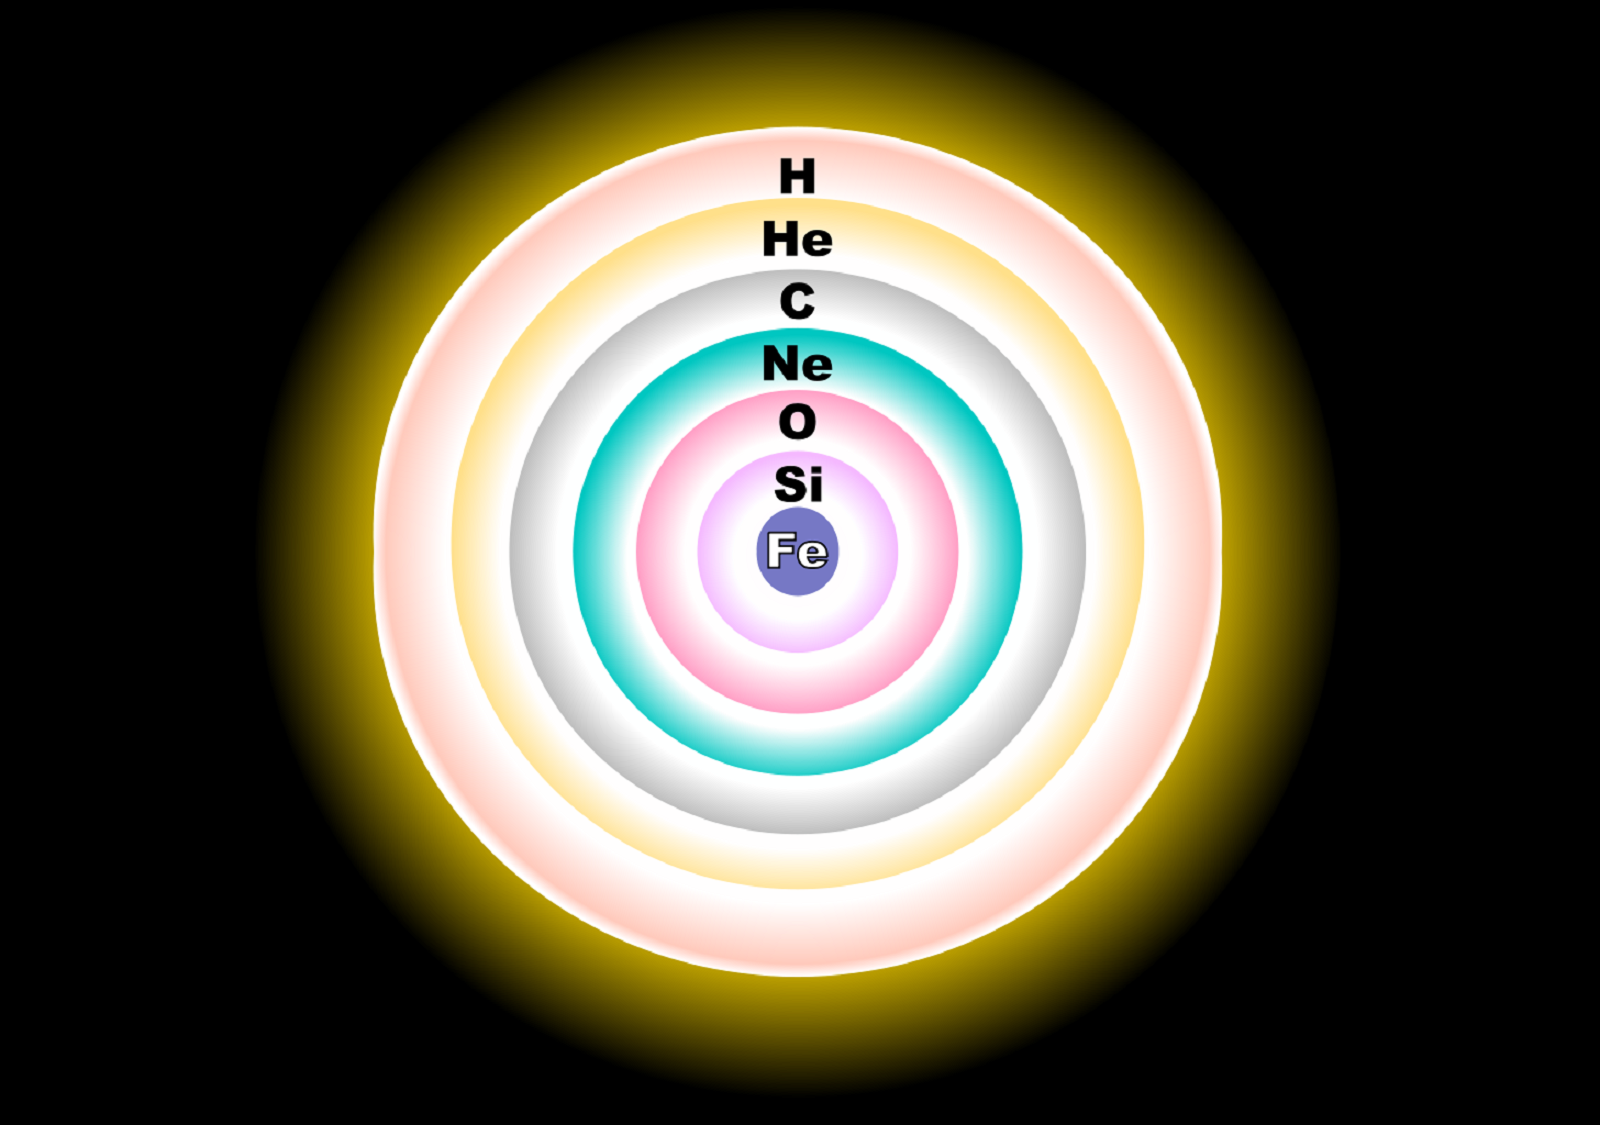
\includegraphics[scale=.25]{images/sncore}
\caption{Esquema no a escala de la estructura de una estrella masiva previo a su explosi\'on como supernova. Los elementos m\'as pesados se alojan en el centro, mientras que  los m\'as livianos, como el hidr\'ogeno o el helio lo hacen en la capa m\'as externa. \textit{Imagen publicada por R. J. Hall en WikiMedia Commons, 15 de agosto de 2007.}}
\label{fig:f0}
\end{figure}


Debido al aumento de temperatura, los electrones del n\'ucleo adquieren energ\'ia cin\'etica suficiente para escapar, desapareciendo as\'i la presi\'on que ejerc\'ian hacia el exterior. Finalmente el n\'ucleo colapsa liberando energ\'ia gravitacional y con ella las capas m\'as externas de la estrella son expulsadas en una gran explosi\'on. Este fen\'omeno se denomina \textit{supernova} e implica un aumento repentino del brillo de una estrella, incrementando su brillo en un factor de $10^8$ veces, pudiendo incluso ser m\'as brillante que la galaxia que la alberga.
\bigskip

En general la variaci\'on de la luminosidad de una supernova corresponde a una curva que crece r\'apidamente los primeros d\'ias (u horas), alcanzando un m\'aximo, para luego decaer. Cabe destacar que existen otros tipos de supernova, c\'omo las de tipo Ia que corresponden a otro fen\'omeno en donde participa una clase de estrella denominada enana blanca junto a otra estrella de cualquier otro tipo. La primera, al poseer una gravedad tan alta en su superficie es capaz de tomar material de su compa\~nera con lo que al superar las 1.44 $M_{\odot}$ se desencadenar\'ia la explosi\'on de una supernova. 
\bigskip

Las supernovas de tipo Ia presentan un decaimiento casi continuo una vez alcanzado el m\'aximo, mientras que las de tipo II presentan dos ca\'idas: una inmediatamente despu\'es de su m\'aximo y otra una vez finalizado un per\'iodo de decaimiento suavizado (ver Figura ~\ref{fig:f1}). Otra forma de diferenciarlas es la presencia de trazas de hidr\'ogeno en los espectros de \'estas: las supernovas de tipo Ia pr\'acticamente no presentan hidr\'ogeno (l\'ineas de absorci\'on distintivas) a diferencia de las de tipo II.\bigskip

\begin{figure}[h!]
\centering
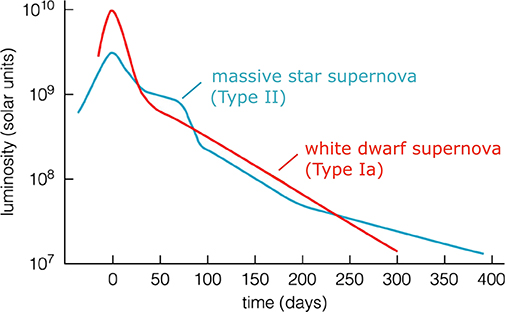
\includegraphics[scale=.8]{images/clear}
\caption{Curvas t\'ipicas de supernovas Ia (enana blanca) y II (estrella masiva). \textit{\textcopyright 2004 Pearson Education Inc., publishing as Addison-Wesley The Bizarre Stellar Graveyard.}}
\label{fig:f1}
\end{figure}


\section{High Cadence Transient Survey: HiTS}

El High Cadence Transient Survey\cite{hits} (desde ahora, HiTS) es un survey cuyo objetivo principal es detectar y seguir fen\'omenos transitorios estelares en escalas de tiempo que van desde horas a d\'ias, con especial atenci\'on a fases tempranas de explosiones de supernovas (primeras horas). Sin embargo, el objetivo original de HiTS corresponde a la detecci\'on de un fen\'omeno llamado \textit{shock breakout} (SBO), un fen\'omeno que ocurre inmediatamente despu\'es del colapso del n\'ucleo de una estrella roja supergigante (una de las posibles etapas finales de una estrella masiva antes de \textit{explotar} en supernova II). Ver Figura \ref{fig:f2}\footnote{$L_{\odot}= 3.828 \times 10^{26}$ W}.

%\ref{fig:f2}\footnote{\url{https://www.nasa.gov/feature/ames/Kepler/caught-for-the-first-time-the-early-flash-of-an-exploding-star}}


\begin{figure}[h!]
\centering
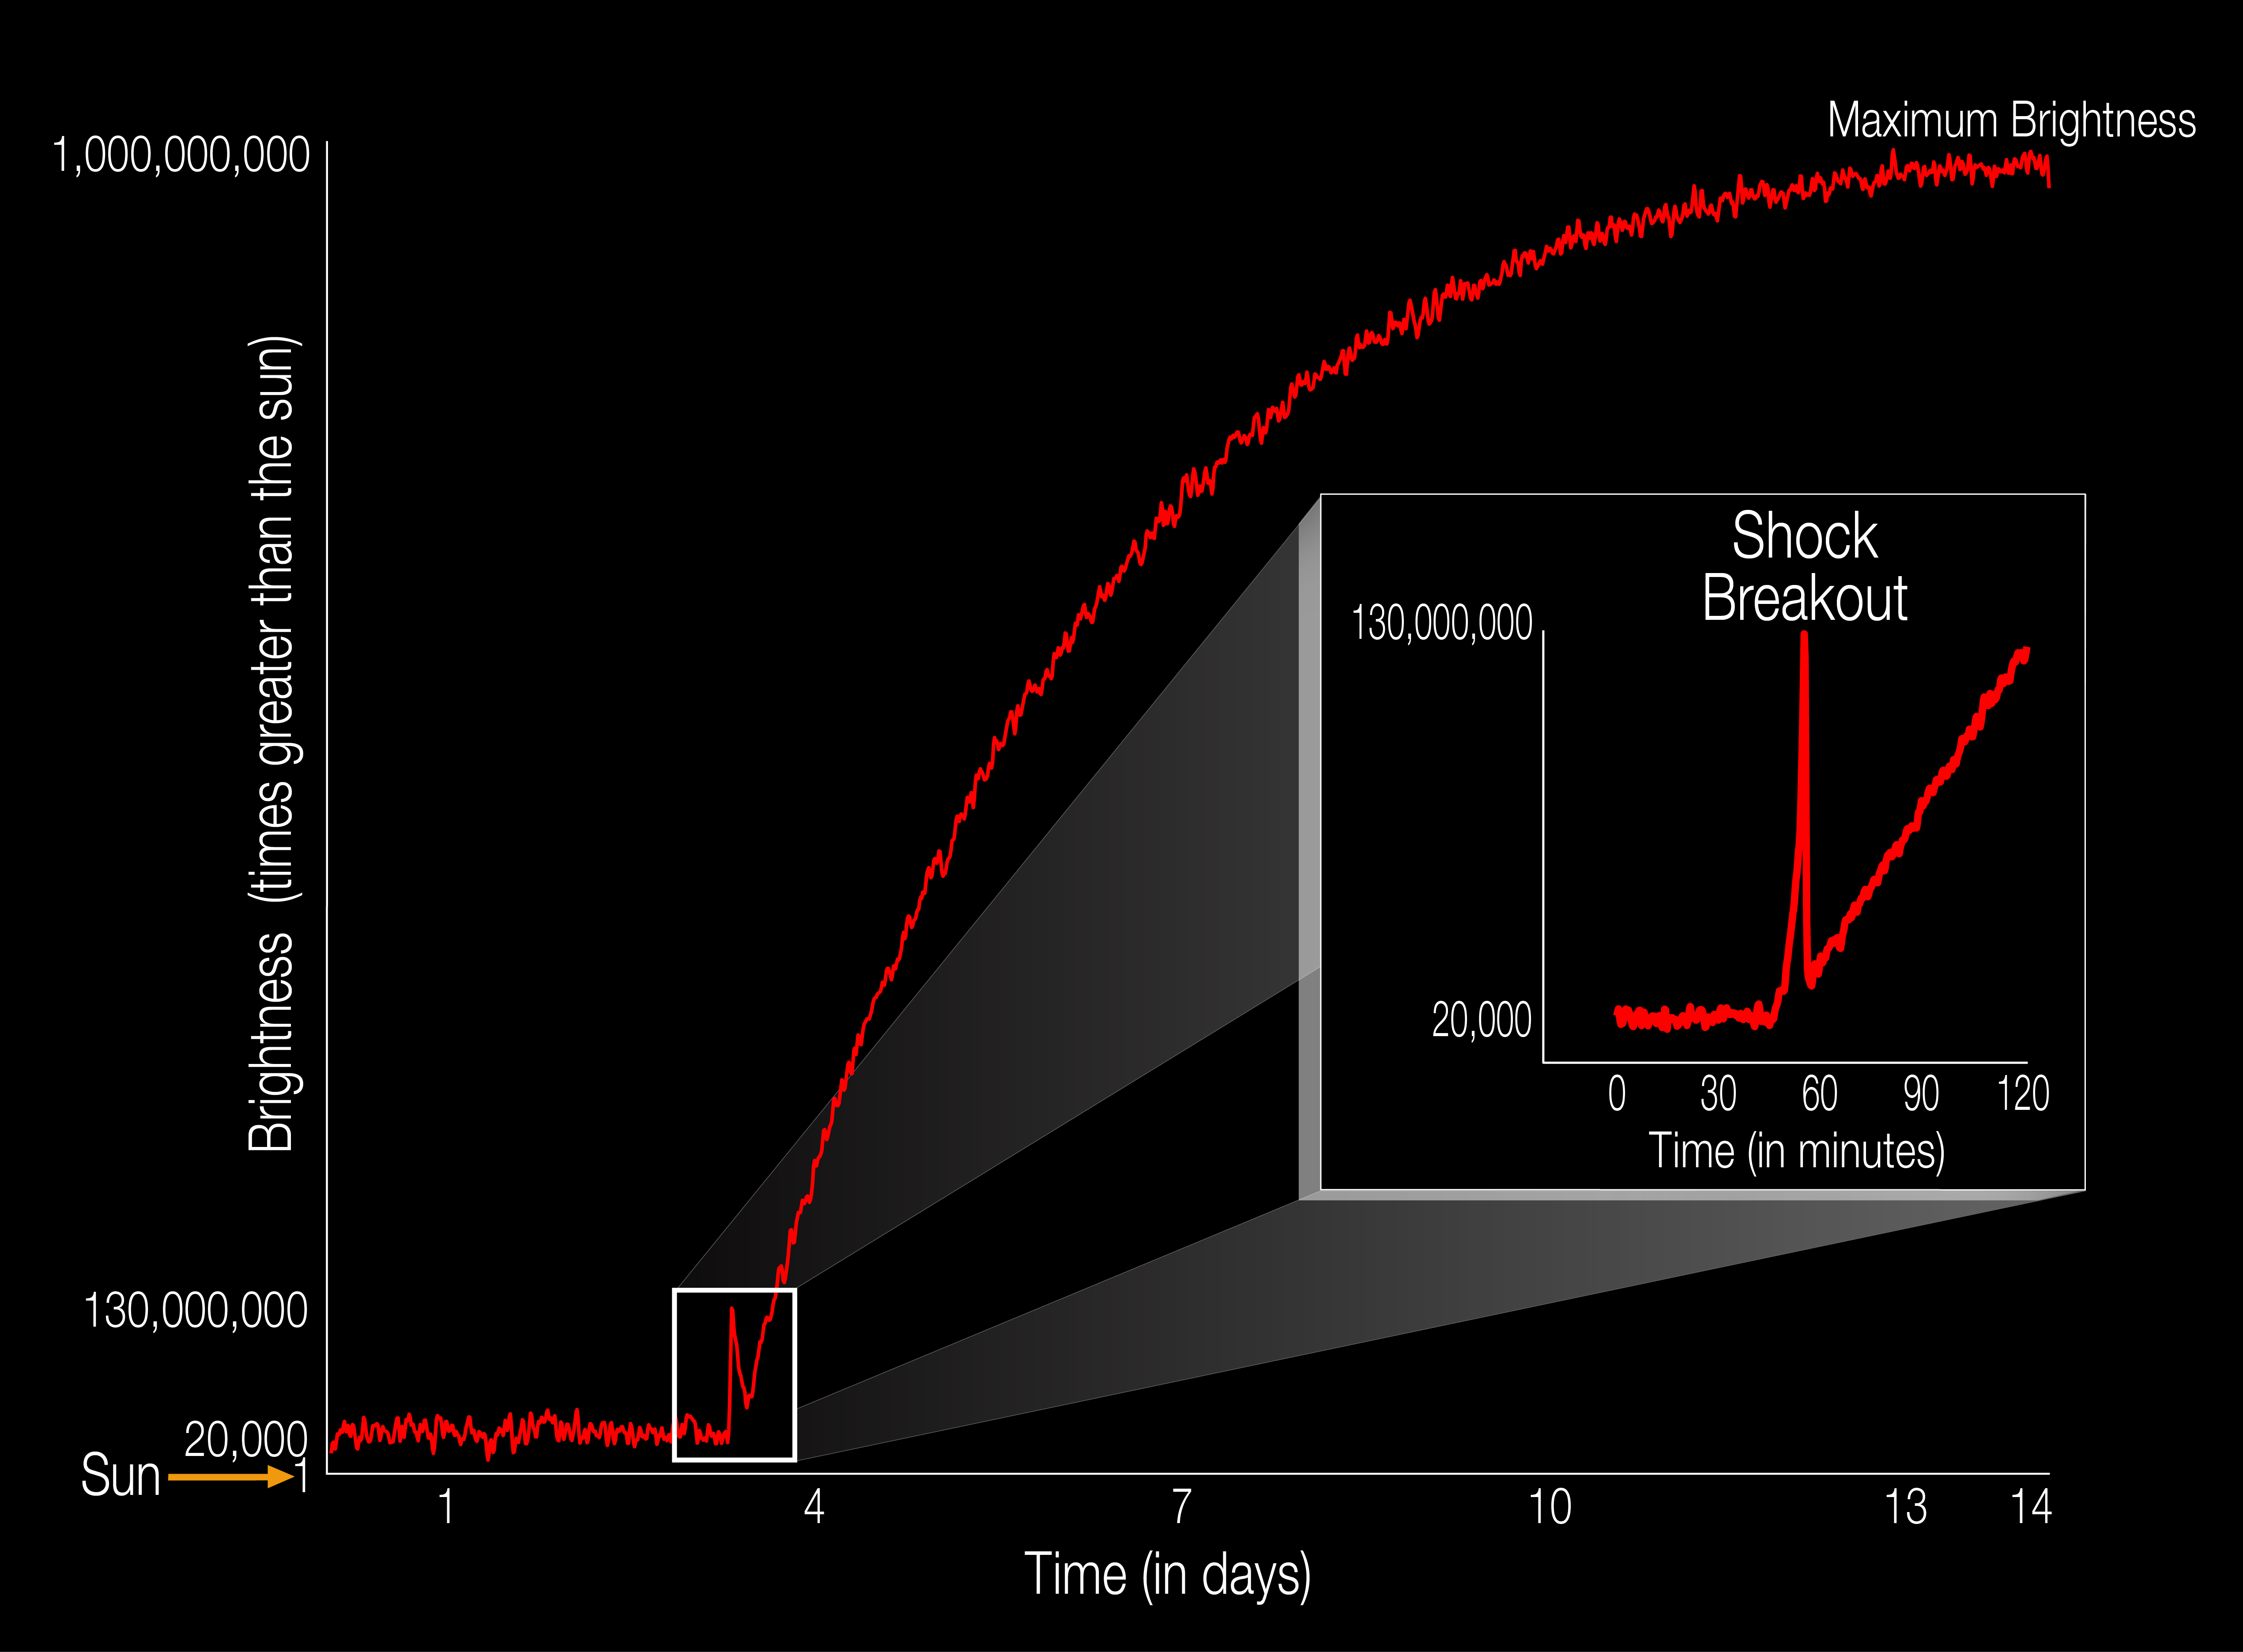
\includegraphics[scale=.25]{images/breakout}
\caption{Diagrama que ilustra la evoluci\'on del brillo de una supernova en t\'erminos de luminosidad solar ($L_{\odot}$) durante d\'ias. Se resalta el fen\'omeno de \textit{shock-breakout} apenas comienza el incremento de la luminosidad de la supernova. Esta imagen fue publicada en la p\'agina de la NASA destacando la primera vez que un evento como este es \textit{capturado} en la banda visible (por el telescopio espacial Kepler). \textit{NASA Ames/W. Stenzel, 2016.}}
\label{fig:f2}
\end{figure}

HiTS utiliza la Dark Energy Camera (DECam, ver Figura \ref{fig:f3}) para la obtenci\'on de sus im\'agenes. Esta c\'amara se encuentra montada en el Telescopio Blanco del Observatorio de Cerro Tololo (CTIO) en la regi\'on de Coquimbo, Chile. Esta c\'amara posee 62 detectores CCD de $2048 \times 4096$ p\'ixeles para la obtenci\'on de im\'agenes cient\'ificas y otros 12 para la gu\'ia, alineamiento y enfoque (ver Figuras \ref{fig:f3} y \ref{fig:f4} d\'onde se muestra disposici\'on de las c\'amaras CCD en el telescopio). 
\bigskip

\begin{figure}[h!]
\centering
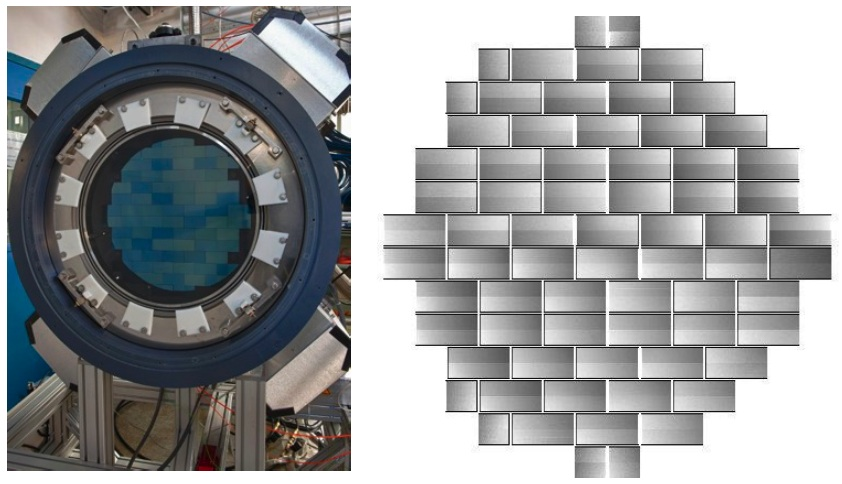
\includegraphics[scale=.5]{images/CCDs.jpg}
\caption{A la izquierda, estructura de la c\'amara DECam poblada con 62 chips CCDs. A la derecha, imagen \textit{flat field} desde DECam. \textit{Im\'agenes tomadas desde la p\'agina del Dark Energy Survey (\url{www.darkenergysurvey.org/the-des-project/instrument/the-camera}).}}
\label{fig:f3}
\end{figure}

Durante el proyecto HiTS se realizaron tres campa\~nas de observaci\'on en los a\~nos 2013, 2014 y 2015 durante el primer semestre de cada a\~no. Se escogieron 40 campos y 4 \'epocas por noche (tambi\'en por campo) para observaciones realizadas en el 2013 y el 2014. Para la campa\~na del a\~no 2015 se escogieron 50 campos. En estas campa\~nas se obtuvieron m\'as de 120 candidatos a supernova. Sin embargo, no se logr\'o encontrar en estas rastros de SBO (Figura \ref{fig:f2}) evento que comprendi\'o uno de los principales objetivos de HiTS. La distribuci\'on de los campos observados, por a\~no, se describe en la Figura \ref{fig:fields}. 

\begin{figure}[h!]
\centering
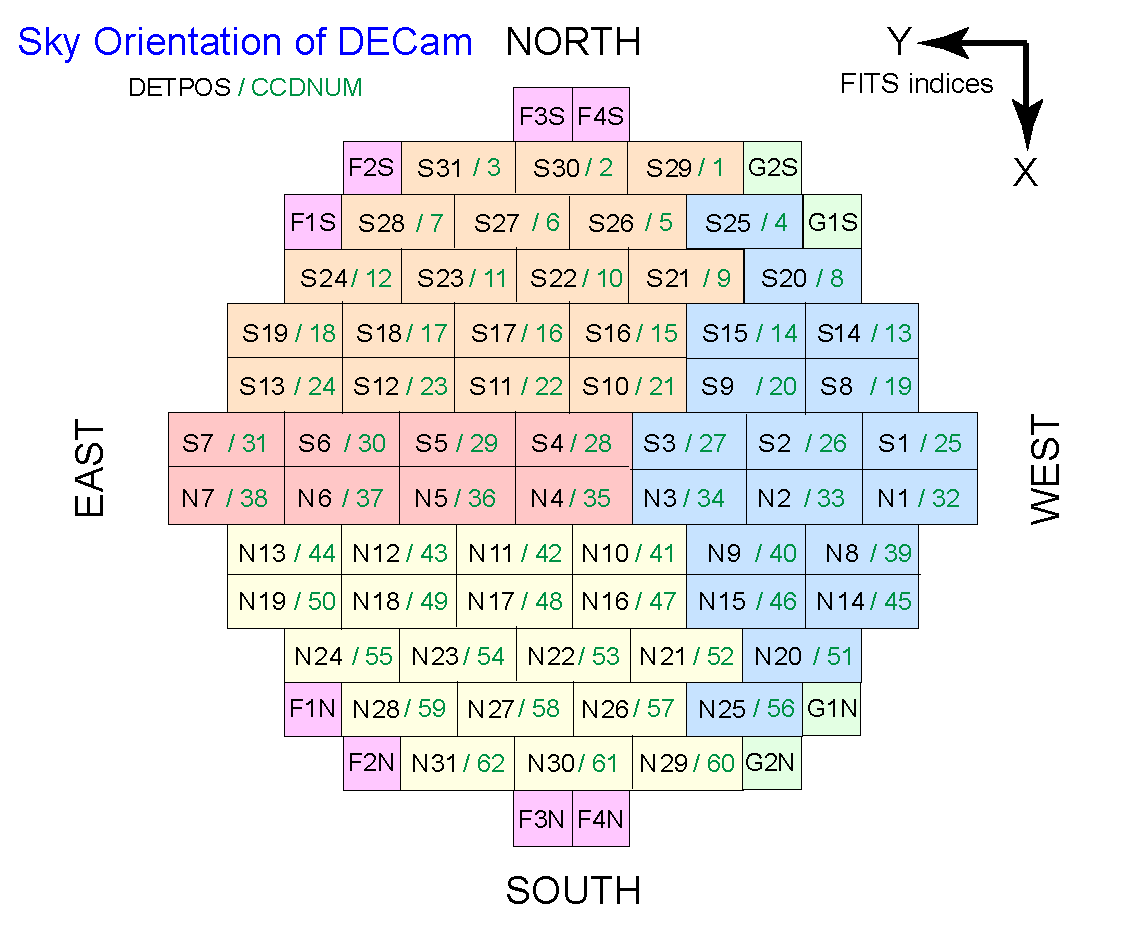
\includegraphics[scale=.75]{images/decam}
\caption{Orientaciones sobre el cielo y la huella espacial del arreglo de detectores en el plano focal. Se destacan los CCD cuya etiqueta comienzan con S o N, ya que estos corresponden a los detectores encargados de obtener las im\'agenes cient\'ificas. El etiquetado de estas componentes puede ser enga\~noso debido a que las iniciales de norte (North) y sur (South) est\'an invertidas en relaci\'on a la orientaci\'on del cielo. \textit{Imagen publicada en el sitio del CTIO (\url{http://www.ctio.noao.edu/noao/node/2250})}.}
\label{fig:f4}
\end{figure}

\begin{figure}
\centering
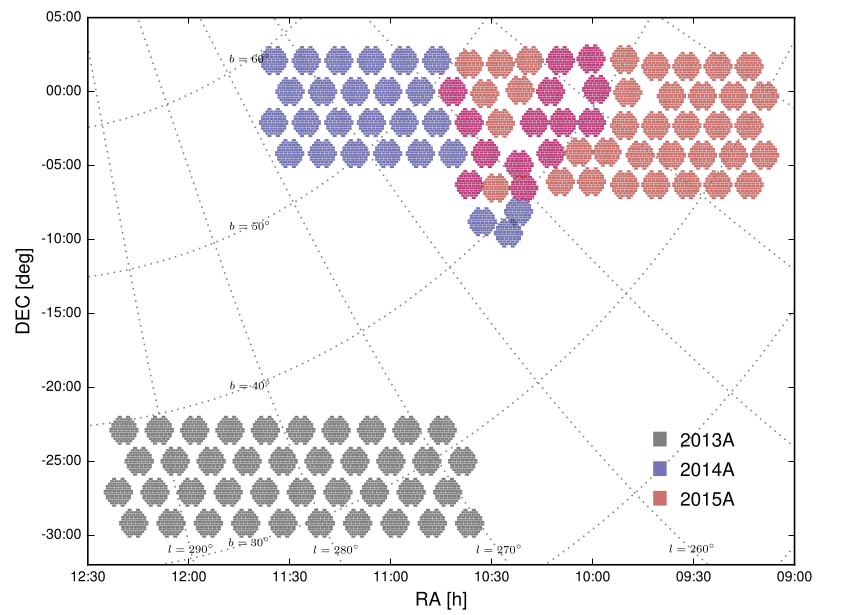
\includegraphics[scale=.5]{images/fields}
\caption{Distribuci\'on espacial de los campos observados durante los primeros semestres de los a\~nos 2013 (gris), 2014 (azul) y 2015 (naranjo). En tono rojo, los mismos campos del a\~no 2015 y 2014 (superposici\'on). \textit{F. F\"orster et al., 2015. HiTS real-time supernova detections.}}
\label{fig:fields}
\end{figure}

\subsection{Datos obtenidos durante el a\~no 2015}\label{ssec:data}
Como se mencion\'o anteriormente, la campa\~na del a\~no 2015 tuvo lugar el primer semestre de ese a\~no. El per\'iodo en que se llev\'o a cabo fue durante los meses de febrero y marzo; espec\'ificamente entre los d\'ias 17 de febrero y 14 de marzo.
\bigskip

El per\'iodo comprendido por los d\'ias 17 a 22 de febrero fue el de mayor latencia, obteni\'endose cinco \'epocas (observaciones) por noche por cada campo. Posteriormente la toma de observaciones cesa y se reanuda a partir del 24 de febrero con una latencia de a lo m\'as tres \'epocas por noche y campo, con interrupciones de hasta nueve d\'ias finalizando el 14 de marzo (ver Figura \ref{fig:cadencia}). 

\begin{figure}
\centering
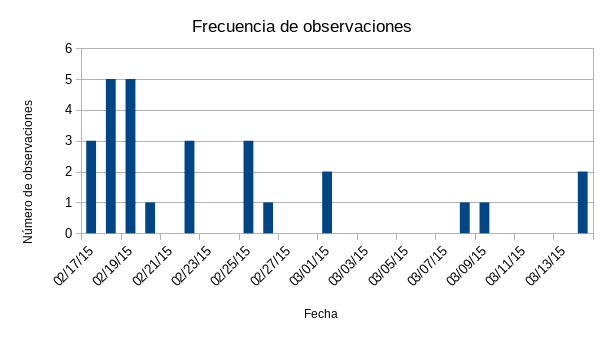
\includegraphics[scale=1.0]{images/cadencia}
\caption{Frecuencia de las observaciones realizadas en el survey de HiTS durante el semestre del a\~no 2015.}
\label{fig:cadencia}
\end{figure}

\section{El filtro de Kalman}
La evoluci\'on determin\'istica de un sistema f\'isico en el tiempo es conocida si el estado del sistema es medido con absoluta precisi\'on en cada instante de tiempo (i.e., en un entorno donde es posible despreciar fen\'omenos cu\'anticos). Sin embargo toda medici\'on est\'a sujeta a incertezas finitas. Para sistemas que son observados en intervalos prolongados de tiempo, se prevee que las diferencias entre los estados estimados y los medidos se incrementen con el tiempo. Para la obtenci\'on de predicciones lo m\'as confiables posible se requiere que el sistema sea regularmente monitoreado y sus estados estimados puedan ser considerados confiables en un lapso de tiempo apropiado. 
\bigskip

Los filtros de Kalman son m\'etodos que proveen un compromiso (o trade-off) entre los valores esperados del estado actual de un sistema y las mediciones que proporcionan informaci\'on de su estado real. La aplicaci\'on de un filtro de Kalman est\'a pensada como un proceso de dos fases:
\begin{enumerate}
\item \textbf{Fase predictiva:} Una \textit{apuesta} del estado actual del sistema que se basa en un modelo f\'isico (determin\'istico). Esta cantidad se denomina usualmente como estado estimado \textit{a priori}. 
\item \textbf{Fase correctiva:} La estimaci\'on del estado \textit{a priori} es corregida con una medida real del sistema con la que se obtiene la predicci\'on; con ella se procede a calcular una cantidad conocida como \textit{ganancia de Kalman} con la que se estima una \textit{aproximaci\'on a posteriori} del sistema, evaluando que tan lejos estuvo nuestra aproximaci\'on \textit{a priori}. 
\end{enumerate}
\bigskip

T\'ipicamente estas fases de predicci\'on y correcci\'on se van alternando mientras se estudia el comportamiento f\'isico de alg\'un sistema. En particular, esto filtros son bastante usados en procesos como el guiamiento de un m\'ovil, en sistemas de navegaci\'on y en an\'alisis de se\~nales; contextos en los cuales el monitoreo de estado de un sistema puede ser m\'as que relevante.
\bigskip

En las subsecciones siguientes se har\'a uso de la notaci\'on de sub\'indices $m|n$, en las estimaciones de estado y covarianzas, para explicitar el instante de tiempo al cual pertenecen:  $m$; y al instante de tiempo de donde se extrae la informaci\'on: $n$. Se har\'a uso de la notaci\'on $k$ para referirse al estado actual y de $k-1$ y $k+1$ para indicar los instantes anterior y pr\'oximo a $k$, respectivamente.
\bigskip

\begin{itemize}
\item $\hat{x}_{k-1|k-1}$: Estado estimado en el paso anterior ($k-1$) o estado inicial del modelo. Es un vector de largo $N$, donde $N$ es el n\'umero de variables de estado a estudiar.
\item $P_{k-1|k-1}$: Matriz de covarianza asociada al estado estimado en el paso anterior o matriz de covarianza inicial. Posee dimensi\'on $N\times N$.
\end{itemize}
\bigskip

Durante la fase predictiva se obtienen las cantidades detalladas a continuaci\'on:
 
\begin{itemize}
\item $\hat{x}_{k|k-1}$: Estado estimado \textit{a priori} (vector de dimensi\'on $N$). 
\item $P_{k|k-1}$: Matriz de covarianza \textit{a priori} (matriz de dimensi\'on $N\times N$ ).
\end{itemize}
\bigskip

Luego, en la fase de correcci\'on se recibe como entrada la medici\'on realizada en el tiempo $k$, $z_k$, y se calculan las siguientes cantidades:

\begin{itemize}
\item $\hat{z}_k$ : Combinaci\'on del estado estimado \textit{a priori}, $\hat{x}_{k|k-1}$ y la medici\'on real, $z_k$. Corresponde a la correcci\'on, propiamente tal.
\item $\tilde{z}_k$ : Diferencia entre la medici\'on real, $z_k$, y la correcci\'on $\hat{z}_k$.
\item $\hat{x}_{k|k}$ : Estado estimado \textit{a posteriori} o estado actualizado.
\item $P_{k|k}$ : Matriz de covarianza \textit{a posteriori} (actializada).
\end{itemize}
\bigskip
 
\begin{figure}
\centering
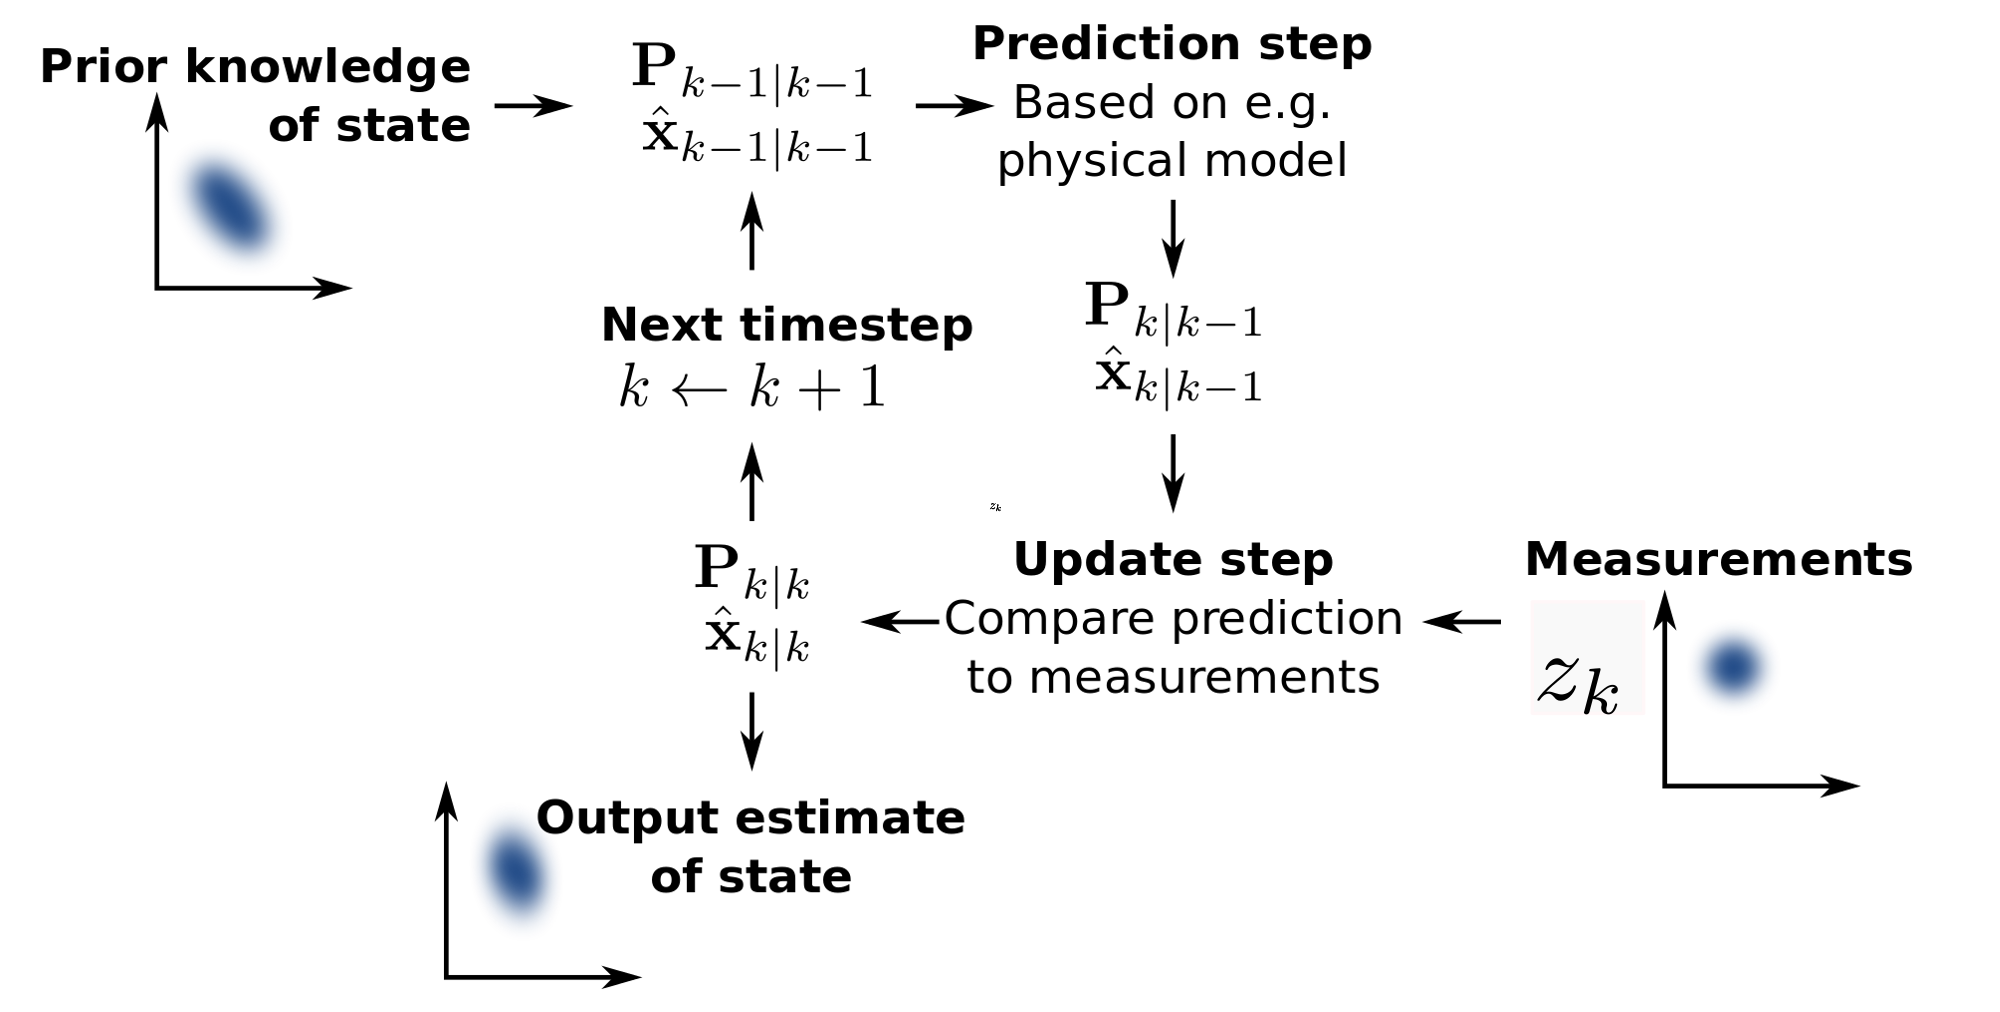
\includegraphics[scale=.2]{images/diag_kalman}
\caption{Diagrama del proceso de estimaci\'on de estados. El filtro de Kalman ``sigue la pista'' del estado f\'isico de un sistema, estim\'andolo paso a paso. El proceso comienza con la entrada de los valores $\hat{x}_{k-1|k-1}$ y $P_{k-1|k-1}$, determinados en el instante $k-1$. Para obtener la estimaci\'on del estado en el instante actual, $k$, se hace una predicci\'on a partir de la informaci\'on m\'as reciente (obtenida en $k-1$) y del modelo f\'isico escogido, obteni\'endose as\'i los valores de $\hat{x}_{k|k-1}$ y $P_{k|k-1}$. Luego durante la fase correcci\'on esta predicci\'on es corregida con la observaci\'on $z_k$ y con ello, se actualizan los valores del estado predicho y de la matriz de covarianza en $\hat{x}_{k|k}$ y $P_{k|k}$, respectivamente. Finalmente estas \'ultimas cantidades se transformar\'an en la entrada del algoritmo para el tiempo $k+1$. \textit{Imagen publicada por P. Aimonen en Wikimedia Commons, en noviembre de 2011.}}
\label{fig:diag}
\end{figure} 
 
El proceso de estimaci\'on (predicci\'on y correcci\'on) puede resumirse en el diagrama de la Figura ~\ref{fig:diag}. 
 
\subsection{Filtro de Kalman B\'asico}
El filtro de Kalman B\'asico \cite{kalman} asume un comportamiento de sistema lineal y que las mediciones y las predicciones siguen una distribuci\'on Gaussiana. 
\bigskip

A continuaci\'on se describen las componentes del desarrollo matem\'atico del filtro:

\begin{itemize}
\item \textbf{$F_k$:} Matriz de transici\'on de estado, de dimensiones $N\times N$.
\item \textbf{$H_k$:} Matriz de transformaci\'on de estado a medici\'on, $K\times N$ (K corresponde al n\'umero de variables de estado medidas en un instante $k$, y puede ser menor a $N$).
\item \textbf{$Q_k$:} Matriz de covarianza del ruido del proceso ($N\times N$).
\item \textbf{$R_k$:} Matriz de covarianza del ruido de las mediciones ($K\times K$).
\item \textbf{$B_k$:} Matriz de control de entrada (contiene alteraciones que se querr\'ian agregar al sistema de manera deliberada, por ejemplo, como la condici\'on de parada de un veh\'iculo en movimiento). Esta matriz es de dimensiones $N\times L$, donde $L$ es la dimensi\'on del vector de control de entrada $u_k$.
\item \textbf{$q_k$:} Corresponde al ruido del proceso modelado, en las variables de estado. Posee una distribuci\'on normal multivariada y centrada en cero, con una matriz de covarianza $Q_k$.
\end{itemize}
\bigskip


Con estas variables, podemos describir las ecuaciones que explican la evoluci\'on del proceso del algoritmo de Kalman b\'asico (un esquema de los c\'alculos involucrados en el proceso de estimaci\'on de estados se puede ver en la Figura \ref{fig:kfb}):
\begin{enumerate}
\item \textbf{Fase predictiva:}\\
Las ecuaciones de estimaci\'on de estado y matriz de covarianza \textit{a priori} son:
\begin{equation}
\hat{x}_{k|k-1} = F_k \hat{x}_{k-1|k-1} + B_k u_k,
\label{eq:eq1}
\end{equation}
\begin{equation}
P_{k|k-1} = F_{k}P_{k-1|k-1}F_k^{T} + Q_k. 
\label{eq:eq2}
\end{equation}
\item \textbf{Fase correctiva:}\\
El proceso de correcci\'on comienza con la determinaci\'on de las siguientes cantidades:
\begin{equation}
\hat{z}_k = H_{k} \hat{x}_{k|k-1},
\label{eq:eq3}
\end{equation}
\begin{equation}
\tilde{z}_k=z_k - \hat{z}_k.
\label{eq:eq4}
\end{equation}

Posteriormente se calcula la matriz de covarianza entre residuos ($S_k$), con la que se calcula la ganancia de Kalman: $K_k$ . Formalmente,
\begin{equation}
S_k = H_k P_{k|k-1} H_{k}^T + R_k,
\label{eq:eq5}
\end{equation}
\begin{equation}
K_k = P_{k|k-1} H_k^T S_k^{-1}.
\label{eq:eq6}
\end{equation}
Con la ganancia de Kalman calculada, se actualiza el valor de la estimaci\'on de estado (\ref{eq:eq7}) y la matriz de covarianza a posteriori (\ref{eq:eq8}), del siguiente modo, 

\begin{equation}
\hat{x}_{k|k} = \hat{x}_{k|k-1} + K_k \tilde{z}_k,
\label{eq:eq7}
\end{equation}

\begin{equation}
P_{k|k} = (I_N - K_kH_k)P_{k|k-1}.
\label{eq:eq8}
\end{equation}
\bigskip

\end{enumerate}

La Figura \ref{fig:kfb} resume el proceso de predicci\'on (obtenci\'on de las cantidades a priori, $\hat{x}_{k|k-1}$ y $P_{k|k-1}$) y correcci\'on (generaci\'on de las estimaciones \textit{a posteriori}  $\hat{x}_{k|k}$ y $P_{k|k}$) del filtro de Kalman B\'asico. 

\begin{figure}[h!]
\centering
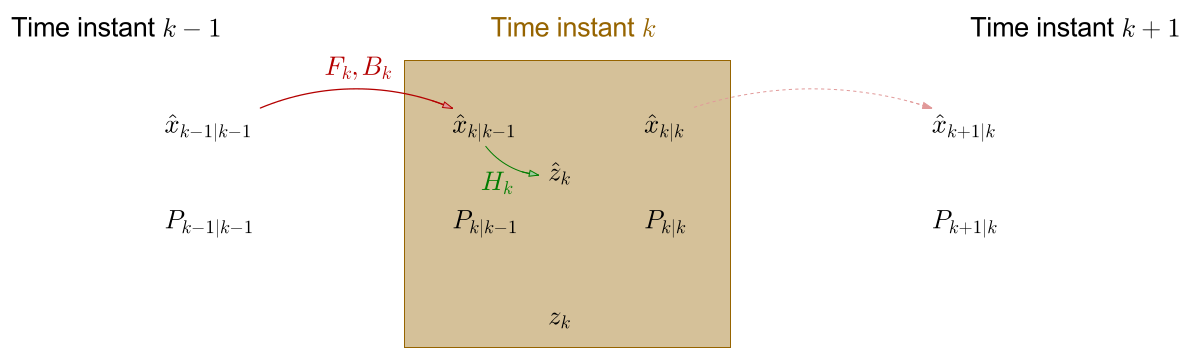
\includegraphics[scale=0.5]{images/kfb}
\caption{Representaci\'on del proceso de predicci\'on (obtenci\'on de cantidades a priori) de las cantidades $\hat{x}_{k|k-1}$ y $P_{k|k-1}$;  y de correcci\'on (estimaci\'on a posteriori) para obtener las cantidades $\hat{x}_{k|k}$ y $P_{k|k}$. Para el siguiente paso, $k+1$, estas estimaciones pasan a ser entrada (\textit{input}) de un nuevo proceso de predicci\'on: $\hat{x}_{k+1|k}$ y $P_{k+1|k}$. \textit{E. Matsinos, 2016. The Kalman Filter: a didactical overview.}}
\label{fig:kfb}
\end{figure}
\subsubsection{Ejemplo: Part\'icula acelerada externamente}
Consideremos un veh\'iculo sobre un riel sin curvas y sin fricci\'on, de tal forma que se pueda asumir un movimiento unidimensional. Inicialmente el veh\'iculo se encontrar\'a en una posici\'on definida como $x_0=0$ y en reposo, $\dot{x}_0=0$, cuando s\'ubitamente es perturbado por fuerzas externas que lo inducen a moverse. Entonces, para monitorear su movimiento se hace un muestreo cada $\Delta t$ segundos. Sin embargo estas mediciones no son del todo precisas, por lo que podr\'ia desearse determinar la posici\'on y velocidad del objeto en cada instante a trav\'es de un modelo.
\bigskip

En esta oportunidad, el vector de estado va a estar dado por:

\begin{align}
x_k &= \begin{bmatrix}
x\\ \dot{x}
\end{bmatrix},
\label{eq:example_state} 
\end{align} 
donde $x$ representa la posici\'on del m\'ovil y $\dot{x}$ su velocidad.
\bigskip

Si asumimos que entre los instantes $k-1$ y $k$, estas fuerzas externas causan una aceleraci\'on constante, $a_k$, cuya distribuci\'on es una normal de media 0 y desviaci\'on est\'andar $\sigma_a$, podemos aplicar las leyes f\'isicas de movimiento, se tiene

\begin{equation}
x_{k} = F_k x_{k-1} + G_k a_k,
\label{eq:example_pred_orig} 
\end{equation}

con 

\begin{align}
F_k &= \begin{bmatrix}
1 & \Delta t\\
0 & 1 
\end{bmatrix},
\label{eq:example_F}
\end{align}


mientras que $G_k$ agrega la componente de aceleraci\'on sobre el sistema:

\begin{align}
G_k &= \begin{bmatrix}
\frac{1}{2} \Delta t^2\\
\Delta t
\end{bmatrix}.
\label{eq:example_G}
\end{align}

De la Ecuaci\'on \ref{eq:example_pred_orig} se desprende que el t\'ermino original $B_k u_k$ ha sido reemplazado por $G_k a_k$; esto se debe a que la \'ultima cantidad corresponde a perturbaciones externas, y no existen entradas de control (perturbaciones controladas o conocidas, por ejemplo, que el riel posea fricci\'on). De esto \'ultimo se deduce que $q_k = G_k a_k$.
\bigskip

De la expresi\'on \ref{eq:example_G} es posible calcular $Q_k$: 

\begin{align}
Q_k = G_k G_k^T \sigma_a^2 &= \begin{bmatrix}
\frac{1}{4}\Delta t^4 & \frac{1}{2}\Delta t^3\\
 \frac{1}{2}\Delta t^3 & \Delta t^2
\end{bmatrix} \sigma_a^2. 
\end{align}

En cada paso temporal $\Delta t$ se realiza una medici\'on, la cual incluye ruido, de la posici\'on del veh\'iculo. Sea $r_k$ el ruido de la medici\'on:

\begin{equation}
z_k = H_k x_k + r_k,
\label{eq:corr_example}
\end{equation}

en donde, $H_k = \begin{bmatrix}
1 & 0
\end{bmatrix}$, y desde la cantidad $r_k$ se calcula $R_k$: $R_k = E[v_kv_k^T]=[\sigma_{z}^2]$.

Con este sistema, podemos modelar el filtro y usar las siguientes condiciones iniciales:

\begin{align}
\hat{x}_{0|0} &= \begin{bmatrix}
0\\
0
\end{bmatrix}
\label{eq:init_state} 
\end{align} 

\begin{align}
P_{0|0} &= \begin{bmatrix}
\sigma_{x}^2 & 0\\
0 & \sigma_{\dot{x}}^2
\end{bmatrix}
\label{eq:init_cov} 
\end{align} 

En donde la Ecuaci\'on \ref{eq:init_state} describe el estado inicial del sistema y \ref{eq:init_cov} la matriz de covarianza inicial, la cual, dependiendo de si se conoce perfectamente la posici\'on del objeto, todos sus valores ser\'an cero; de no conocerse bien la posici\'on del m\'ovil, entonces los valores de $\sigma_{x}$ y $\sigma_{\dot{x}}$ deber\'an considerarse mayores a cero.
\bigskip

Este modelo fue el elegido para estimar la evoluci\'on del flujo y su velocidad en la implementaci\'on de la versi\'on b\'asica del filtro en el programa original (y por consiguiente, en su \textit{refactoring}).
%\begin{equation}
%x_{k|k-1} = F_k x_{k-1|k-1} + G_k a_k
%\label{eq:example_pred} 
%\end{equation}



\subsection{Filtro de Kalman de M\'axima Correntrop\'ia}

El filtro de Kalman basado en m\'axima correntrop\'ia \cite{badong}, difiere del filtro de Kalman tradicional (b\'asico) en que no asume gaussianidad en las observaciones, considerando casos en que una se\~nal puede ser perturbada por pulsos de ruido que sigan una distribuci\'on de cola pesada. En esta oportunidad se utiliza el \textit{criterio de m\'axima correntrop\'ia} del error para el proceso de correcci\'on. 
\bigskip

La correntrop\'ia es una medida de similitud entre dos variables aleatorias. Supongamos, $X,Z \in \mathbb{R}$ con una distribuci\'on conjunta $F_{XZ} (x,z)$. Definimos la correntrop\'ia matem\'aticamente como:

\begin{equation}
V(X,Z) = E[\kappa(X,Z)] = \int \kappa(x,z) dF_{XZ} (x,z),
\label{eq:eqcorr}
\end{equation}
\noindent
donde $E$ representa al operador de esperanza y $\kappa(\cdot,\cdot)$ corresponde a un kernel Mercer invariante a desplazamientos (teorema de Mercer \cite{mercer}). Para este filtro se emplea una funci\'on de kernel Gaussiana, dado por

\begin{equation}
\kappa(x, z) = G_{\sigma} (e) = exp \left(-\dfrac{e^2}{2\sigma^2} \right),
\label{eq:eqkappa}
\end{equation}

donde $e=x-z$ es el error.
\bigskip

Usualmente, en situaciones pr\'acticas, s\'olo se dispone de una cantidad limitada de datos y la distribuci\'on conjunta $F_{XZ}$ podr\'ia ser desconocida, por lo que es posible estimar la correntrop\'ia usando un estimador del promedio sobre la muestra:

\begin{equation}
\hat{V}(X,Z) = \dfrac{1}{M} \sum_{i=1}^N G_{\sigma} (e_i),
\label{eq:eqcoor_est}
\end{equation} 

en que $e_i = x_i - z_i$, con $\{x_i,z_i\}_{i=1}^M$ siendo $M$ el n\'umero de muestras extra\'idas de $F_{XZ}$~\cite{badong}.
\bigskip

Considerando un sistema lineal, descrito por las ecuaciones de estado (\ref{eq:mcc01}) y correci\'on (\ref{eq:mcc02}) 

\begin{equation}
x_{k} = F_{k-1}x_{k-1} + q_{k-1}
\label{eq:mcc01}
\end{equation}
\begin{equation}
\hat{z}_k = H_k x_{k} + r_k.
\label{eq:mcc02}
\end{equation}

Donde $F_{k-1}$ y $H_{k-1}$ corresponden a la matriz de transici\'on de estado y matriz de observaci\'on respectivamente; y los t\'erminos $q_{k-1}$ y $r_k$ corresponden a los vectores de ruido del proceso y de medici\'on, respectivamente, de media cero y matrices de covarianza:
\bigskip

\begin{equation}
\begin{gathered}
E[q_{k-1}q_{k-1}^T] = Q_{k-1}, \\
E[r_{k}r_{k}^T] = R_{k}
\end{gathered}
\end{equation}

Usando la media (donde $\hat{q}_k=0$) y la matriz de covarianza prior, el proceso de predicci\'on queda como: 

\begin{equation}
\begin{gathered}
\hat{x}_{k|k-1} = F_{k-1}\hat{x}_{k-1|k-1},\\
P_{k|k-1} = F_{k-1}P_{k-1|k-1}F_{k-1}^T + Q_{k-1}.
\end{gathered}
\label{eq:mean_pred}
\end{equation}


Luego, la correcci\'on comienza con el c\'alculo de la ganancia de Kalman:

\begin{equation}
K_k = P_{k|k-1} H_k^T (H_kP_{k|k-1}H_k^T + R_k)^{-1},
\label{eq:mcc_kalman_gain}
\end{equation}

y contin\'ua con la determinaci\'on del estado y matriz de covarianza posterior:

\begin{equation}
\hat{x}_{k|k} = \hat{x}_{k|k-1} + K_k(z_k - H_k \hat{x}_{k|k-1}),
\label{eq:mcc_post_state}
\end{equation}

\begin{equation}
P_{k|k} = (I - K_kH_k)P_{k|k-1} (I - K_kH_k)^T + K_kR_kK_k^T
\label{eq:mcc_post_cov}
\end{equation}

donde $I$ corresponde a la matriz identidad (Ecuaci\'on \ref{eq:mcc_post_cov}).
\bigskip

El modelo lineal descrito en las Ecuaciones \ref{eq:mcc01} y \ref{eq:mcc02} pueden reescribirse usando la media prior (\ref{eq:mean_pred}), obteni\'endose:


  \begin{align}
    \begin{bmatrix}
    \hat{x}_{k|k-1}\\
    y_k
	\end{bmatrix}     &= \begin{bmatrix}
          I \\
           H_{k}
         \end{bmatrix} x_k + \nu_k
         \label{eq:nu_det01}
  \end{align} 

\begin{align}
\nu_k &= \begin{bmatrix}
-(x_k - \hat{x}_{k|k-1})\\
r_k
\end{bmatrix} .
\label{eq:nu_det02}
\end{align}

De aqu\'i se desprende, usando las expresiones prior (\ref{eq:mean_pred}), el valor esperado:

\begin{align}
E \lbrack \nu_k \nu_k^T \rbrack &= \begin{bmatrix}
P_{k|k-1} & 0 \\
0 & R_k
\end{bmatrix}\\
&= \begin{bmatrix}
B_{k|k-1; P}B_{k|k-1; P}^T & 0\\
0 &  B_{k|k-1; R}B_{k|k-1; R}^T
\end{bmatrix}\\
& = B_kB_k^T,
\end{align}

donde $B_k$ puede ser obtenido a partir de la descomposici\'on de Cholesky del t\'ermino $E \lbrack \nu_k \nu_k^T \rbrack$ (las cantidades $B_{k|k-1; P}$ y $B_{k|k-1; R}$ corresponden a los valores asociados a la covarianza del estado estimado y del ruido de la medici\'on, $R_k$, respectivamente).
\bigskip

Multiplicando la ecuaci\'on \ref{eq:nu_det01} por la izquierda por $B_k^{-1}$, se obtiene:

\begin{equation}
D_k = W_k x_k + e_k,
\label{eq:D}
\end{equation}

donde $D_k = B^{-1}_k \begin{bmatrix}
\hat{x}_{k|k-1}\\ y_k
\end{bmatrix}$, $W_k = B^{-1}_k \begin{bmatrix}
I\\ H_k
\end{bmatrix}$, $e_k = B^{-1}_k \nu_k$.  
\bigskip

Proponiendo una \textit{funci\'on de costo} basada en la funci\'on de m\'axima correntrop\'ia (ver Ecuaci\'on de correntrop\'ia, \ref{eq:eqcoor_est}):

\begin{equation}
J_{L}(x_k) = \dfrac{1}{L} \sum_{i=1}^L G_{\sigma} (d_{i,k} - w_{i,k}x_k),
\label{eq:costo}
\end{equation}

donde $d_{i, k}$ corresponde al i-\'esimo elemento del vector $D_k$, $w_{i,k}$ es la i-\'esima fila de la matriz $W_k$ y $L$ es la suma de las dimensiones de los vectores de estado ($x_k$), $N$  y medici\'on ($y_k$), $N'$; es decir $L=N+N'$.

Luego, bajo el criterio de m\'axima correntrop\'ia, se tiene que para el estado \'optimo de $x_k$, $\hat{x}_k$

\begin{equation}
\hat{x}_k = \argmax_{x_k} J_{L}(x_k)= \argmax_{x_k} (\sum_{i=1}^L G_{\sigma} (e_{i,k})),
\label{eq:max}
\end{equation}
\bigskip

en que $e_{i,k}$ es el i-\'esimo elemento de $e_k$:

\begin{equation}
e_{i,k}= d_{i, k} - w_{i,k}x_k.
\label{eq:ei}
\end{equation}

Por tanto, la soluci\'on \'optima puede obtenerse resolviendo:

\begin{equation}
\dfrac{\partial J_L(x_k)}{\partial x_k} = \sum_{i=1}^L \lbrack G_{\sigma}(e_{i,k}) w_{i, k}^T (d_{i,k} -w_{i,k}x_k)  \rbrack =0, 
\label{eq:optimal}
\end{equation}
\bigskip

desde donde se tiene:

\begin{equation}
x_k = \lbrace \sum_{i=1}^L \lbrack G_{\sigma} (e_{i,k}) w_{i,k}^T w_{i,k} \rbrack \rbrace^{-1} \times
\lbrace \sum_{i=1}^L \lbrack G_{\sigma} (e_{i,k}) w_{i,k}^T d_{i,k} \rbrack \rbrace
\label{eq:optima1}
\end{equation}

La Ecuaci\'on \ref{eq:optima1} corresponde realmente a una ecuaci\'on de \textit{punto fijo} de $x_k$ (por \ref{eq:ei}) y puede ser reescrita como:

\begin{equation}
x_k = f(x_k) = \left( \sum_{i=1}^{L} \lbrack G_{\sigma} (d_{i,k} - w_{i,k}x_k) w_{i,k}^T w_{i,k}  \rbrack \right)^-1 \times \left( \sum_{i=1}^{L} \lbrack G_{\sigma} (d_{i,k} - w_{i,k}x_k) w_{i,k}^T d_{i,k}  \rbrack \right).
\label{eq:optimal2}
\end{equation}
\bigskip

Un algoritmo iterativo de punto fijo puede ser obtenido usando $\hat{x}_{k, t+1} = f(\hat{x}_{k, t})$, en donde $\hat{x}_{k, t}$ denota la soluci\'on en un punto fijo en la iteraci\'on $t$ (en el instante $k$).
\bigskip

La Ecuaci\'on \ref{eq:optima1} entonces puede ser expresada como:
\begin{equation}
x_k = \left( W^T_k C_k W_k \right)^{-1} W^T_k C_k D_k
\end{equation}

en que $C_k = \begin{bmatrix}
C^{x}_k & 0\\
0 & C^{z}_k
\end{bmatrix} $, con 

\begin{equation}
C^{x}_{k}= diag(G_{\sigma}(e_{1, k}),..., G_{\sigma}(e_{N, k})),
\label{eq:Cx}
\end{equation}

\begin{equation}
{C^{z}_{k}}= diag(G_{\sigma}(e_{N+1, k}),..., G_{\sigma}(e_{N+N', k})).
\label{eq:Cz}
\end{equation}

Con estas derivaciones es posible resumir el algoritmo de estimaci\'on por filtro de Kalman de m\'axima correntrop\'ia como sigue \cite{badong}:

\begin{enumerate}
\item Escoger un $\sigma$ para el ancho del kernel apropiado, y un $\epsilon$ cuyo valor sea $0 < \epsilon < 1$ (lo suficientemente peque\~no para obtener una buena convergencia). Definir un estado estimado inicial $\hat{x}_{0|0}$ y una matriz de covarianza inicial $P_{0|0}$. Definir $k=1$.
\item Usar las Ecuaciones \ref{eq:mean_pred} para obtener $\hat{x}_{k|k-1}$ y $P_{k|k-1}$, y usar descomposici\'on de Cholesky para obtener $B_{k|k-1;P}$.
\item Definir $t=1$ y $\hat{x}_{k|k,0} = \hat{x}_{k|k-1}$, donde $\hat{x}_{k|k,t}$ denota el estado estimado en la iteraci\'on $t$ del algoritmo de punto fijo.
\item Usar los siguientes pasos para calcular $\hat{x}_{k|k}$:

\begin{equation}
\hat{x}_{k|k,t} = \hat{x}_{k|k-1,t} + \tilde{K}_k (z_k - H_k \hat{x}_{k|k-1}),
\end{equation}
con 

\begin{equation}
\tilde{K} = \tilde{P}_{k|k-1} H_k^T (H_k \tilde{P}_{k|k-1} H_k^T + \tilde{R}_k)^{-1}, 
\label{eq:eq14}
\end{equation}

\begin{equation}
\tilde{P}_{k|k-1} = B_{p, k|k-1} \tilde{C}_{x, k}^{-1}B_{p, k|k-1}^T,
\label{eq:eq13}
\end{equation}

\begin{equation}
\tilde{R}_k = B_{r, k} \tilde{C}_{y, k}^{-1}B_{r, k|k-1}^T,
\label{eq:eq12}
\end{equation}

\begin{equation}
\tilde{C^{x}_{k}}= diag(G_{\sigma}(\tilde{e}_{1, k}),..., G_{\sigma}(\tilde{e}_{N, k})),
\label{eq:eq10}
\end{equation}

\begin{equation}
\tilde{C^{z}_{k}}= diag(G_{\sigma}(\tilde{e}_{N+1, k}),..., G_{\sigma}(\tilde{e}_{N+N', k})).
\label{eq:eq11}
\end{equation}


\begin{equation}
\tilde{e}_{i,k} = d_{i,k} - w_{i,k} \hat{x}_{t-1, k|k}.
\label{eq:eq9}
\end{equation}

\item Posteriormente se compara la estimaci\'on de la iteraci\'on actual con la estimaci\'on de la \'ultima:
\begin{equation}
\dfrac{\parallel  \hat{x}_{t, k|k} - \hat{x}_{t-1, k|k} \parallel }{\parallel \hat{x}_{t-1, k|k} \parallel} \leq \epsilon.
\label{eq:eq16}
\end{equation}

Si se cumple la relaci\'on de la Ecuaci\'on \ref{eq:eq16}, entonces $\hat{x}_{k|k} = \hat{x}_{k|k,t}$, y se contin\'ua con el siguiente paso; en caso contrario $t\rightarrow t+1$, y se vuelve al paso (4).

\item Finalmente, se actualiza la matriz de covarianza posterior con 
\begin{equation}
P_{k|k} = \left(I - \tilde{K}_kH_k \right)P_{k|k-1} \left(I - \tilde{K}_k H_k \right)^T + \tilde{K}_kR_k\tilde{K}^T_k,
\label{eq:eq17}
\end{equation}
continuando con el instante $k+1$ en el paso (2).
\end{enumerate}


\subsection{Filtro de Kalman Unscented (UKF)}
\label{ssec:ukf}
Este filtro corresponde a aquel que se pretende agregar a la familia de filtros ya desarrollada en el programa base.
\bigskip

\begin{enumerate}
\item \textbf{Fase predictiva:}\\
En esta versi\'on del filtro \cite{ukf} ya no se habla de matrices de transici\'on de estado, $F_k$, ni de matrices de transformaci\'on de estado-a-medici\'on, $H_k$, sino m\'as bien de funciones diferenciables $f$ y $h$ respectivamente, para describir la transici\'on de estados  y la transformaci\'on de estos a estimaciones a priori. Sin embargo, previo a estas transiciones se deben seleccionar 2N+1 puntos representativos alrededor de $\hat{x}_{k-1|k-1}$ y evaluar estos en la funci\'on no lineal $f$, para obtener las estimaciones de $\hat{x}_{k|k-1}$ y $P_{k|k-1}$. Estos puntos se conocen como \textit{puntos sigma}. En la Figura \ref{fig:fukf} se visualiza el proceso de predicci\'on al momento de obtener el primer conjunto de \textit{puntos sigma}, propagarlos usando la funci\'on $f$ y obtener $\hat{x}_{k|k-1}$ y $P_{k|k-1}$, es decir, la matriz de estados y de covarianza \textit{a priori}. 

\begin{figure}[h!]
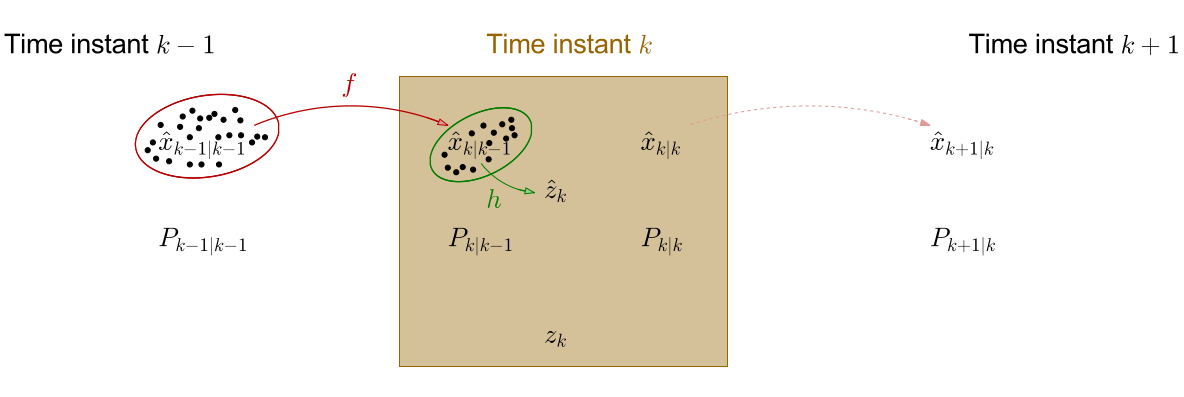
\includegraphics[scale=.5]{images/ukf}
\caption{Representaci\'on del funcionamiento del filtro UKF. En esta oportunidad se hace uso de la funci\'on $f$ y $h$ para obtener las transformaciones $x_{k-1}\rightarrow x_k$ y $x_{k}\rightarrow z_k$. Esto se logra con la evaluaci\'on de los 2N+1 \textit{puntos sigma} generados durante la etapa de predicci\'on (y posteriormente en la etapa de correcci\'on). \textit{E. Matsinos, 2016. The Kalman Filter: a didactical overview.}}
\label{fig:fukf} 
\end{figure}

La generaci\'on de los 2N+1 puntos, se realiza a partir de la \'ultima estimaci\'on $\hat{x}_{k-1|k-1}$  de la siguiente forma:
\begin{equation}
\label{eq:eq18}
\begin{gathered}
\bar{x}_{k-1| k-1}^0 = \hat{x}_{k-1|k-1}\\
\bar{x}_{k-1| k-1}^0 = \hat{x}_{k-1|k-1}+ \chi_i, \quad  \forall i \in [1, N]\\
\bar{x}_{k-1| k-1}^0 = \hat{x}_{k-1|k-1}- \chi_{i-N}, \quad  \forall i \in [N+1, 2N],
\end{gathered}
\end{equation}
donde la cantidad $\chi_i$ corresponde a la i-\'esima columna de la \textit{ra\'iz cuadrada} de la matriz:

 \begin{equation}
 (N+\lambda) P_{k-1 | k-1}.
 \label{eq:eq19}
 \end{equation}
La matriz (\ref{eq:eq19}) puede obtenerse a partir de la descomposic\'on de Cholesky. Por otro lado los puntos sigma se generan junto a dos conjuntos de pesos: $\lbrace w_x^{i} \rbrace$ y $\lbrace w_p^{i} \rbrace$. El primer conjunto se emplea en la estimaci\'on del estado y la predicci\'on del estado, mientras que el segundo conjunto es usado para obtener las matrices de covarianza. Estos pesos son definidos como:
\begin{equation}
\label{eq:eq20}
\begin{gathered}
w^0_x = \dfrac{\lambda}{N+\lambda}\\
w^0_p = w^0_x + 1 - \alpha^2 + \beta\\
w^i_x = w^i_p = \dfrac{1}{2(N+\lambda)}\\
\sum_i^{2N} w^i_x = 1.
\end{gathered}
\end{equation}
De la Ecuaci\'on \ref{eq:eq20} se desprende que los pesos $w_x^i$ son normalizados. Por otro lado, el par\'ametro $\lambda$ se puede escribir en t\'erminos de los valores de $\alpha \in \left( 0,1\right]$ y $\kappa$ seg\'un la expresi\'on siguiente:%\ref{eq:eq21}

\begin{equation}
\label{eq:eq21}
\lambda = \alpha^2  (N + \kappa)- N.
\end{equation}

Los par\'ametros $\alpha$, $\beta$ y $\kappa$ deben ser ajustados acorde al problema que se est\'a estudiando.
\bigskip

Con esto, es posible escribir las ecuaciones de la fase predictiva.
\begin{itemize}
\item Estimaci\'on a priori de los estados. La ecuaci\'on correspondiente es:\\
\begin{equation}
\label{eq:eq22}
\hat{x}_{k|k-1} = \sum_{i=0}^{2N} w_{x}^i f(\bar{x}^i_{k-1|k-1}).
\end{equation}

\item Estimaci\'on a priori de la matriz de covarianza. La ecuaci\'on correspondiente es:\\

\begin{equation}
\label{eq:eq23}
P_{k|k-1} = \sum_{i=0}^{2N} w_p^i \left( f(\bar{x}^i_{k-1|k-1})  - \hat{x}_{k|k-1}\right)\left( f(\bar{x}^i_{k-1|k-1}) - \hat{x}_{k|k-1}  \right)^T + Q_k.
\end{equation}
\end{itemize}


\item \textbf{Fase correctiva:}\\
Durante la fase de correcci\'on, nuevamente se seleccionan 2N+1 puntos representativos, alrededor de $\hat{x}_{k|k-1}$. Estos posteriormente son evaluados en la funci\'on no-lineal $h$.

\begin{equation}
\label{eq:eq24}
\begin{gathered}
\bar{y}_{k-1| k-1}^0 = \hat{x}_{k|k-1}\\
\bar{y}_{k-1| k-1}^i = \hat{x}_{k|k-1}+ \psi_i, \quad  \forall i \in [1, N]\\
\bar{y}_{k-1| k-1}^i = \hat{x}_{k|k-1}- \psi_{i-N}, \quad  \forall i \in [N+1, 2N].\\
\end{gathered}
\end{equation}
La cantidad $\psi_i$ representa la i-\'esima columna de la matriz de \textit{ra\'iz cuadrada} $(N+\lambda)P_{k|k-1}$.

Las ecuaciones del proceso de correcci\'on, por tanto, quedan como sigue:
\begin{itemize}
\item Predicci\'on de las medidas:\\
\begin{equation}
\label{eq:eq25}
\hat{z}_{k} = \sum_{i=0}^{2N} w_x^i h(y_{k|k-1}^{-i}).
\end{equation}
\item Los residuos de las mediciones pueden obtenerse como:\\
\begin{equation}
\tilde{z}_k = z_k - \hat{z}_k.
\label{eq:eq26}
\end{equation}
\item La matriz de innovaci\'on:\\
\begin{equation}
S_k = \sum_{i=0}^{2N} w_p^i (h(y_{k|k-1}^{-i}) - \hat{z}_k)(h(y_{k|k-1}^{-i})^T + R_k.
\label{eq:eq27}
\end{equation}
\item La matriz de covarianza cruzada de estado a medida se describe como:\\
\begin{equation}
C_k = \sum_{i=0}^{2N} w_p^i ( f(\bar{x}^i_{k-1 | k-1})- \hat{x}_{k|k-1} )( h(y_{k|k-1}^{-i}) - \hat{z}_k )^T.
\label{eq:eq28}
\end{equation}
\item La ganancia \'optima finalmente queda:\\
\begin{equation}
K_k = C_kS_k^{-1}.
\label{eq:eq29}
\end{equation}
\item La estimaci\'on \textit{a posteriori} de estado:\\
\begin{equation}
\label{eq:eq30}
 \hat{x}_{k|k} =  \hat{x}_{k|k-1} + K_k \tilde{z}.
\end{equation}
\item Por otro lado, la ecuaci\'on para la matriz de covarianza:\\
\begin{equation}
\label{eq:eq31}
P_{k|k} = P_{k|k-1} - K_kS_kK_k^T.
\end{equation}
\end{itemize}
Los pesos $w_x^i$ y $w_p^i$ son los mismos calculados en la expresi\'on \ref{eq:eq20}, de la fase de predicci\'on.
\end{enumerate}
\bigskip

\subsubsection{Nota}
En este trabajo se considerar\'a un modelo no lineal sobre el paso del tiempo medido desde la primera observaci\'on realizada por el survey: $t_0$. Es decir, la no linealidad no se aplicar\'a sobre la estimaci\'on realizada sobre el paso anterior.

\begin{align}
\begin{bmatrix}
x_k(\Delta t)\\
\dot{x}_k(\Delta t)
\end{bmatrix}  &= \begin{bmatrix}
x_{k-1}\\
0
\end{bmatrix} + \sigma_a\begin{bmatrix}
\Delta t ^{r}\\
\frac{1}{r}\Delta t^{r-1}
\end{bmatrix} = f(x_{k-1}, \Delta t)
\label{eq:modelunscented}
\end{align}

Para la implementaci\'on de este filtro, se usar\'a el modelo descrito en la ecuaci\'on \ref{eq:modelunscented}. El valor de $\sigma_a$ corresponde a un t\'ermino similar al de una aceleraci\'on (como el modelo usado para el filtro b\'asico), para conservar las unidades de posici\'on y velocidad.

\section{Laboratorio Nacional de Computaci\'on de Alto Desempe\~no (NLHPC)}
El National Laboratory for High Performance Computing (NLHPC) es un proyecto asociativo, financiado por el PIA de CONICYT el cual dispone de un potente sistema computacional que est\'a disponible a la comunidad cient\'ifica y acad\'emica nacional (instituciones de investigaci\'on, industria y universidades), estimulando su uso en el desarrollo de \'areas de investigaci\'on que requieran de herramientas computacionales robustas que deban ser usadas de manera intensiva. 
\bigskip

El supercomputador del NLHPC disponible para la comunidad investigadora desde el 2014 en las instalaciones del Centro de Modelamiento Matem\'atico (CMM) de la Universidad de Chile.  

\begin{itemize}
\item 132 nodos de c\'omputo HP (128 nodos HP SL230 y 4 nodos HP SL250), cada uno con dos procesadores de 10 cores Intel Xeon Ivy Bridge E5-2660 V2.
\item 2640 n\'ucleos
\item 6.25 TB de RAM
\item 274TB de almacenamiento Lustre (DDN EXAScaler)
\item 12 co-procesadores Intel Xeon Phi5110p de 2 TFlops
\item Capacidad de c\'omputo de 70 TFlops 
\end{itemize} 

Para la realizaci\'on de este trabajo de t\'itulo se hizo uso de uno de los nodos del cl\'uster de Leftraru, y en la ejecuci\'on de las pruebas se emplearon cuatro cores, 2400 MB por cada CPU (m\'axima RAM permitida) y un \textit{job-array} de largo 93.


%\include{25_linearity}
\chapter{Desempe\~no del programa original}
\label{ch:prev_work}

A continuaci\'on se exponen los resultados de diferentes pruebas realizadas sobre el programa original con la finalidad de medir su desempe\~no computacional en t\'erminos de tiempo de ejecuci\'on y uso de memoria.
\bigskip

Estas pruebas se llevaron a cabo en un computador personal de 8 GB (DDR4) de RAM. La raz\'on de esta  medida (que no se hayan ejecutado en Leftraru) tuvo que ver con que el c\'odigo original contiene demasiadas l\'ineas con el comando \texttt{glob}\footnote{\url{https://docs.python.org/3.5/library/glob.html}} de Python el cual lista reiteradamente el contenido de los directorios de los archivos lo que finalmente termina saturando el nodo destinado para el lanzamiento del programa (en Leftraru el programa no se ejecuta de la misma forma que lo har\'ia localmente, ya que recorre la lista de 93 supernovas de HiTS, repitiendo para cada una de ellas el mismo proceso). Por esto \'ultimo, los administradores del sistema del NLHPC sugirieron modificaciones al programa original, sin embargo, en pos de continuar con el esp\'iritu de esta tesis, se opt\'o por efectuar los experimentos de manera local (usando un computador personal) evitando as\'i introducir m\'as modificaciones (se adapt\'o el programa para Python 3.5, ya que originalmente estaba para 2.7 agregando cambios menores como la forma de imprimir mensajes en consola (\texttt{print})).
\bigskip


Cabe destacar que el problema anteriormente descrito comenz\'o a presentarse una vez que el autor original del mismo pudo corregir la revisi\'on de los nuevos candidatos en el mes de Junio del presente a\~no, debido a que la primera versi\'on del programa s\'olo estaba verificando la presencia de una supernova conocida y no estaba revisando los potenciales nuevos candidatos. Esto se agreg\'o como una continuaci\'on del programa repitiendo pasos como el c\'alculo de flujos, calculo de matrices de estados y sus respectivas predicciones usando alg\'un tipo de filtro de Kalman, etc. El diagrama de la figura \ref{fig:des_sif} entrega una perspectiva general de la secuencia de pasos que realiza el programa.
\bigskip

\begin{figure}[h!]
\centering
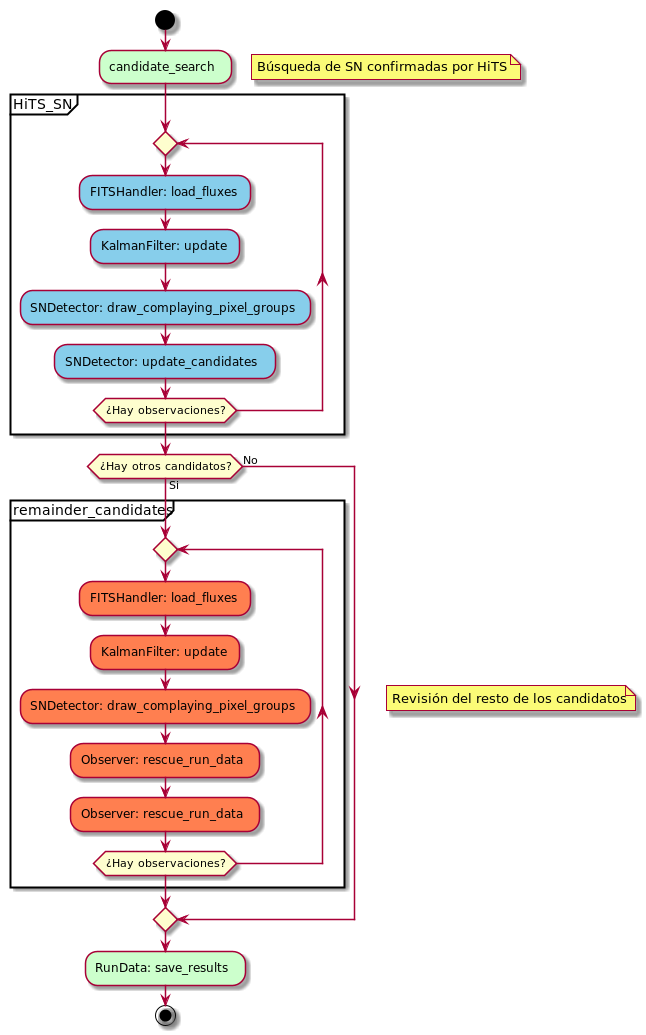
\includegraphics[scale=.5]{images/results/sif_act}
\caption{Diagrama de actividad del programa original. Se aprec\'ian dos ciclos principales: el primero est\'a destinado a la b\'usqueda de una supernova de HiTS, y el segundo a la revisi\'on de la lista de posibles candidatos encontrados durante la verificaci\'on de la supernova de HiTS. Notar que hay pasos que se repiten en la realizaci\'on de ambos an\'alisis.}
\label{fig:des_sif}
\end{figure}

\section{Tiempo de ejecuci\'on}

El estudio del tiempo de ejecuci\'on del programa se realiz\'o usando la funci\'on \texttt{getrusage} de la librer\'ia \texttt{resource} de Python, midiendo el tiempo de usuario en segundos. Las mediciones se realizaron sobre tres conjuntos de datos (las cuales contienen alguna supernova detectada por HiTS) seleccionados al azar: SN14, SN18 y  SN80. En cada uno de ellos comprende secuencias de 26 observaciones. 

\begin{table}[h]
\centering
\begin{tabular}{|l|l|l|l|l|}
\hline
\textbf{ID} & \textbf{C\'alc. Flujos [s]} & \textbf{Aplic. KF [s]} &  \textbf{Agrup. Pixeles [s]}  & \textbf{Actual. Candidatos [s]}\\ \hline \hline
SN14        & 320.98            & 29.39        &  39.98 & 0.01 \\ \hline
SN18            & 290.48             & 23.89         &  36.64  & 0.01\\ \hline
SN80            & 297.79             & 25.40         &   36.88 & 0.01 \\ \hline \hline
Media & 303.08 &  26.23 & 37.83 & 0.01\\\hline 
$\bar{t}/Obs$ & 11.66 &  1.01 & 12.61 & 0.00\\\hline 
\end{tabular}
\label{tab:t1}
\caption{Resultados de tiempos de ejecuci\'on correspondientes a calculo de flujos, estimaci\'on de los filtros, agrupaci\'on de pixeles y filtrado de los mismos durante el peri\'odo de reconocimiento de la supernova correspondiente. Para esta prueba se utiliz\'o el filtro de Kalman B\'asico.}
\end{table}

\begin{table}[h]
\centering
\begin{tabular}{|l|l|l|l|l|}
\hline
\textbf{ID} & \textbf{C\'alc. Flujos [s]} & \textbf{Aplic. KF [s]} &  \textbf{Agrup. Pixeles [s]}  & \textbf{Guardar resultados [s]}\\ \hline \hline
SN14        & 333.59            & 36.13        &  42.22 & 0.09 \\ \hline
SN18            & 289.45             & 24.15         &  36.87  & 0.05\\ \hline
SN80            & 297.90             & 26.39         &   37.59 & 0.06 \\ \hline\hline 
Media & 306.98 &  28.89 & 38.89  & 0.07\\\hline 
$\bar{t}/Obs$ & 11.81 &  1.11 & 1.50 & 0.00\\\hline 
\end{tabular}
\label{tab:t2}
\caption{Resultados de tiempos de ejecuci\'on correspondientes a calculo de flujos, estimaci\'on de los filtros, agrupaci\'on de pixeles y filtrado de los mismos durante el peri\'odo de estudio de los nuevos candidatos encontrados en el paso anterior. Para esta prueba se utiliz\'o el filtro de Kalman B\'asico.}
\end{table}


\begin{table}[h]
\centering
\begin{tabular}{|l|l|l|l|l|}
\hline
\textbf{ID} & \textbf{C\'alc. Flujos [s]} & \textbf{Aplic. KF [s]} &  \textbf{Agrup. Pixeles [s]}  & \textbf{Actual. Candidatos [s]}\\ \hline \hline
SN14        & 327.92            & 731.98        &  38.42 & 0.01 \\ \hline
SN18            & 290.05             & 554.62         &  35.00  & 0.00\\ \hline
SN80            & 309.98             & 628.83         &   37.80 & 0.01 \\ \hline \hline 
Media & 309.32 & 638.48 &  37.07 & 0.01\\\hline
 $\bar{t}/Obs. $& 11.90 & 24.56 & 1.43 & 0.00\\\hline 
\end{tabular}
\label{tab:t3}
\caption{Resultados de tiempos de ejecuci\'on correspondientes a calculo de flujos, estimaci\'on de los filtros, agrupaci\'on de pixeles y filtrado de los mismos durante el peri\'odo de reconocimiento de la supernova correspondiente. Para esta prueba se utiliz\'o el filtro de Kalman de M\'axima Correntrop\'ia.}
\end{table}

\begin{table}[h]
\centering
\begin{tabular}{|l|l|l|l|l|}
\hline
\textbf{ID} & \textbf{C\'alc. Flujos [s]} & \textbf{Aplic. KF [s]} &  \textbf{Agrup. Pixeles [s]}  & \textbf{Guardar resultados [s]}\\ \hline \hline
SN14        & 302.28            & 631.17        &  36.98 & 0.04 \\ \hline
SN18            & 311.63             & 660.51         &  35.68  & 0.06\\ \hline
SN80            & 306.22             & 610.60         &   36.37 & 0.04 \\ \hline \hline
Media & 306.71 & 634.09 &  36.34 & 0.05\\\hline
 $\bar{t}/Obs. $& 11.80 & 24.39 & 1.40 & 0.00\\\hline  
\end{tabular}
\label{tab:t4}
\caption{Resultados de tiempos de ejecuci\'on correspondientes a calculo de flujos, estimaci\'on de los filtros, agrupaci\'on de pixeles y filtrado de los mismos durante el peri\'odo de estudio de los nuevos candidatos encontrados en el paso anterior. Para esta prueba se utiliz\'o el filtro de Kalman de M\'axima Correntrop\'ia.}
\end{table}

\begin{table}[h]
\centering
\begin{tabular}{|l|l|l|l|}
\hline
\textbf{ID} & \textbf{B\'usqueda SN} & \textbf{Revisi\'on candidatos} & \textbf{Tiempo total} \\ \hline
\hline
SN14 & 390.36 & 412.03 & 802.39 \\\hline
SN18 & 351.02 & 350.52 & 701.54\\\hline
SN80 & 360.08 & 361.94 & 722.02 \\\hline\hline
Media & 367.15 & 374.83 & 741.98  \\\hline
 $\bar{t}/Obs. $& 14.12 & 14.42 & 28.54\\\hline 
\end{tabular}
\label{tab:t5}
\caption{Tiempo de ejecuci\'on de los procesos de b\'usqueda de supernova de HiTS, revisi\'on de los candidatos encontrados y tiempo total comprendido por ambos procesos usando filtro de Kalman B\'asico.}
\end{table}


\begin{table}[h]
\centering
\begin{tabular}{|l|l|l|l|}
\hline
\textbf{ID} & \textbf{B\'usqueda SN} & \textbf{Revisi\'on candidatos} & \textbf{Tiempo total} \\ \hline
\hline
SN14 & 1098.33 & 970.47 & 2068.80\\\hline
SN18 & 879.67 & 1007.88 & 1887.55\\\hline
SN80 & 976.62& 953.23& 1929.85\\\hline \hline
Media & 367.15 & 374.83 & 741.98  \\\hline
 $\bar{t}/Obs. $& 14.12 & 14.42 & 28.54\\\hline 
\end{tabular}
\label{tab:t6}
\caption{Tiempo de ejecuci\'on de los procesos de b\'usqueda de supernova de HiTS, revisi\'on de los candidatos encontrados y tiempo total comprendido por ambos procesos usando filtro de Kalman de M\'axima correntrop\'ia.}
\end{table}

\section{Uso de memoria}

La memoria ocupada por el programa se midi\'o en t\'erminos de MiB (Mebibyte) usando la librer\'ia \texttt{memory\_profiler}. Posteriormente las mediciones en la unidad previamente mencionada fueron pasadas a MB\footnote{$1MiB\simeq 1.049$ }

\begin{figure}[h!]
\centering
\subfloat[Memoria ocupada en SN14]{\label{fig:kbf_14}{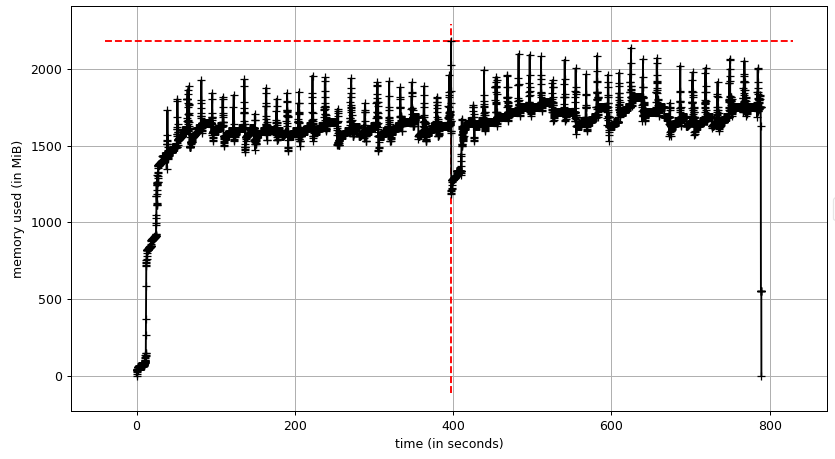
\includegraphics[width=0.5\textwidth]{images/results/sn14_00}}}\hfill
\subfloat[Memoria ocupada en SN18]{\label{fig:kbf_18}{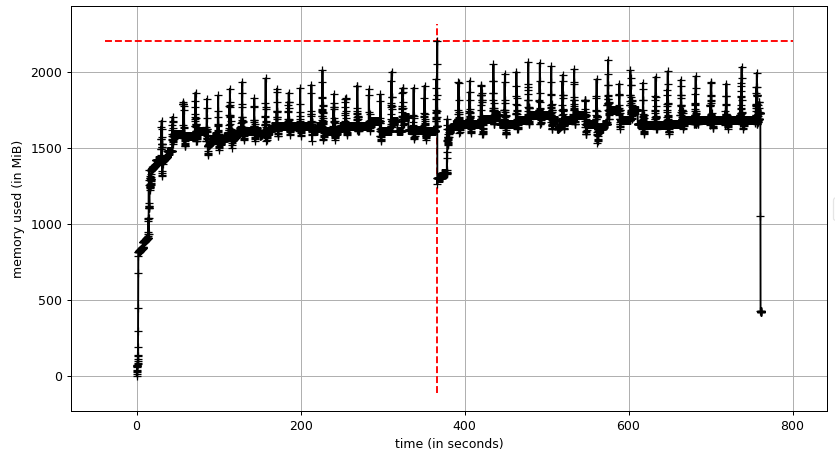
\includegraphics[width=0.5\textwidth]{images/results/sn18_00}}}\vfill
\subfloat[Memoria ocupada en SN80]{\label{fig:kbf_80}{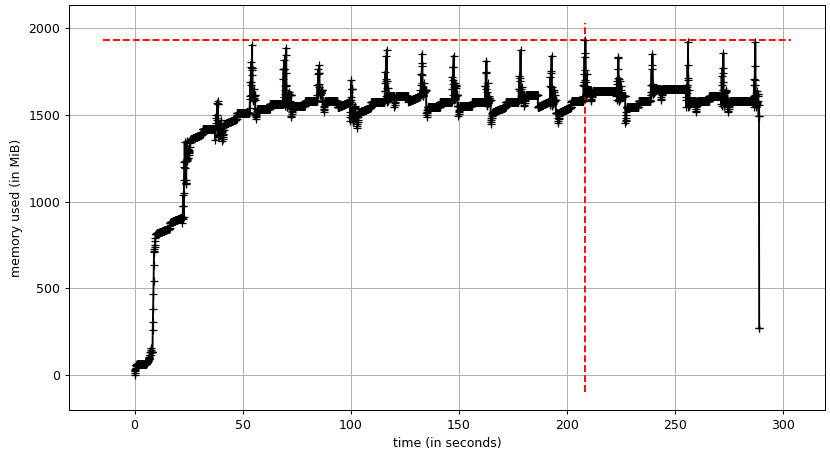
\includegraphics[width=0.5\textwidth]{images/results/sn80_00}}}
\caption{Comportamiento de la memoria (en mebibytes) durante la ejecuci\'on para los tres conjuntos de datos. En los tres lanzamientos se us\'o el filtro de Kalman B\'asico.}
\label{fig:mem_kbf}
\end{figure}

\begin{table}
\centering
\begin{tabular}{|l|l|}
\hline
\textbf{ID} & Memoria [MB]\\\hline\hline
SN14 & 2290.10\\\hline
SN18 & 2314.17\\\hline
SN80 & 2191.82\\\hline
\end{tabular}
\caption{Memoria principal (en unidades de MB) usada durante la ejecuci\'on del programa original usando la versi\'on b\'asica del filtro de Kalman.}
\label{tab:mem1}
\end{table}

\begin{figure}[h!]
\centering
\subfloat[Memoria ocupada en SN14]{\label{fig:mc_14}{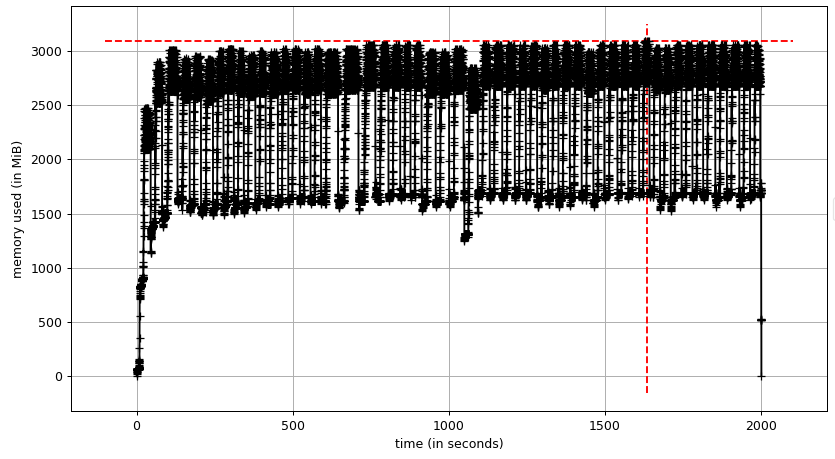
\includegraphics[width=0.5\textwidth]{images/results/sn14_01}}}\hfill
\subfloat[Memoria ocupada en SN18]{\label{fig:mc_18}{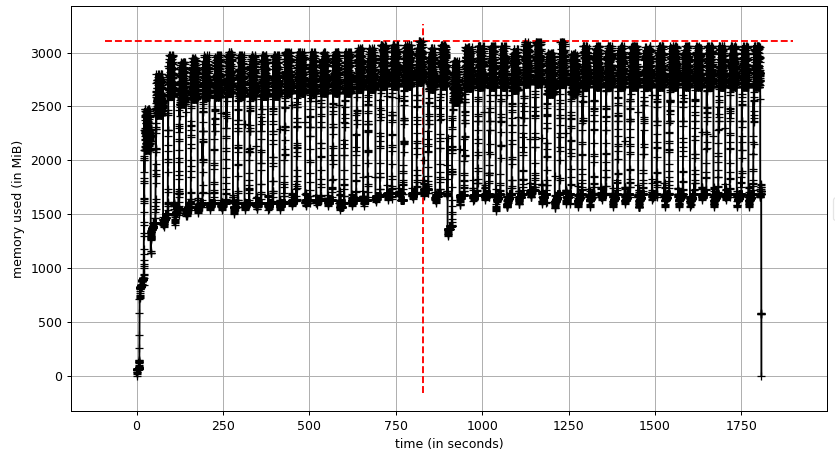
\includegraphics[width=0.5\textwidth]{images/results/sn18_01}}}\vfill
\subfloat[Memoria ocupada en SN80]{\label{fig:mc_80}{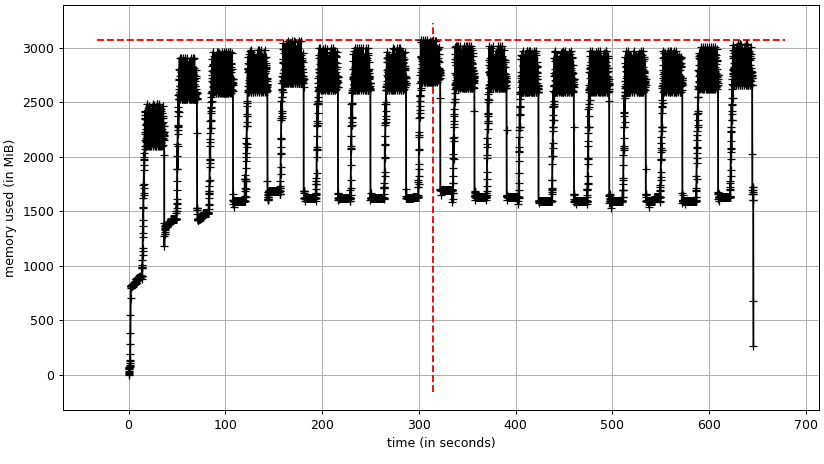
\includegraphics[width=0.5\textwidth]{images/results/sn80_01}}}
\caption{Comportamiento de la memoria (en mebibytes) durante la ejecuci\'on para los tres conjuntos de datos. En los tres lanzamientos se us\'o el filtro de Kalman de correntrop\'ia m\'axima.}
\label{fig:mem_mcc}
\end{figure}

\begin{table}
\centering
\begin{tabular}{|l|l|}
\hline
\textbf{ID} & Memoria [MB]\\\hline\hline
SN14 & 3320.12\\\hline
SN18 & 3248.78\\\hline
SN80 & 3320.12\\\hline
\end{tabular}
\caption{Memoria principal (en unidades de MB) usada durante la ejecuci\'on del programa original usando filtro de Kalman de m\'axima correntrop\'ia.}
\label{tab:mem2}
\end{table}


\chapter{Refactoring}
\label{ch:refactoring}
El refactoring del c\'odigo original se realiz\'o en Python 3.6 (versi\'on diferente a la que el programa fue implementado inicialmente: 2.7). Adem\'as se mantuvieron casi la totalidad de las librer\'ias cambiando \'unicamente Pymorph por Mahotas, debido a que la primera dej\'o de ser mantenida desde el 2010 y corresponde a la librer\'ia para Python 3.   

%\section{Ejecuci\'on de la rutina}
\section{Manejo de datos de entrada}
Toda las im\'agenes de entrada son manipuladas y servidas por la clase \textsc{DataPicker}. Esta clase se inicializa recibiendo un \textit{path} hacia un archivo de configuraci\'on (ver Ap\'endice \ref{subs:a1}) que contiene tanto las rutas a los archivos as\'i como los nombres de estos en t\'erminos de expresiones regulares, semestre a los que corresponde la secuencia de observaciones (los dos \'ultimos d\'igitos del a\~no concatenados con la letra A en caso de corresponder al primer semestre o B al segundo), el campo (representado como un n\'umero de dos d\'igitos, comenzando con cero para valores menores a 10) y el detector CCD (cadena de tres car\'acteres donde el primero de ellos describe a que grupo de detectores corresponde: N o S (ver figura \ref{fig:f4}); adem\'as de un n\'umero entero que va de 1 a 36) como strings. 
\bigskip

El archivo que esta clase consume, para la configuraci\'on de las rutas, debe contener los siguientes campos (ver ejemplo \ref{subs:a1}):
\begin{itemize}
\item \textbf{\texttt{maskDir}}: Directorio donde se almacenan las im\'agenes m\'ascara (im\'agenes que identifican p\'ixeles que no deben ser considerados).
\item \textbf{\texttt{scienceDir}}: Directorio donde se almacenan las im\'agenes cient\'ificas (im\'agenes base ya preprocesadas).
\item \textbf{\texttt{diffDir}}: Directorio donde se almacenan las im\'agenes de diferencia (resta entre las im\'agenes base y su cient\'ifica).
\item \textbf{\texttt{psfDir}}: Directorio donde se encuentran los modelos de psf (ap\'endice \ref{a1:psf}) usados para la determinaci\'on del flujo.
\item \textbf{\texttt{invDir}}: Directorio que guarda las im\'agenes correspondientes a la varianza inversa (\textit{peso} de cada pixel en t\'erminos de ruido: a menor peso, mayor ruido).
\item \textbf{\texttt{afluxDir}}: Directorio que contiene los archivos de extensi\'on \texttt{NPY} dentro de los cuales se guarda el valor de la variable \texttt{aflux}.
\item \textbf{\texttt{maskRegEx}}: Expresi\'on regular con la que es posible identificar el nombre de las im\'agenes m\'ascara en disco siguiendo el path \texttt{maskDir}.
\item \textbf{\texttt{scienceRegEx}}: Expresi\'on regular con la que es posible identificar el nombre de las im\'agenes cient\'ificas en disco siguiendo el path \texttt{scienceDir}.
\item \textbf{\texttt{diffRegEx}}: Expresi\'on regular con la que se identifican el nombre de las im\'agenes de diferencia en disco siguiendo el path \texttt{diffDir}.
\item \textbf{\texttt{invRegEx}}: Expresi\'on regular con la que es posible identificar el nombre de las im\'agenes de la varianza inversa siguiendo el path \texttt{invDir}.
\item \textbf{\texttt{afluxRegEx}}: Expresi\'on regular con la que se identifica el nombre de los archivos \textit{match} que contienen el valor de \texttt{aflux}. Estos archivos est\'an ubicados en el path \texttt{afluxDir}.
\item \textbf{\texttt{psfRegEx}}: Expresi\'on regular que describe el nombre de las im\'agenes que guardan el modelo de PSF en el directorio \texttt{psfDir}.
\end{itemize}


\textsc{DataPicker} maneja  la lectura y preparaci\'on de las im\'agenes a ser analizadas, mientras que un segundo proceso correspondiente a la lectura de resultados anteriores (guardados en un archivo de texto plano) se describir\'a en el Cap\'itulo 5 de nuevas funcionalidades \ref{ch:news}. 
\bigskip
  
\subsection{Lectura y preparaci\'on de im\'agenes}
A continuaci\'on se enumeran los diferentes m\'etodos que intervienen en la recolecci\'on de los datos a ser le\'idos:

\begin{itemize}
\item \textbf{\texttt{config\_reg\_expressions(semester, field, ccd)}}\\
Este m\'etodo recibe como par\'ametros strings que indiquen el semestre (\texttt{semester}), el campo (\texttt{field}) y el ccd (\texttt{ccd}) que se quiere analizar. Puede hacerse uso de los valores de las variables de instancia que la misma clase \textsc{DataPicker} recibe en su constructor. Con estos strings se establecen las rutas de los directorios de las im\'agenes y las expresiones regulares de los nombres de las mismas.
\bigskip

\item \textbf{\texttt{collect\_data()}}\\
Esta funci\'on se encarga de recolectar la ruta completa de las diferentes im\'agenes (m\'ascaras, im\'agenes cient\'ificas, de diferencia, etc.). Para esta finalidad se hace uso del m\'etodo \texttt{walking\_through\_files}. 
\bigskip

\item \textbf{\texttt{walking\_through\_files(regex, dir)}}\\
M\'etodo con el cual se recorren las rutas definidas en los pasos anteriores y se agrupan los nombres completos (directorio incluido) de las im\'agenes ubicadas en el directorio \texttt{dir} y posean un nombre de patr\'on que siga la expresi\'on regular \texttt{regex}.
\bigskip

\item \textbf{\texttt{filter\_science\_images()}}\\
Filtra im\'agenes cient\'ificas de acuerdo a su airmass (Ap\'endice  \ref{ap:airmass}), seleccionando aquellas obtenidas en fechas cuyo valor de airmass calculado es menor a 1,7. De esta secuencia de im\'agenes cient\'ificas resultante se obtiene una lista de fechas que cumplen esta condici\'on medidas en t\'erminos de \textit{d\'ia juliano modificado} o \textit{Modified Julian Date} (MJD) de tipo punto flotante. Estos valores son ordenados de forma creciente.%las fechas en que las observaciones fueron hechas en t\'erminos de \textit{d\'ia juliano modificado} o \textit{Modified Julian Date} (MJD) como variables de punto flotante.
\bigskip

\item \textbf{\texttt{select\_fits(dir)}}\\
Selecciona y ordena los elementos de la lista de im\'agenes de formato fits del directorio \texttt{dir} usando la lista de MJDs (guardada en la variable de instancia \texttt{mjd} de la clase) generada en \texttt{filter\_science\_images()} escogiendo s\'olo aquellas cuyas fechas correspondan a las fechas indicadas.  %cronol\'ogico (i.e. de acuerdo a la secuencia de MJD encontrada en \texttt{filter\_science\_images()}).
\bigskip

\item \textbf{\texttt{select\_npys(dir, ref\_dir, init\_index, n\_pos, rest\_len)}}:\\
Debido a que los archivos de extensi\'on NPY no poseen la variable MJD en su estructura (en los archivos FITS encontramos este valor en el header de la imagen) deben de filtrarse de forma diferente. Para este caso el filtrado de este tipo de archivos se lleva a cabo a trav\'es de la revisi\'on de sus nombres, ya que comparten patrones con los nombres de ciertas im\'agenes fits. Por ejemplo, los nombres de las im\'agenes de PSF, de formato NPY, poseen similitud con los nombres de las im\'agenes FITS de diferencia; igualmente los archivos \texttt{aflux} de formato NPY poseen parecidos en sus nombres con las im\'agenes cient\'ificas. Este parecido es medido a trav\'es de un substring diferente para cada tipo de archivo NPY, definido por la posici\'on inicial \texttt{init\_index}, en el nombre del archivo FITS y largo \texttt{rest\_len}. \texttt{n\_pos} indica la posici\'on de un car\'acter espec\'ifico `` \_ '' en dicho substring para validar esta comparaci\'on.
%Selecciona los archivos de extensi\'on NPY que se encuentran en el directorio \texttt{dir}. Los nombres son filtrados en relaci\'on a las im\'agenes listadas de \texttt{ref\_dir} seg\'un el paso de \texttt{select\_fits(dir)} (es decir, debe ser un directorio que contenga im\'agenes FITS). \texttt{init\_index}, \texttt{n\_pos} y \texttt{rest\_len} son enteros usados para extraer substrings espec\'ificos de los nombres de los archivos.
\end{itemize}

\section{Determinaci\'on de flujos}
El c\'alculo del flujo, en este refactoring, se independiz\'o del manejo de archivos (en el programa orginal estaba alojado en la clase \textsc{FITSHandler}) y se implement\'o en el script \texttt{utils} pensado como librer\'ia.
%El proceso de la obtenci\'on del flujo se simplific\'o, eliminando la clase FitsHandler del programa original. Debido a la posibilidad de hacer los m\'etodos de esta clase est\'aticos se implement\'o un script Python denominada \texttt{utils} para contener estas rutinas e implementarlas est\'aticamente.
\bigskip

Los m\'etodos que participan en la rutina de calculo de flujo son: 

\begin{itemize}
\item \textbf{\texttt{naylor\_photometry(invvar, diff, psf)}\cite{naylor}:}\\
Calcula el producto del flujo por su varianza. Retorna el producto y la varianza. Para esto obtiene el flujo a partir de la imagen PSF entregada (\texttt{psf}) y del producto entre la imagen diferencia y la de varianza inverza (\texttt{diff} y \texttt{invvar} respectivamente).
\bigskip


\item \textbf{\texttt{calc\_fluxes(diff, psf, invvar, aflux)}:}\\
Calcula el flujo y su varianza gestionando la entrada y la salida de \texttt{naylor\_photometry(invvar, diff, psf)}. Los valores NaN son transformados a valores de punto flotante de constante 0.001.
\end{itemize} 

Estos m\'etodos  son llamados desde la rutina \textsc{RoutineHandler} (ver Cap\'itulo \ref{ch:news}).
\section{Filtros originales}
La refactorizaci\'on de los filtros de Kalman originales implic\'o la implementaci\'on de nuevas clases e interfaces para el desarrollo del patr\'on propuesto: Strategy (ver familia de m\'etodos resultante en la figura \ref{fig:ref1}). A continuaci\'on se presentan cada una de ellas:

\begin{itemize}
\item \textbf{IPredict:} Interface que describe el comportamiento de la funci\'on \textsc{Predict} de un filtro de Kalman. \texttt{predict} recibe como par\'ametros el paso de tiempo ($\Delta t$), la matriz de estado, la matriz de covarianza de estado, y las predicciones de las matrices de estado y covarianza determinadas en el paso anterior (con la finalidad de actualizar estas variables). Su firma queda como:
\begin{center}
\texttt{predict(delta\_t, state, state\_cov, pred\_state, pred\_cov)}
\end{center}
Este m\'etodo entrega finalmente las matrices de estado y covarianza de estado predicho.
\bigskip

\item \textbf{ICorrect:} Interface que describe el comportamiento de la funci\'on \textsc{Correct} de un filtro de Kalman. \texttt{correct} recibe como par\'ametros el matriz de flujo (\texttt{z}) y de varianza de las observaciones (\texttt{R}), la matriz de estado predicha, la matriz de covarianza predicha, la matriz de estado y la matriz de covarianza (para sobreescritura) obtenidas en el paso anterior. Su firma queda como:
\begin{center}
\texttt{correct(z, R, pred\_state, pred\_cov, state, state\_cov)}
\end{center}
\bigskip
Esta funci\'on entrega finalmente las matrices de estado y covarianza de estado corregido.

\end{itemize}

\subsection{Predicci\'on}
\textbf{LinearPredict:} Clase que extiende de IPredict. Implementa m\'etodo \texttt{predict} que ser\'a usado tanto por el filtro b\'asico como el de m\'axima correntrop\'ia. Su instanciaci\'on recibe como argumento \texttt{sigma\_a} (desviaci\'on est\'andar del modelo, asumiendo una distribui\'on gaussiana en la distribuci\'on de las observaciones).
\bigskip


\subsection{Correcci\'on}
\textbf{BasicCorrect:} Clase que extiende de ICorrect. Implementa m\'etodo \texttt{correct} que ser\'a usado para el tipo de filtro de Kalman B\'asico.
\bigskip

\textbf{MCCorrect:} Clase que extiende de ICorrect. Implementa m\'etodo \texttt{correct} que ser\'a usado para el tipo de filtro de Kalman de m\'axima correntrop\'ia. El constructor de esta clase recibe los siguientes par\'ametros:

\begin{itemize}
\item \texttt{epsilon}: Cantidad con la cual se contrastar\'a el error o precisi\'on que se quiera lograr con la estimaci\'on.
\item \texttt{max\_iter}: N\'umero m\'aximo de iteraciones.
\item \texttt{silverman}: \textit{boolean}. Determina si se usa o no la apoximaci\'on de Silverman para el ancho de banda del kernel Gaussiano.
\item \texttt{std\_factor}: Factor de desviaci\'on est\'andar usado en la aproximaci\'on de Silverman.
\item \texttt{sigma}: Sigma usado para el kernel Mercer.
\end{itemize}

\subsection{Filtros refactorizados}

\begin{itemize}
\item \textbf{KalmanFilter:} Clase abstracta padre de los subtipos BasicKalmanFilter y MCKalmanFilter. Posee los m\'etodos abstractos \texttt{predict} y \texttt{correct}, que son definidos de acuerdo a las estrategias de predicci\'on y correci\'on descritas previamente.
\item \textbf{BasicKalmanFilter:} Representa el filtro b\'asico de Kalman. Est\'a compuesto por las estrategias \texttt{LinearPredict} y \texttt{BasicCorrect}.
\item \textbf{MCKalmanFilter:} Representa el filtro de m\'axima correntrop\'ia. Est\'a compuesto por las estrategias \texttt{LinearPredict} y \texttt{MCCorrect}.
\end{itemize}
\bigskip

\begin{figure}
\centering
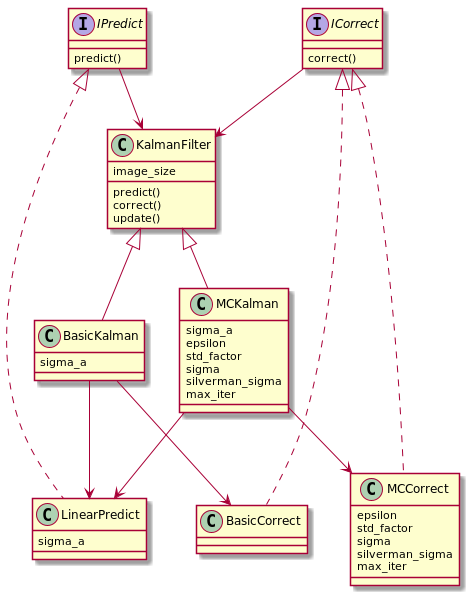
\includegraphics[scale=.5]{images/kalmanfilter_class}
\caption{Familia de filtros de Kalman y patr\'on \textit{strategy} usado en la implementaci\'on de los m\'etodos \texttt{predict} y \texttt{correct}.}
\label{fig:ref1}
\end{figure}

\section{Detecci\'on de candidatos}
Mientras que la detecci\'on de candidatos en el programa original se realiza en una instancia de la clase \textsc{SNDetector}, la detecci\'on en la nueva versi\'on se realiza en SourceFinder, el cual funciona de la misma forma que su antecesor. El cambio de nombre representa la intencionalidad de extender la funcionalidad de esta clase no s\'olo a la detecci\'on de supernovas sino adem\'as encontrar objetos como estrellas variables.
\bigskip

Su constructor requiere los siguientes argumentos:
\begin{itemize}
\item \texttt{flux\_thresh:} Umbral de corte para el flujo estimado por el filtro de Kalman.
\item \texttt{flux\_rate\_thresh:} Umbral de corte de velocidad de flujo estimado por el filtro de Kalman.
\item \texttt{rate\_satu:} Tasa de saturaci\'on en la velocidad de flujo.
\item \texttt{accum\_neg\_flux\_depth:} Cantidad de \'epocas de registro de p\'ixeles negativos (para la construcci\'on de una matriz de booleans de esta profundidad).
\item \texttt{accum\_med\_flux\_depth:}: Cantidad de \'epocas de registro de p\'ixeles cuya intensidad mediana (durante las \'epocas) es mayor a 1500.
\item \texttt{image\_size:} Dimensi\'on de las im\'agenes FITS.
\item \texttt{n\_consecutive\_obs:} N\'umero de alertas u observaciones consecutivas a considerar para confirmar una detecci\'on.

\end{itemize}
%La detecci\'on de candidatos en el programa original se realiza en \textsc{SNDetector}, sin embargo, durante este refactoring se descompuso el proceso de reconocimiento de fuentes estelares (grupo de pixeles brillantes) del proceso de selecci\'on de candidatos, siendo este \'ultimo la continuaci\'on del primero. Por tanto se crearon las clases \textsc{SourceFinder} para el filtrado y agrupamiento de pixeles y \textsc{TPDetector} (transient phenomena detector) para la revisi\'on de las \textit{fuentes} encontradas en el paso anterior.
\subsection{SourceFinder}
La clase \textsc{SourceFinder} posee los siguientes m\'etodos:
\begin{itemize}
\item \texttt{pixel\_discard}:\\
M\'etodo en el que se realiza el descarte de p\'ixeles de forma individual, siguiendo los siguientes criterios:
\begin{enumerate}
\item Si el flujo estimado por el filtro de Kalman para un pixel es menor que el umbral dado.
\item Si la velocidad de flujo estimada por el filtro de Kalman es menor que el umbral  de la velocidad de flujo multiplicado por un factor determinado la tasa de saturaci\'on en la velocidad de flujo y el flujo estimado por el filtro.
\item Si un pixel de la imagen cient\'ifica es menor a la mediana m\'as cierto delta (en este trabajo, siguiendo la l\'inea de desarrollo de P. Huentelemu \cite{huentelemu}, se consider\'o 5.0) es descartado.
\item Si las varianzas de flujo son mayores a 150.0 (valor estimado por el autor del software original \cite{huentelemu}).
\item Si las varianzas de la tasa de cambio de flujo (o velocidad de flujo) es mayor o igual a 150.0.
\item Si los p\'ixeles no caen en etiquetas de invalidaci\'on dentro de la m\'ascara que ha sido procesada para marcar tambi\'en los p\'ixeles vecinos a los realmente defectuosos.
\item Si los p\'ixeles no han ca\'ido dentro del descarte por superar la mediana estimada a partir de cuatro \'epocas. 
\end{enumerate}
\item \texttt{grouping\_pixels()}:\\
Este m\'etodo trabaja con las etiquetas determinadas en el paso anterior en un arreglo de matrices (\texttt{numpy array}) denominado \texttt{pixel\_flags} (variable de instancia). Adem\'as recibe el \'indice de MJD correspondiente a la observaci\'on de tal fecha.
La agrupaci\'on de p\'ixeles se realiza gracias a funciones brindadas por la librer\'ia \textsf{Mahotas}, usando el m\'etodo \texttt{label} para encontrar dominios cerrados en el mapa de p\'ixeles validados.
\bigskip

\item \texttt{filter\_groups(science, flux, var\_flux, state, base\_mask)}:\\
Este m\'etodo recibe la imagen cient\'ifica, el flujo y su varianza, el estado determinado por el filtro de Kalman y la m\'ascara correspondiente a una \'epoca espec\'ifica. 
El filtrado de grupos de p\'ixeles se lleva a cabo bajo las siguientes reglas de descarte: 

\begin{enumerate}
\item Descarte de grupo por contener posible mala resta alrededor (valores negativos).  
\item	Si no hay m\'aximos locales dentro del grupo de p\'ixeles encontrados dentro de la imagen cient\'ifica.
\item	Si no hay m\'aximos locales dentro del grupo de p\'ixeles encontrados dentro de la matriz de flujo (calculado por \texttt{calc\_fluxes}).
\item	Si no hay m\'aximos locales dentro del grupo de p\'ixeles encontrados dentro de la matriz velocidad de flujo.
\item 	Si los valores de los p\'ixeles superan la mediana local en imagen cient\'ifica.
\item	Si el grupo posee alg\'un pixel que doble el valor del flujo o de la imagen cient\'ifica.
\item	Si el centro del grupo se encuentra etiquetado como defectuoso dentro de la m\'ascara.
\item	Si el pixel del centro del grupo se encuentra rechazado al ser superior a la mediana de los p\'ixeles de cuatro observaciones consecutivas.
\item	Si la varianza del flujo del pixel del centro del grupo es mayor al determinado por el umbral.
\end{enumerate} 
\item \texttt{update\_candidates(mjd):}\\
En la estructura \texttt{CandData} se van registrando fechas (MJD) en que se han detectado candidatos previamente o se han detectado por primera vez. Es una estrutura tipo lista en la que se van guardando diccionarios que contienen, cada uno, las coordenadas de un objeto, las \'epocas en las que ha sido detectado y si corresponde o no a una supernova conocida.

\item \texttt{check\_candidates(SN\_index, SN\_pos):}\\
Verifica que dado un \'indice de supernova (\texttt{SN\_index}) y sus coordenadas \texttt{SN\_pos} se ha detectado dentro de los candidatos encontrados. 

\item \texttt{draw\_complying\_pixel\_groups(science, state, state\_cov, base\_mask, dil\_mask, flux, var\_flux, mjd)}:\\
Este m\'etodo es el que llama a \texttt{pixel\_discard} para etiquetar p\'ixeles para el descarte y no ser considerados en el paso de agrupamiento al llamar a \texttt{grouping\_pixels}. Luego se invoca el m\'etodo \texttt{filter\_groups} para hacer el descarte a nivel grupal y obtener candidatos. La \'ultima llamada es para el m\'etodo \texttt{update\_candidates} para actualizar lista de candidatos encontrados en la variable de instancia \texttt{CandData}.
\bigskip

Como argumentos recibe todos los elementos necesarios para ejecutar los m\'etodos que llama.
%\texttt{save\_data} que se encuentra en clase \textsc{DataContent}. 

\end{itemize}

\section{Visualizaci\'on de resultados}
En el proceso de visualizaci\'on participan dos clases: \textsc{Observer} y \textsc{Visualizer}. La primera clase es la encargada de generar una lista de diccionarios dentro de los cuales se almacena informaci\'on de los candidatos encontrados durante el proceso de detecci\'on. Esta lista es guardada como una variable de instancia en \textsc{Observer} denominada \texttt{objects} y la informaci\'on contenida por cada uno de los diccionarios corresponde a las siguientes componentes:

\begin{itemize}
\item Ubicaci\'on del objeto en la primera imagen cient\'ifica procesada, como un arreglo de \textit{floats} de largo dos. 
\item Lista de \'epocas en las que el objeto fue detectado.
\item Listas de estampillas de diferente profundidad, de ancho y alto $21 \times 21$. Las estampillas de cada lista tendr\'an una profundidad propia dependiendo de la estructura que est\'en almacenando. Estas estructuras pueden ser im\'agenes como la cient\'ifica, de diferencia, m\'ascara, etc., o a estructuras como las etiquetas de p\'ixeles grupales e individuales, matrices de estado, etc. Cada una de las estampillas de cada lista corresponder\'a a la medici\'on, c\'alculo o estimaci\'on obtenida para una \'epoca espec\'ifica. Adem\'as cada una de las estampillas est\'a centrada en la coordenada del objeto candidato a revisar.   
\end{itemize}
%En la visualizaci\'on de la informaci\'on de los candidatos participan dos clases: \textsc{Observer} y \textsc{Visualizer}. Con una instancia de la primera clase, se generan listas de \textit{estampillas} $21\times21$ (matrices) centradas en las coordenadas de los candidatos para las diferentes estructuras como imagen cient\'ifica, flujo, estimaci\'on de flujo obtenida por el filtro de Kalman, etc. Estos datos son guardados en una lista de diccionarios: \texttt{obj}. En los diccionarios est\'an contenidos estas series de estampillas, adem\'as de la posici\'on y \'epocas de detecci\'on de un candidato espec\'ifico.
\bigskip

Para el registro de estos datos se emplean dos m\'etodos de \textsc{Observer} listados a continuaci\'on:

\begin{itemize}
\item \texttt{set\_space (cand\_data):}\\
Recibe lista de candidatos (coordenadas) \texttt{cand\_data} y crea lista de diccionarios, \texttt{objects}, para guardar la informaci\'on de los primeros para todas las \'epocas analizadas creando arreglos (de la librer\'ia \textsc{Numpy}) de estampillas $21 \times 21$ destinadas a guardar los datos de las diferentes estructuras: im\'agenes, matrices de estado estimado y predicho, covarianzas por pixel, matrices de etiquetas de p\'ixeles, etc. Cada estampilla estar\'a centrada en la posici\'on del candidato en la primera imagen cient\'ifica analizada. 
\bigskip

\item \texttt{look\_candData(cand\_data, pred\_state, pred\_state\_cov, kalman\_gain, state, state\_cov, time\_mjd, flux, var\_flux, science, diff, psf, base\_mask, dil\_base\_mask, pixel\_flags, pixel\_group\_flags, mjd\_idx):}\\

Con el espacio generado en la estructura \texttt{objects}, se procede a ejecutar la pipeline principal (calculo de flujo, generaci\'on de estimaciones con filtro de Kalman y proceso de detecci\'on) para, en esta ocasi\'on, ir guardando resultados de los candidatos en \texttt{cand\_data} en su diccionario respectivo por cada \'epoca (cuyo \'indice est\'a representado por el argumento \texttt{mjd\_idx}). Por tanto recibe como argumentos las matrices de estados y covarianzas predichos (\texttt{pred\_state} y \texttt{pred\_state\_cov} respectivamente), las matrices de estados y covarianzas estimados (\texttt{state} y \texttt{state\_cov}) la matriz de ganancia de Kalman (\texttt{kalman\_gain}), matriz de flujo calculado y varianza asociada (\texttt{flux} y \texttt{var\_flux}), imagen cient\'ifica (\texttt{science}) y de diferencia (\texttt{diff}), imagen de la PSF usada (\texttt{psf}), matrices de etiquetas de p\'ixeles (\texttt{pixel\_flags} y \texttt{pixel\_group\_flags}) e imagen de la m\'ascara usada (base\_mask) junto a su versi\'on post-proceso de dilataci\'on (dil\_base\_mask).


\item \texttt{plot\_results(semester, field, ccd, plots\_path)}\\
Finalmente, con la variable de instancia \texttt{objects} lista, es posible generar los gr\'aficos de cada candidato con este m\'etodo, el cual recibe como par\'ametros el semestre (\texttt{semester}), el campo (\texttt{field}) y el CCD (\texttt{ccd}) de donde se obtuvieron las im\'agenes junto a la ruta al directorio donde se quiere guardar las im\'agenes (\texttt{plots\_path}) como argumentos. Los gr\'aficos son generados por una instancia de la clase \textsc{Visualizer}.
 %La clase \texttt{Visualizer} es la encargada de generar las im\'agenes de los gr\'aficos. 
\end{itemize}

 
La clase \textsc{Visualizer} permite la obtenci\'on de tres tipos gr\'aficas de acuerdo al m\'etodo llamado.
 
\begin{itemize}
  
\item \textbf{Estampillas}\\ 
Se muestra el comportamiento de los p\'ixeles en las estampillas de dimensi\'on $21 \times 21$ de las siguientes estructuras: imagen cient\'ifica, PSF, flujos observado y su varianza, estados de flujo y su velocidad estimados por filtro de Kalman, etiquetas grupales e individuales de p\'ixeles.
\item \textbf{Curva de estado}\\
 Esta curva se logra a partir de los valores estimados de flujo y de las velocidad de esta obtenidos por el filtro de Kalman. Esta gr\'afica muestra la complejidad de la curva visualizada calculando su entrop\'ia \cite{balestrino}.
\end{itemize}

Estas gr\'aficas son generadas gracias a los siguientes m\'etodos de \textsc{Visualizer}:

\begin{itemize}
\item \texttt{print\_lightcurve(obj, obs\_rad, figsize1, figsize2, save\_filename):}\\

Este m\'etodo est\'a destinado a crear series de tiempo, para contrastar, de diferentes variables de inter\'es tales como el flujo observado, estimado y predicho (medidos en el pixel central del candidato) visualizadados en la misma gr\'afica. Del mismo modo, en un gr\'afico dispuesto bajo el primero, se dibuja las series de tiempo de las velocidades estimadas y predichas. Posteriormente se grafica la evoluci\'on de las etiquetas de p\'ixeles individuales y grupales, y el \'ultimo gr\'afico generado corresponde a la serie de tiempo de las varianzas y covarianzas de las diferentes variables como flujo, estimaciones de flujo y sus predicciones obtenidas con el filtro de Kalman, etc.
\bigskip

 Los par\'ametros \texttt{figsize1} y \texttt{figsize2} corresponden a la altura y ancho de la imagen generada. Por \'ultimo, \texttt{save\_filename} corresponde al nombre con el que se guardar\'a el archivo en disco en formato PNG. Ejemplo de imagen resultante en figura \ref{fig:lc_result}.
%\bigskip
 
\item \texttt{print\_stamps(obj, figsize1, figsize2, save\_filename):}\\
Recibe como entrada un diccionario de la lista de objetos almacenados por una instancia de \textsc{Observer}. Con esta funci\'on las estampillas son impresas secuencialmente (orden cronol\'ogico) en filas, donde cada una de estas \'ultimas corresponde a alg\'un tipo de imagen o estructura como la imagen cient\'ifica, estimaci\'on de flujo, etiquetas de p\'ixeles, etc. (ver ejemplo de imagen en figura \ref{fig:stamps_result}).
\bigskip

Los valores \texttt{figsize1} y \texttt{figsize2} corresponden a la dimensi\'on de la imagen resultante. El argumento \texttt{save\_filename} indica el nombre con el que se quiere guardar el documento (de formato PNG) en disco. 
%Recibe el nombre del archivo con el cual se guardar\'a la imagen. Es la funci\'on encargada de construir la imagen donde se muestra la evoluci\'on de los flujos y las etiquetas de los pixeles en diferentes etapas en las estampillas obtenidas previamente .
\item \texttt{print\_space\_states(obj, obs\_rad, figsize1, figsize2, flux\_thresh, rate\_flux\_thresh, save\_filename):}\\
Esta funci\'on es la encargada de graficar la curva de estados por los que pasa un candidato (cuya informaci\'on est\'a contenida en el diccionario \texttt{obj}). Se visualizan los estados de  tres \'epocas anteriores junto a los estados de las \'epocas en que ocurre su detecci\'on (mientras dure la alerta de detecci\'on). Estos estados est\'an definidos por pares de valores de flujo y velocidad de flujo estimado por el filtro de Kalman. Adem\'as en la misma imagen, se indica el nivel de complejidad de la curva en t\'erminos de entrop\'ia \cite{balestrino}. Un ejemplo de imagen resultante se observa en la figura \ref{fig:sp_st}.
\bigskip

Los argumentos del m\'etodo, \texttt{figsize1} y \texttt{figsize2}, corresponden a las dimensiones de alto y ancho de la imagen a generar, mientras que \texttt{save\_filename} indica el nombre del archivo generado a guardar.  
\end{itemize}

\begin{figure}[h!]
\centering
\includegraphics[scale=.45]{/home/paloma/Documents/Memoria/Code/sif2/sif/resultsplots/FN/par-00_HiTS14_SN-nay_3278-1883_lightcurves.png}
\caption{Conjunto de series de tiempo de diferentes componentes de inter\'es en el pixel ubicado en la coordenada de posici\'on del candidato. El primer gr\'afico (de arriba hacia abajo) muestra la evoluci\'on del flujo medido en contraste con el comportamiento del la predicci\'on y estimaci\'on realizada por el filtro de Kalman del mismo flujo durante las \'epocas de las observaciones . La segunda visualizaci\'on muestra los cambios de la predicci\'on y estimaci\'on de la velocidad de flujo (obtenidas por el filtro de Kalman) en el tiempo. El tercer esquema muestra la evoluci\'on de las etiquetas (grupal e individual) del pixel ubicado en la coordenada del candidato. Finalmente, el \'ultimo gr\'afico visualiza el comportamiento de las diferentes varianzas y covarianzas tanto de las componentes predichas y estimadas por el filtro (flujo y velocidad de flujo) as\'i como de las mediciones del mismo flujo (observado).}
\label{fig:lc_result}
\end{figure}

\begin{figure}[h!]
\centering
\includegraphics[scale=.45]{/home/paloma/Documents/Memoria/Code/sif2/sif/resultsplots/FN/par-00_HiTS14_SN-nay_3278-1883_stamps.png}
\caption{Estampillas de matrices de $21 \times 21$ p\'ixeles y etiquetas que muestran el comportamiento de los p\'ixeles y mediciones a trav\'es del tiempo: la primera fila de im\'agenes corresponde a estampillas obtenidas desde las im\'agenes cient\'ificas en donde debiese habitar la supernova observada durante todo el per\'iodo de observaci\'on (definido por las \'epocas). La siguiente fila inferior muestra los diferentes modelos de PSF obtenidos para diferentes \'epocas. La tercera fila muestra el flujo observado en la misma posici\'on. Le sigue la varianza de este flujo. Posteriormente viene el flujo estimado por el filtro de Kalman siguiendo la velocidad de flujo estimado. Finalmente vienen las etiquetas de los p\'ixeles reconocidos por el programa como pertenecientes a un objeto transitorio (etiquetado por pixel y por grupo de p\'ixeles). La \'ultima fila corresponde a la m\'ascara base usada durante el an\'alisis.}
\label{fig:stamps_result}
\end{figure}
\bigskip


\begin{figure}[h!]
\centering

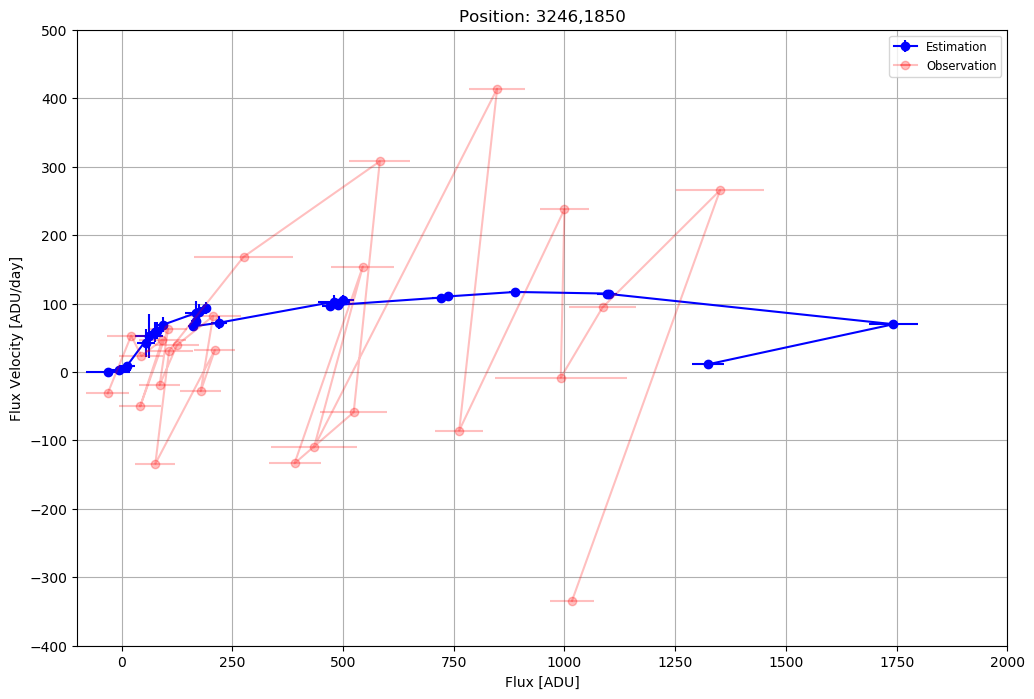
\includegraphics[scale=.5]{images/space_curve.png}
\caption{Espacio de fase de flujo y velocidad de flujo de un candidato. En azul se destaca la estimaci\'on lograda por filtro de Kalman. Notar que en la leyende de la figura, se indica el nivel de complejidad de la curva estimada en t\'erminos de su entrop\'ia \cite{balestrino}, para la curva de flujo y velocidad de flujo estimado.}
\label{fig:sp_st}
\end{figure}
%El estilo de las gr\'aficas de la versi\'on refactorizada respet\'o el dise\~no original de las gr\'aficas, especificados por Pablo Huentelemu.
\chapter{Nueva funcionalidad}
\label{ch:news}
En este cap\'itulo se detallan los cambios realizados a la  manera de ejecutar la pipeline anterior \textsc{RunData} y la modularizaci\'on de las diferentes tareas que involucra este programa, construy\'endose as\'i una nueva clase para la administraci\'on de los procesos: \textsc{RoutineHandler}. Adem\'as se describe la estructura y aspectos esenciales de un nuevo miembro de la familia de filtros de Kalman: \textsf{UnscentedKalman}


\section{Manejo de la rutina: \textsc{RoutineHandler}}

La \textbf{rutina} comprende el proceso de listado de archivos (que en esta nueva versi\'on se realiza con \textsc{DataPicker}), la creaci\'on de una instancia de la familia del filtro de Kalman y la secuencia iterativa de pasos de c\'alculo de flujo, obtenci\'on de estimaciones y el propio proceso de detecci\'on con \textsc{SourceFinder}. Para lograr esto, una instancia de \textsc{RoutineHandler} debe recibir tres archivos descritos a continuaci\'on:
%La \textbf{rutina} se entiende como la ejecuci\'on completa del programa, con la cual se procesan todas las observaciones de acuerdo a una lista de semestres, campos y CCDs . Para esta finalidad se cre\'o una clase llamada \textsc{RoutineHandler} la cual maneja los archivos de entrada de:

\begin{itemize}
\item Lista de campos, CCDs, semestres y, alternativamente, las coordenadas de alg\'un objeto de inter\'es, en un archivo CSV (en este mismo orden) y con el encabezado \texttt{Field, CCD, Semester, POS\_Y, POS\_X}. En caso de no adjuntar las coordenadas en los campos de posici\'on, se puede rellenar con un gui\'on (`-'). En el constructor este archivo se recibe como \texttt{obs\_index\_path}.
\item Diccionario de directorios y expresiones regulares de las ubicaciones de los archivos y sus nombres, respectivamente (archivo de formato CSV). En el constructor de la clase este archivo se denomina como \texttt{route\_templates}.
\item Diccionario de umbrales y par\'ametros relevantes en la ejecuci\'on del programa, as\'i como el tipo de filtro a usar (archivo de formato CSV). En el constructor se denomin\'o \texttt{settings\_file}.
\end{itemize}
\bigskip
Adem\'as de estos archivos se debe especificar el \'indice de la fila a procesar de la lista de campos (\texttt{index}), CCDs y semestre (primer archivo de entrada). Esto se hizo as\'i con la finalidad de facilitar la paralelizaci\'on de los an\'alisis de diferentes conjuntos de datos. Por lo tanto el constructor de \textsc{RoutineHandler} queda como sigue:

\begin{center}
\texttt{RoutineHandler(obs\_index\_path, route\_templates, settings\_file, index)}
\end{center}

Los m\'etodos de esta clase se encuentran en el Ap\'endice \ref{subs:a4}, y ejemplos de los archivos de entrada \texttt{obs\_index\_path}, \texttt{route\_templates} y \texttt{settings\_file} en las secciones \ref{subs:sn_list}, \ref{subs:a1} y \ref{subs:settings_file}, respectivamente.     

\begin{figure}
\centering
\includegraphics[scale=.5]{/home/paloma/Documents/Memoria/Code/sif2/sif2_act}
\caption{Rutina del programa refactorizado.}
\label{fig:new_routine}
\end{figure}  


\section{\textsc{Filtro de Kalman Unscented}}
El dise\~no de la nueva clase de filtro se realiz\'o continuando con la arquitectura del patr\'on Strategy, definiendo los m\'etodos de predicci\'on y correcci\'on en instancias de clases que implementen las interfaces \textsc{IPredict} e \textsc{ICorrect} respectivamente: \textsc{UnscentPredict} y \textsc{UnscentCorrect}.

\subsection{La clase \textsc{UnscentedKalman}}

El filtro Unscented se desarroll\'o en la clase \textsc{UnscentedKalman}, la cual encierra los m\'etodos de predicci\'on y correcci\'on (descritos en el Cap\'itulo \ref{ch:background}, subsecci\'on \ref{ssec:ukf}) implementados en \texttt{predict} y \texttt{correct}.
\bigskip

El constructor de esta clase requiere como argumentos de entrada los siguientes par\'ametros:

\begin{itemize}
\item \texttt{f\_func:} Funci\'on usada para obtener el primer conjunto de puntos sigma para el per\'iodo de predicci\'on. Consiste en una funci\'on vectorial que se aplica sobre cada elemento de una matriz cuya dimensi\'on es la misma que la de la matriz de estado. Corresponde a la funci\'on principal con la que se aplicar\'a el modelo no lineal en el proceso de predicc\'on.
\item \texttt{h\_func:} Funci\'on usada para obtener el segundo conjunto de puntos sigma durante el proceso de correcci\'on. Su aplicaci\'on procede de la misma forma que la descrita para \texttt{f\_func}. Participa en el proceso de correcci\'on.
\item \texttt{f\_args:} Corresponde a una lista de n\'umeros reales de largo dos. El primer valor corresponde a la potencia o grado de la funci\'on mientras que el segundo t\'ermino corresponde al factor que la multiplica. Estos valores est\'an asociados a la funci\'on \texttt{f}.
\item \texttt{h\_args:} Corresponde a una lista de n\'umero reales de largo dos. El primer valor corresponde a la potencia o grado de la funci\'on mientras que el segundo t\'ermino corresponde al factor que la multiplica. Estos valores est\'an asociados a la funci\'on \texttt{h}.
\item \texttt{alpha:} T\'ermino que indica que tan separados se encuentran los puntos sigma en torno a la media (junto a \texttt{kappa}). Por lo general su valor oscila entre $10^{-4}$ y $1$. 
\item \texttt{beta:} Describe el valor de $\beta$ el cual incorpora conocimiento \textit{a priori} sobre la distribuci\'on de las variables de estado. Para distribuciones gaussianas, tiene un valor de $\beta=2$. 
\item \texttt{kappa:} Corresponde a un par\'ametro de escalamiento secundario en la distancia de los puntos sigma a la media. Su valor va entre $0$ y $3-N$ \cite{wan}.
\item \texttt{sigma\_a:} Varianza asociada a la variable de control $\Delta t$. La funci\'on no lineal se aplicar\'a sobre el paso del tiempo.
\item \texttt{image\_size:} Dimensiones de la imagen de flujo. Corresponde a una \textit{tupla}.
\end{itemize}

Al inicializar una instancia de esta clase, se calculan tanto los pesos como el t\'ermino $\lambda$, los cuales dependen de los par\'ametros: $\beta$, $\kappa$ $\alpha$ y N (o cantidad de variables de estado). Ver Ecuaciones \ref{eq:eq20} y \ref{eq:eq21}.
\bigskip

Como parte de la familia de \textsc{KalmanFilter} posee el m\'etodo \texttt{update}, desde el cual se llama a \texttt{predict} y a \texttt{correct}, conservando la firma.
 
\subsection{Predicci\'on}
La predicci\'on de este filtro se implement\'o, como se mencion\'o anteriormente, en la clase \textsc{UnscentedPredict} (que implementa a \textsc{IPredict}). Para instanciar esta clase se debe entregar como argumento al constructor: un puntero a funci\'on (que puede o no ser lineal) \texttt{f\_func} y sus argumentos en \texttt{f\_args}, los pesos asociados a la media \texttt{W\_m} y la covarianza \texttt{W\_c} de predicci\'on, el coeficiente $\lambda$ (\texttt{lambda\_}), la cantidad de variables de estado medidas (en este modelo, se trata de dos: flujo y velocidad de 
flujo, por ende dos) \texttt{N}, la varianza $\sigma_a$ (\texttt{sigma\_a}) y la dimensi\'on de las im\'agenes \texttt{image\_size}. Por lo tanto la firma del constructor queda como sigue:
\bigskip
\begin{center}
\texttt{UnscentedPredict(f\_func, f\_args, Wm, Wc, lambda\_, N, sigma\_a, image\_size)}
\end{center}
\bigskip

Se destaca que tantos los pesos como el valor de $\lambda$ se mantienen constantes durante todo el proceso de predicci\'on y estimaci\'on, valores con los cuales se obtienen los puntos sigma y el valor medio al propagar la funci\'on \texttt{f\_func} (ver Ecuaci\'on \ref{eq:eq18}).
\bigskip

La salida de este m\'etodo est\'a compuesta por la matriz de estado predicha, la predicci\'on de la covarianza y los puntos sigma guardados en la variable \texttt{Xs} de la implementaci\'on.

\subsection{Correcci\'on}
El proceso de correcci\'on est\'a implementado en la clase \textsc{UnscentedCorrect} la cual implementa la interfaz \textsc{ICorrect} redefiniendo el m\'etodo \texttt{correct} para esta versi\'on del filtro. De acuerdo al proceso de correcci\'on para el funcionamiento del filtro se deben definir las funciones $f(\cdot)$ y $h(\cdot)$, adem\'as requiere de los pesos calculados previmente (Ecuaci\'on \ref{eq:eq20}).
\bigskip

El constructor de esta clase posee la siguiente firma.

\bigskip
\begin{center}
\texttt{UnscentedCorrect(f\_func, h\_func, f\_args, h\_args,  Wm, Wc, lambda\_, N, image\_size)}
\end{center}




Durante la correcci\'on se escogen nuevamente $2N+1$ puntos sigma en torno al estado predicho (fase previa) (ver Ecuaci\'on \ref{eq:eq24}), sin embargo los valores de los pesos y de $\lambda$ son los mismos usados durante la fase de predicc\'on, cambiando s\'olo la funci\'on que se propaga sobre este nuevo conjunto de puntos: $h(\dot)$ (expresada como \texttt{h\_func}). 
\bigskip

\subsection{Funciones auxiliares}
Se desarrollaron diferentes funciones auxiliares para apoyar el c\'alculo de las matrices:
\begin{itemize}
\item \texttt{sigma\_points(mean\_, cov\_, lambda\_, N):}\\
Funci\'on con la cual se calculan los puntos sigma a partir de la media de las variables de estado, la covarianza, el valor de $\lambda$ y el n\'umero de variables de estado, N. Utiliza para esta finalidad, la descomposici\'on de Cholesky.
\item \texttt{unscent\_weights(kappa, alpha, beta, N):}\\
M\'etodo con el que se calculan los pesos a partir de los valores de $\kappa$, $\alpha$, $\beta$ y N (n\'umero de variables de estado). 
\item \texttt{perform(func, *args):}\\
Funci\'on auxiliar con la cual se recibe un puntero a otra funci\'on vectorial (destinada a ser aplicada sobre un conjunto de puntos sigma) y un n\'umero arbitrario de argumentos, dependiendo de la necesidad de la misma funci\'on.
\item \texttt{propagate\_func(func, Wm, Wc, Xs, *args, N):}\\
Funci\'on con la que se propaga la funci\'on \texttt{func} sobre el conjunto de puntos sigma \texttt{Xs} usando los pesos de media y covarianza \texttt{Wm} y \texttt{Wc}, respectivamente, adem\'as del n\'umero de variables de estado, N. Adem\'as, recibe el argumento \texttt{args} que corresponde a una tupla de entradas propias de la funci\'on \texttt{func}. 
\end{itemize}

Estas funciones est\'an implementadas en el script \texttt{unscented\_utils}.

\chapter{Resultados}
\label{ch:resultados}
En este cap\'itulo se exponen resultados y an\'alisis de diferentes pruebas realizadas con la nueva versi\'on desarrollada del programa. La primera de las pruebas consiste en medir el desempe\~no de esta pipeline en t\'erminos de tiempo de ejecuci\'on y uso de memoria principal ocupada al procesar tres datasets (usados en el cap\'itulo \ref{ch:prev_work}) asociados a supernovas encontradas por HiTS\cite{hits}: SN14, SN18 y SN80. El segundo conjunto de experimentos corresponde al procesamiento de los 93 conjuntos de datos asociados a las supernovas encontradas por HiTS en el semestre de 2015. En ambos tipos de pruebas se busca comparar el rendimiento y los resultados del programa al emplear los diferentes filtros de Kalman implementados. Finalmente se muestran algunos resultados espec\'ificos obtenidos con el filtro unscented.
\bigskip


Para todas las experiencias se emple\'o umbrales de flujo y velocidad de flujo estimada de 200 [ADU] y 50 [ADU/d\'ia]. Adem\'as todas las im\'agenes procesadas poseen la misma dimensi\'on: $4094 \times 2046$ de alto por ancho, por lo que el campo \texttt{image\_size} de todos los filtros se configuraron en (4094, 2046). Por cada filtro se emplearon los siguientes valores de par\'ametros:

\subsection*{Filtro de Kalman B\'asico}
\begin{itemize}
\item \texttt{sigma\_a}: Se ocup\'o un valor de 0,1. Este valor se ajust\'o despu\'es de realizar diferentes pruebas variando este par\'ametro entre 100 y $10^{-4}$. Este t\'ermino es empleado durante el proceso de predicci\'on y tambi\'en fue usado para ejecutar las pruebas con la versi\'on anterior del programa. 
\item \texttt{init\_var}: La varianza inicial de flujo y velocidad de flujo se estableci\'o con un valor de 100,0. Tal como se emple\'o en el programa original.
\item Se determin\'o 0,0 como valor inicial para las estimaciones de flujo y velocidad de flujo (estado). Fue el mismo valor usado para las pruebas realizadas con el programa original.
\end{itemize}
\subsection*{Filtro de Kalman de m\'axima correntrop\'ia}
\begin{itemize}
\item \texttt{sigma\_a}: Se emple\'o valor 0,1. Este valor es usado, al igual que en el caso del filtro b\'asico, durante el proceso de predicci\'on (mismo m\'etodo).
\item \texttt{sigma}: Se estableci\'o un valor de 1000,0 para la desviaci\'on est\'andar por defecto, en caso de no usar optimizaci\'on de Silverman durante proceso de correcci\'on (valor determinado en la versi\'on original del programa).
\item \texttt{silverman}: \texttt{False}. Para estas pruebas no se us\'o el m\'etodo de Silverman para obtener distribuci\'on ya que la implementaci\'on en el programa original se encuentra incompleta (por lo que una nueva implementaci\'on de esta funci\'on en el software desarrollado en este trabajo queda pendiente para trabajo futuro). 
\item \texttt{std\_factor}: Se estableci\'o como 100,0. Al no usarse el m\'etodo de Silverman, tampoco se hace uso de este valor (valor establecido en la versi\'on original del programa).
\item \texttt{epsilon}: Se asign\'o valor de $10^{-6}$, como error m\'aximo. Es el mismo usado en la versi\'on anterior del programa.
\item \texttt{max\_iter}: Se consider\'o 10 como n\'umero m\'aximo de iteraciones, que es el n\'umero definido por defecto (en el dise\~no del programa original).  
\item \texttt{init\_var} : La varianza inicial de flujo y velocidad de flujo se estableci\'o con un valor de 100.0, tal como se hizo con la versi\'on original.
\item Se determin\'o 0,0 como valor inicial para las estimaciones de flujo y velocidad de flujo. Este valor se us\'o igualmente para las pruebas ejecutadas con el programa original.

\end{itemize}
\subsection*{Filtro de Kalman Unscented}
\begin{itemize}
\item \texttt{f\_func:} Se defini\'o una funci\'on no lineal de grado 1,5 (informaci\'on entregada en \texttt{f\_args}).
\item \texttt{h\_func:} Se estableci\'o como la funci\'on identidad.
\item \texttt{f\_args:} El grado de la funci\'on se defini\'o como 1,5 y un factor de 1,0 (por tanto corresponde a la lista [1,5; 1,0]).
\item \texttt{h\_args:} Para estas pruebas se defini\'o como una lista vac\'ia ya que $h(\cdot)$ se trata de la funci\'on identidad.
\item \texttt{alpha:} Se estableci\'o como 0,001. Ya que con este valor se detectaron algunas supernovas de HiTS. A mayores valores disminuyen el n\'umero de candidatos encontrados (se probaron con valores de 0,0001 a 10).
\item \texttt{beta:} Se le asign\'o un valor de 2,0. Se asumi\'o distribuci\'on normal de las variables de estado\cite{matsinos}. 
\item \texttt{kappa:} Se le asign\'o un valor de 0,0. Se asumi\'o distribuci\'on normal de las variables de estado \cite{matsinos}.
\item \texttt{N:} Al tratarse de dos variables de estado, se establece \texttt{N}=2.
\item \texttt{sigma\_a}: Se defini\'o como 0,1. Se consider\'o usar el mismo valor para este par\'ametro de acuerdo a los resultados obtenidos con los filtros b\'asico y de m\'axima correntrop\'ia, ya que los resultados variaban negativamente (disminuyendo candidatos encontrados) al tomar valores (potencias de diez) mayores o menores a este n\'umero.    
\end{itemize}
Las condiciones iniciales del filtro unscented fueron diferentes a las definidas para los filtros b\'asico y de m\'axima correntrop\'ia, ya que se consider\'o la primera medici\'on de flujo y su varianza para inicializar las matrices de estado y covarianza. Esto debido a que la funci\'on no lineal depende de un $\Delta t$ medido desde cierta \'epoca $t_0$. Para estos experimentos se defini\'o $t_0$ como la primera \'epoca de observaci\'on (los otros m\'etodos dependen de la diferencia temporal entre una \'epoca y otra). Por tanto, se configur\'o el flujo inicial al valor del flujo calculado de la primera \'epoca. Adem\'as, la varianza del estado del flujo fue definida como la matriz de varianza de flujo calculado.


\section{Desempe\~no}
En esta secci\'on se describen los resultados obtenidos durante las experiencias de medici\'on de desempe\~no de la nueva versi\'on del programa en t\'erminos de tiempo y memoria principal usada. 
\bigskip

Las pruebas se realizaron usando el mismo conjunto de datos utilizado para medir el desempe\~no del programa original 
(Cap\'itulo \ref{ch:prev_work}), adem\'as se emplearon como herramientas de medici\'on igualmente el perfilador de memoria \texttt{mem\_profiler} y la librer\'ia \textsc{Resource}\footnote{M\'etodo \texttt{get\_rusage}}. Del mismo modo en que se llevaron a cabo las pruebas usando el programa original, se emple\'o un computador personal de 8 GB de RAM, con un procesador de 2,8 GHz de frecuencia.  

\subsection{Tiempo de ejecuci\'on}
Las Tablas \ref{tab:t7}, \ref{tab:t9} y \ref{tab:t11} muestran los resultados de tiempo medido en segundos de cada una de las partes del proceso de la rutina principal, para los tres datasets usando los filtros b\'asico, de m\'axima correntrop\'ia y unscented, respectivamente. 

\begin{table}[h!]
\centering
\caption{Tiempo de ejecuci\'on en segundos de cada proceso involucrado, usando el filtro de Kalman b\'asico refactorizado: c\'alculo de flujo, estimaci\'on de estados, detecci\'on de candidatos y guardado de candidatos resultantes en caso de haberlos. La \'ultima fila describe el tiempo promedio que toma por observaci\'on (en segundos igualmente) para cada uno de los procesos. }
\begin{tabular}{|l|r|r|r|r|}
\hline
\textbf{ID} & \textbf{C\'alc. Flujos [s]} & \textbf{Estim. KF [s]} &  \textbf{Detecci\'on [s]}  & \textbf{Obt. Candidatos [s]}\\ \hline \hline
SN14        & 297,93            & 28,36        &  33,53 & 0,00 \\ \hline
SN18            & 255,07             & 22,41         & 34,32  & 0,00\\ \hline
SN80            & 199,16             & 17,73         &   25,02 & 0,00 \\ \hline \hline
%Media & 303.08 &  26.23 & 37.83 & 0.01\\\hline 
$\bar{t}/Obs$ & 11,20 &  1,02 & 1,39 & 0,00\\\hline 
\end{tabular}
\label{tab:t7}
\end{table}

\begin{table}[h!]
\centering
\caption{Tiempo de ejecuci\'on en segundos de cada proceso involucrado, usando el filtro de Kalman de m\'axima correntrop\'ia refactorizado: c\'alculo de flujo de las im\'agenes, estimaci\'on de estado, detecci\'on de fuentes y guardado de candidatos. La \'ultima fila describe el tiempo promedio que toma por observaci\'on (en segundos) para cada una de las tareas.}
\begin{tabular}{|l|r|r|r|r|}
\hline
\textbf{ID} & \textbf{C\'alc. Flujos [s]} & \textbf{Estim. KF [s]} &  \textbf{Detecci\'on [s]}  & \textbf{Actual. Candidatos [s]}\\ \hline \hline
SN14        & 289,59            & 491,08        &  34,04 & 0,00 \\ \hline
SN18            & 256,95             & 437,37         &  33,00  & 0,00\\ \hline
SN80            & 199,98             & 346,98         &   24,96 & 0,00 \\ \hline \hline
%Media & 303.08 &  26.23 & 37.83 & 0.01\\\hline 
$\bar{t}/Obs$ & 11,00 &  19,06 & 1,38 & 0,00\\\hline 
\end{tabular}
\label{tab:t9}
\end{table}

\begin{table}[h!]
\centering
\caption{Tiempo de ejecuci\'on en segundos de cada tarea, usando el filtro de Kalman unscented: c\'alculo de flujo, estimaci\'on de filtros, detecci\'on de fuentes y guardado de candidatos. La \'ultima fila describe el tiempo promedio que toma por observaci\'on (en segundos) para cada uno de los procesos.}
\begin{tabular}{|l|r|r|r|r|}
\hline
\textbf{ID} & \textbf{C\'alc. Flujos [s]} & \textbf{Estim. KF [s]} &  \textbf{Detecci\'on [s]}  & \textbf{Actual. Candidatos [s]}\\ \hline \hline
SN14        & 280,67            & 342,88        &  123,68 & 0,01 \\ \hline
SN18            & 243,96             & 293,05         &  122,09  & 0,00\\ \hline
SN80            & 190,43             & 231,34         &   74,48 & 0,00 \\ \hline \hline
%Media & 303.08 &  26.23 & 37.83 & 0.01\\\hline 
$\bar{t}/Obs$ & 10,65 &  12,93 & 4,73 & 0,00\\\hline 
\end{tabular}
\label{tab:t11}
\end{table}
A todos estos resultados se les ha agregado la medici\'on de tiempo promedio por imagen (ya que las secuencias poseen largos diferentes). De estos resultados es posible deducir que el tiempo de c\'alculo de flujo por \'epoca siempre toma alrededor de 11,0 segundos. Esto es claro debido a que el proceso de c\'alculo de flujo es independiente del filtro escogido. Los tiempos de estimaci\'on de estado, por el contrario, var\'ian de filtro en filtro. Tomando mayor tiempo al usar el filtro de m\'axima correntrop\'ia. Sin embargo, opuesto a lo que se esperaba (ya que el proceso de detecci\'on ocurre una vez realizada la estimaci\'on de estado) el filtro unscented presenta un tiempo de detecci\'on casi cuatro veces mayor a los tiempos medidos en los otros filtros; esto se podr\'ia deber a las operaciones lineales realizadas durante el proceso de correcci\'on ya que existir\'ia mayor consumo de RAM. 
\bigskip

Con los filtros b\'asico y de m\'axima correntrop\'ia no se encontraron candidatos en ninguno de los datasets. Esto probablemente puede deberse al cambio en el filtrado de las im\'agenes generado por el proceso de \textit{refactoring}, siendo un proceso m\'as riguroso en la nueva versi\'on, algunas im\'agenes u archivos del dataset de SN14 fueron descartados. No ocurri\'o lo mismo con el filtro unscented al ejecutar la pipeline sobre los datos de la supernova SN14, ya que se encontraron canditatos. Sin embargo, al ser candidatos no confirmados por HiTS, pueden corresponder efectivamente otro tipo de objetos (no necesariamente supernovas), por lo que tendr\'ia que estudiarse su curva de luz o la curva generada por su espacio de estados (es decir, determinar \'indice de entrop\'ia de la curva).
\bigskip

La totalidad y el promedio del tiempo que toma la ejecuci\'on de la pipeline con los tres filtros sobre los datasets se muestran en la Tabla \ref{tab:time}, en donde figuran los resultados de los filtros b\'asico, de correntrop\'ia m\'axima y unscented, respectivamente.
\bigskip

\begin{table}
        
        \caption{Tiempo de exploraci\'on (para detecci\'on de candidatos) para cada uno de los filtros. La \'ultima fila corresponde a tiempo (en segundos) total promedio por observaci\'on. A la izquierda, tiempo empleado usando la nueva versi\'on de filtro de Kalman b\'asico. En el centro, los resultados de tiempo correspondientes al filtro de Kalman de m\'axima correntrop\'ia. A la derecha, resultados correspondientes al filtro unscented.}
            \footnotesize
\begin{tabular}{|l|r|}
\hline
\textbf{ID} & \textbf{Tiempo total [s]} \\ \hline
\hline
SN14  & 359,82 \\\hline
SN18  & 311,8\\\hline
SN80  & 241,91 \\\hline\hline
%Media & 367.15 & 374.83 & 741.98  \\\hline
 $\bar{t}/Obs. $& 13,61 \\\hline 
\end{tabular}
\hfill
\begin{tabular}{|l|r|}
\hline
\textbf{ID} & \textbf{Tiempo total [s]} \\ \hline
\hline
SN14  & 814,71 \\\hline
SN18  & 727,32\\\hline
SN80  & 571,92 \\\hline\hline
%Media & 367.15 & 374.83 & 741.98  \\\hline
 $\bar{t}/Obs. $& 31,58 \\\hline 
\end{tabular}
                \hfill
\begin{tabular}{|l|r|}
\hline
\textbf{ID} & \textbf{Tiempo total [s]} \\ \hline
\hline
SN14  & 747,24 \\\hline
SN18  & 659,1\\\hline
SN80  & 496,25 \\\hline\hline
%Media & 367.15 & 374.83 & 741.98  \\\hline
 $\bar{t}/Obs. $& 28,32 \\\hline 
\end{tabular}
                \label{tab:time}
            \end{table}


De los resultados expuestos sobre el tiempo total de ejecuci\'on se desprende que la pipeline demora menos con el filtro b\'asico, mientras que con el de m\'axima correntrop\'ia es con el toma mayor tiempo.

\subsection{Uso de memoria}
Las Figuras \ref{fig:mem_new_kbf}, \ref{fig:mem_new_mcc} y \ref{fig:mem_ukf} muestran el comportamiento del consumo de memoria (en mebibytes) en el tiempo (en segundos) al usar la nueva versi\'on del filtro b\'asico, de m\'axima correntrop\'ia y el nuevo filtro unscented, respectivamente, ejecutando la pipeline refactorizada sobre los tres conjuntos de datos (SN14, SN18 y SN80). 
\bigskip

\begin{figure}[h!]
\centering
\subfloat[Memoria ocupada en SN14]{\label{fig:new_kbf_14}{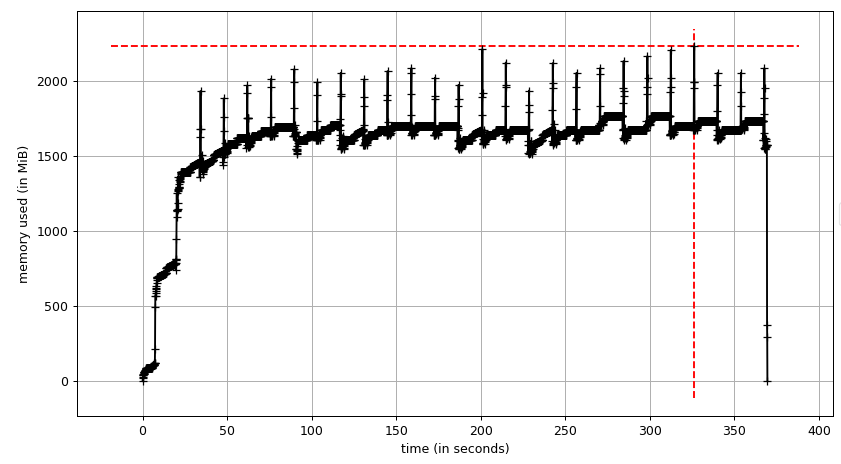
\includegraphics[width=0.5\textwidth]{images/results/sn14_new_bk}}}\hfill
\subfloat[Memoria ocupada en SN18]{\label{fig:new_kbf_18}{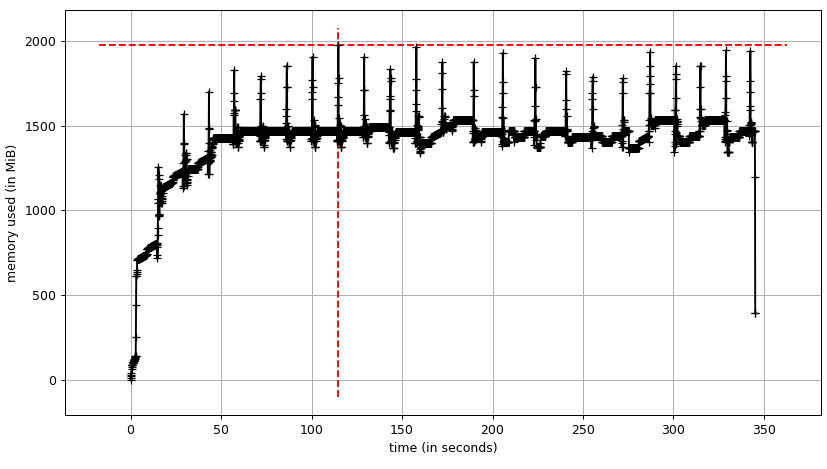
\includegraphics[width=0.5\textwidth]{images/results/sn18_new_bk}}}\vfill
\subfloat[Memoria ocupada en SN80]{\label{fig:new_kbf_80}{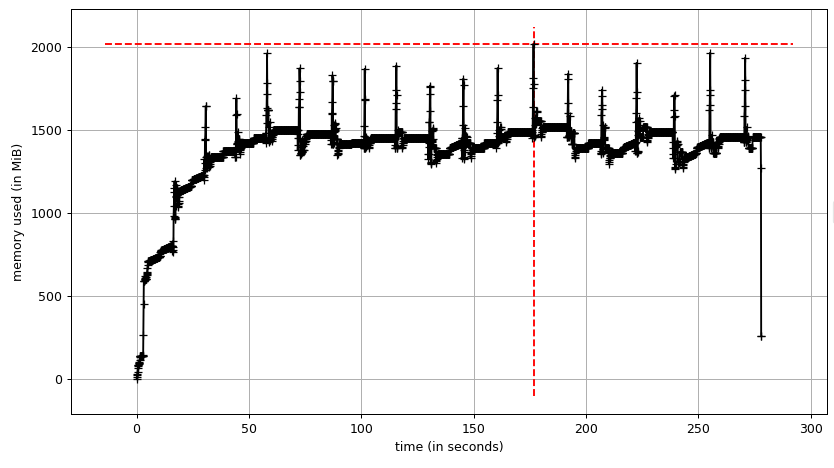
\includegraphics[width=0.5\textwidth]{images/results/sn80_new_bk}}}
\caption{Comportamiento de la memoria (en mebibytes) durante la ejecuci\'on para los tres conjuntos de datos usando el filtro de Kalman B\'asico.}
\label{fig:mem_new_kbf}
\end{figure}

De la Figura \ref{fig:mem_new_kbf} se desprenden los m\'aximos alcanzados durante cada ejecuci\'on (en cada \textit{dataset}) con el filtro b\'asico. Los resultados en megabytes (MB) se listan en la Tabla \ref{tab:mem3}, a la izquierda.
\pagebreak

\begin{table}
        
\caption{Comparaci\'on de la memoria principal (en unidades de MB) usada durante la ejecuci\'on del programa para los tres filtros. A la izquierda, los resultados correspondientes al usar filtro de Kalman B\'asico. En el centro, memoria ocupada usando el filtro de Kalman de m\'axima correntrop\'ia. A la derecha, memoria ocupada usando filtro de Kalman unscented.}
            \footnotesize
\begin{tabular}{|l|r|}
\hline
\textbf{ID} & Memoria [MB]\\\hline\hline
SN14 & 2347,78\\\hline
SN18 & 2254,93\\\hline
SN80 & 2365,07\\\hline
\end{tabular}
                \hfill
\begin{tabular}{|l|r|}

\hline
\textbf{ID} & Memoria [MB]\\\hline\hline
SN14 & 3359,54\\\hline
SN18 & 3350,53\\\hline
SN80 & 3330,93\\\hline
\end{tabular}
                \hfill
\begin{tabular}{|l|r|}

\hline
\textbf{ID} & Memoria [MB]\\\hline\hline
SN14 & 4827,82\\\hline
SN18 & 4835,96\\\hline
SN80 & 4821,89\\\hline
\end{tabular}
                \label{tab:mem3}
            \end{table}



\begin{figure}[h!]
\centering
\subfloat[Memoria ocupada en SN14]{\label{fig:new_mcc_14}{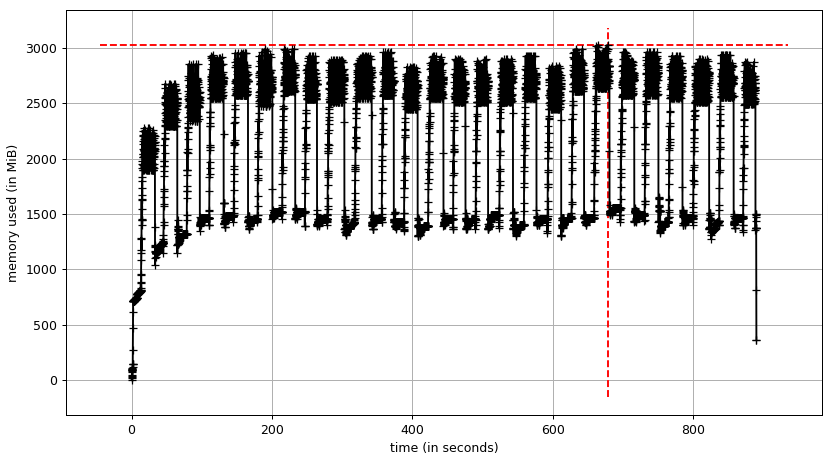
\includegraphics[width=0.5\textwidth]{images/results/sn14_new_mcc}}}\hfill
\subfloat[Memoria ocupada en SN18]{\label{fig:new_mcc_18}{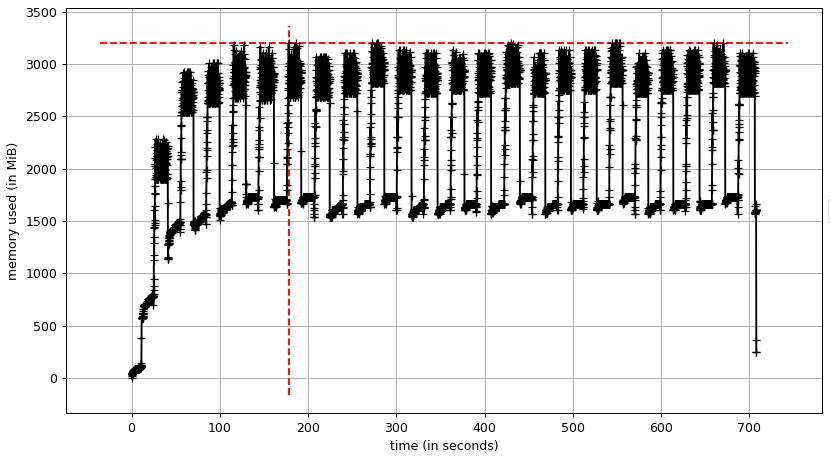
\includegraphics[width=0.5\textwidth]{images/results/sn18_new_mcc}}}\vfill
\subfloat[Memoria ocupada en SN80]{\label{fig:new_mcc_80}{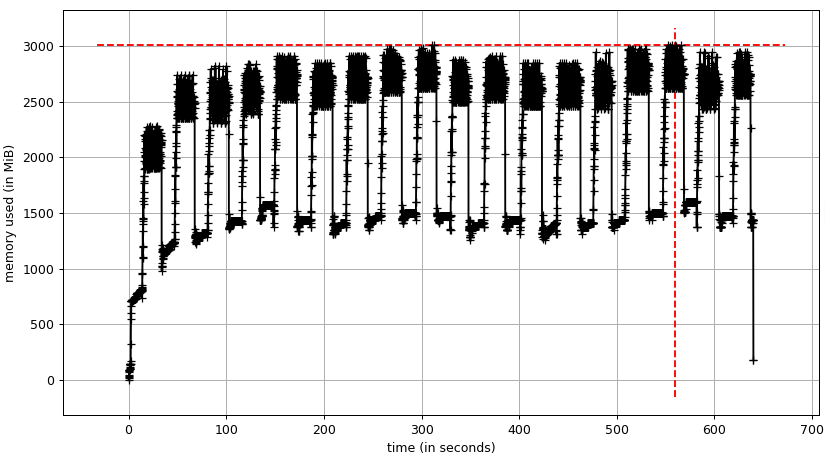
\includegraphics[width=0.5\textwidth]{images/results/sn80_new_mcc}}}
\caption{Comportamiento de la memoria (en mebibytes) durante la ejecuci\'on para los tres conjuntos de datos. En los tres lanzamientos se us\'o el filtro de Kalman de m\'axima correntrop\'ia.}
\label{fig:mem_new_mcc}
\end{figure}

De las series mostradas en la Figura \ref{fig:mem_new_mcc} se obtienen los m\'aximos alcanzados de memoria principal ocupada al utilizar el filtro de m\'axima correntrop\'ia listados en la Tabla \ref{tab:mem3} (centro). 
\bigskip


\begin{figure}[h!]
\centering
\subfloat[Memoria ocupada en SN14]{\label{fig:ukf_sn14}{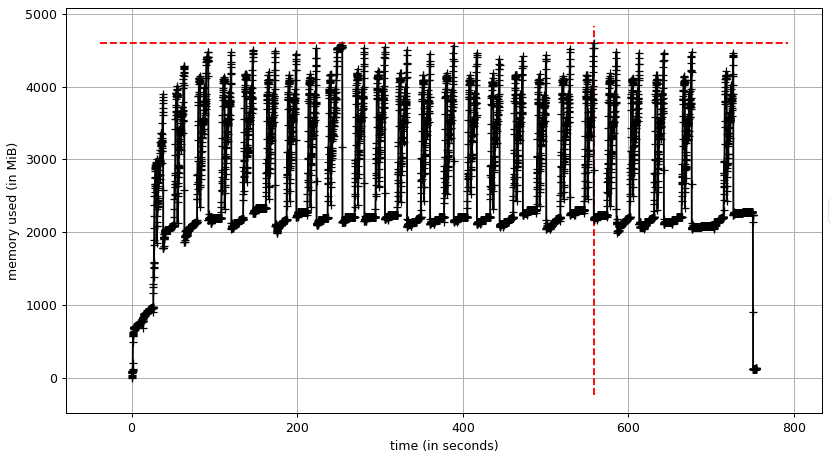
\includegraphics[width=0.5\textwidth]{images/results/sn14_ukf}}}\hfill
\subfloat[Memoria ocupada en SN18]{\label{fig:ukf_sn18}{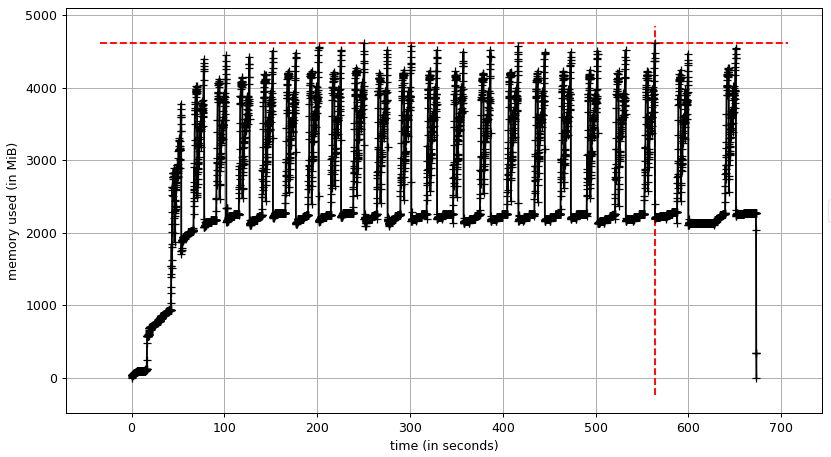
\includegraphics[width=0.5\textwidth]{images/results/sn18_ukf}}}\vfill
\subfloat[Memoria ocupada en SN80]{\label{fig:ukf_sn80}{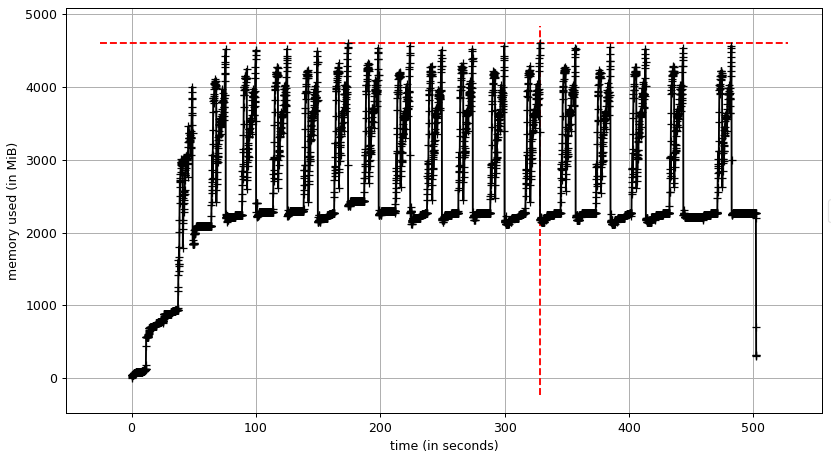
\includegraphics[width=0.5\textwidth]{images/results/sn80_ukf}}}
\caption{Comportamiento de la memoria (en mebibytes) durante la ejecuci\'on para los tres conjuntos de datos. En los tres lanzamientos se us\'o el filtro de Kalman unscented.}
\label{fig:mem_ukf}
\end{figure}



Los resultados de memoria principal muestran un uso intensivo de esta al usar el filtro unscented (ver Tabla \ref{tab:mem3}, derecha). Esto puede ser debido a la serie de operaciones lineales que se debe realizar al momento de predecir y corregir. Tambi\'en se desprende que el uso de memoria es menor con el filtro b\'asico.
\bigskip
 
\section{Detecci\'on}
En esta secci\'on se exponen los resultados obtenidos al procesar los datos de las 93 supernovas con los tres filtros implementados en Leftraru. En particular se muestran las cantidades de verdaderos positivos, falsos negativos, falsos positivos y el n\'umero de conjunto de datos que no pudieron ser procesados por no contar con alg\'un tipo de imagen o archivo necesario para su procesamiento (en este caso, fue la falta de im\'agenes de diferencia). Se considera como falso positivo todo aquello que no est\'e catalogado como supernova de acuerdo a HiTS; es decir, estrellas variables u otro tipo de objetos celestes, rayos c\'osmicos, junto a ruido en la intensidad de los p\'ixeles, etc.
\bigskip

Los par\'ametros usados por cada filtro son los mismos descritos al inicio de este cap\'itulo.

\subsection{Filtros b\'asico y de m\'axima correntrop\'ia}
La Tabla \ref{tab:tpfn_new} muestra los resultados obtenidos con la nueva versi\'on de la pipeline, empleando los filtros refactorizados b\'asico y de m\'axima correntrop\'ia.
\bigskip

\begin{table}[h!]
\centering
\caption{N\'umero de verdaderos positivos (TP), falsos negativos (FN) y falsos positivos (FP) encontrados usando cada uno de los filtros en el conjunto de datos de HiTS. La cuarta columna de valores muestra la cantidad de conjuntos de datos que no pudieron ser procesados.}
\begin{tabular}{|l|r|r|r|r|}
\hline
\textbf{Filtro} & \textbf{TP} & \textbf{FN} & \textbf{FP} & \textbf{NaN}\\ \hline
Básico          & 36          & 54          & 37 &  3 \\ \hline
M\'ax. Corr.             & 36          & 54          & 40  & 3 \\ \hline
\end{tabular}
\label{tab:tpfn_new}
\end{table}
\bigskip

De la Tabla \ref{tab:tpfn_new} se obtiene que el filtro de m\'axima correntrop\'ia encuentra la misma cantida de supernovas conocidas que el filtro b\'asico, y detecta m\'as falsos positivos. Sin embargo cabe recalcar que para esta experiencia no se us\'o el m\'etodo de Silverman para estimar $\sigma$ en el proceso de correcci\'on, por lo que podr\'ia existir opciones de mejora.
\bigskip

De acuerdo a la Tabla \ref{ap:tab1}, Ap\'endice \ref{ap:pip_ref} varias de las detecciones ocurren despu\'es  del per\'iodo de alta cadencia (despu\'es de MJD 57075,00) y pr\'acticamente no hay diferencia entre ambos filtros. Lo primero puede deberse a que es necesario cumplir las condiciones mencionadas en el Ap\'endice \ref{ap:sourcefinder} en los m\'etodos de la clase \textsc{SourceFinder} por cuatro \'epocas consecutivas para emitir una alerta. Por otro lado otras detecciones realizadas por ambos filtros ocurrieron en un per\'iodo bastante alejado del intervalo de alta cadencia, por lo que el distanciamiento entre las observaciones puede haber favorecido a la detecci\'on.
\bigskip
  

\subsection{Filtro unscented}
Con el filtro unscented se realizaron dos pruebas. En ambos casos se asumi\'o la funci\'on $h(\cdot)$ como la funci\'on identidad. En cambio la funci\'on $f(\cdot)$ tom\'o dos formas no lineales en funci\'on de $\Delta t$: $f(\Delta t) = (\Delta t)^{1.5}$ y $f(\Delta t) = (\Delta t)^{2}$. Los resultados obtenidos se muestran en la Tabla \ref{tab:tpfn_ukf}.

\begin{table}[h!]
\centering
\caption{N\'umero de verdaderos positivos (TP), falsos negativos (FN) y falsos positivos (FP) encontrados usando el filtro unscented para dos tipos de funciones no lineales: $f(\Delta t) = (\Delta t)^{1.5}$ y $f(\Delta t) = (\Delta t)^{2}$, sobre el dataset de HiTS. La tercera columna de valores muestra la cantidad de conjuntos de datos que no puedieron ser procesados.}
\begin{tabular}{|l|r|r|r|r|}
\hline
\textbf{Filtro} & \textbf{TP} & \textbf{FN} & \textbf{FP} & \textbf{NaN}\\ \hline
$\Delta t^{1.5}$          & 2          & 87          & 110 &  3 \\ \hline
$\Delta t^{2}$             & 3          & 87          & 108  & 3 \\ \hline
\end{tabular}
\label{tab:tpfn_ukf}
\end{table}
\bigskip

Se observa que bajo la configuraci\'on seleccionada de valores de par\'ametros, el desempe\~no de la detecci\'on es bastante pobre. No obstante se debe considerar la posibilidad de mejorar este resultado estudiando condiciones iniciales, valores de par\'ametros y en particular, las funciones a utilizar ($f(\cdot)$ y $h(\cdot)$).
\bigskip

Para observar si el filtro unscented est\'a trabajando como se espera, es posible visualizar que est\'a sucediendo con las estimaciones y los valores de flujo con alguna de sus detecciones. Se seleccion\'o una de las supernovas encontradas por este filtro en el CCD N2, campo 7 usando una funci\'on $f(\Delta t) = \Delta t^{2}$.

\begin{figure}
\centering
\includegraphics[scale=0.5]{/home/paloma/Documents/Memoria/results/RESULTS/lc_sem_15A_field_07_ccd_N2_obj_0.png}
\caption{En la primera gr\'afica de arriba hacia abajo se muestra el comportamiento del flujo medido y el flujo predicho y estimado. En esta representaci\'on se observa que el flujo se dispara a partir de la fecha 57075. De la misma forma, se dispara las velocidades de flujo estimado y predicho de acuerdo al segundo gr\'afico. El siguiente esquema indica el crecimiento de \textit{flags} de invalidez de los p\'ixeles  mientras que la \'ultima imagen da cuenta del r\'apido crecimiento de las varianzas y covarianzas de estimaci\'on y predicci\'on de las variables de estado. }
\label{ukf_rlc}
\end{figure}

\begin{figure}
\centering
\includegraphics[scale=0.5]{/home/paloma/Documents/Memoria/results/RESULTS/stamps_sem_15A_field_07_ccd_N2_obj_0.png}
\caption{Representaci\'on en p\'ixeles de lo que sucede con el flujo observado, las estimaciones y los \textit{flags} de los p\'ixeles. Se distingue la saturaci\'on sobre las matrices de flujo y velocidad estimada.}
\label{ukf_stamp}
\end{figure}

\begin{figure}
\centering
\includegraphics[scale=0.5]{/home/paloma/Documents/Memoria/results/RESULTS/space_states_sem_15A_field_07_ccd_N2_obj_0.png}
\caption{Se observa el comportamiento conjunto del flujo y velocidad estimados. El r\'apido crecimiento de ambas variables es bastante notable}
\label{ukf_rss}
\end{figure}

De acuerdo a las Figuras \ref{ukf_rlc}, \ref{ukf_stamp} y \ref{ukf_rss} uno de los problemas que adolece este filtro es el de crecimiento r\'apido, por lo que de alguna forma se debe contrarrestar esta gran alza trabajando,  tal vez, sobre la funci\'on de predicci\'on $f(\cdot)$.

\section{Observaciones}
Respecto de las detecciones obtenidas con los filtros b\'asico y de m\'axima correntrop\'ia tanto para esta versi\'on como para la original, se detectaron el mismo  n\'umero de supernovas: treinta y seis. Sin embargo disminuyeron notablemente los falsos positivos respecto de la versi\'on orignal y adem\'as se encontraron tres supernovas m\'as de las confirmadas por HiTS. Esto \'ultimo se piensa puede deberse a un nuevo ordenamiento y filtrado m\'as precisos de los archivos necesarios para ejecutar la rutina.
\bigskip

Por otro lado en t\'erminos de desempe\~no, si bien la nueva versi\'on ha podido disminuir tiempos de ejecuci\'on, a\'un no se logra disminuir la cantidad de memoria principal usada respecto del programa antecesor al emplear los filtros b\'asico y de m\'axima correntrop\'ia.  

%\chapter{An\'alisis}
\section{Desempe\~no}

\chapter{Conclusi\'on}
\label{ch:conclusion}

Se propuso una nueva versi\'on optimizada del software implementado originalmente por Pablo Huentelemu destinado a la detecci\'on de supernovas, obteni\'endose tambi\'en una familia de filtros de Kalman para el an\'alisis de im\'agenes astron\'omicas que puede ser f\'acilmente extendida agregando nuevos m\'etodos de estimaci\'on basados en el filtro de Kalman. Esta extensi\'on es facilitada gracias al patr\'on Strategy empleado en el dise\~no.
\bigskip

Por otro lado, otro de los beneficios adquiridos en esta nueva versi\'on es el control sobre los argumentos de entrada del programa. Anteriormente, las expresiones regulares de los nombres de los archivos ten\'ian que ser escritos expl\'icitamente en el c\'odigo del programa. Sin embargo el c\'odigo redise\~nado en este trabajo permite la recepci\'on de estas expresiones regulares en un archivo de texto plano por lo que el usuario s\'olo debe entregar las rutas y expresiones regulares correspondientes de las im\'agenes y archivos en este documento. Adem\'as, cabe destacar que igualmente se independizaron del c\'odigo los valores de entrada de umbrales y de par\'ametros requeridos en las diferentes rutinas entreg\'andose de la misma forma en un archivo de texto. Es decir se logr\'o evitar el \textit{hard-coding} presente en la versi\'on anterior de la pipeline.
\bigskip

Se debe agregar, que dentro de los cambios agregados a la nueva versi\'on de la pipeline se acort\'o tiempo del proceso ya que a priori se asume que no se conoce ninguna supernova, es decir, el programa no tiene porqu\'e saber si existe un candidato conocido, por lo que los resultados de los potenciales aspirantes a supernova son tratados ecu\'animamente, y por tanto no se discrimina en la informaci\'on obtenida en los resultados al ser guardada en disco. Por ende, el an\'alisis se realiza en una pasada (lo que le permite demorarse la mitad del tiempo original) y no en dos como se realizaba antiguamente.
\bigskip

Respecto de las pruebas realizadas en la evaluaci\'on de las versiones original y nueva, se observa que efectivamente la nueva versi\'on de los filtros b\'asico y de m\'axima correntrop\'ia logran detectar m\'as supernovas que sus respectivas versiones originales (considerando el n\'umero de datasets sobre los cuales se trabaj\'o), adem\'as de reducir el n\'umero de falsos positivos para el mismo conjunto de umbrales. Este resultado se presume que puede ser debido a la mejora en el ordenamiento de los datos de entrada ya que este es aplicado sobre todos los datasets de entrada, tanto a im\'agenes FITS como a archivos de extensi\'on NPY necesarios para la rutina y no s\'olo sobre las primeras como lo realiza el programa original. Del an\'alisis de desempe\~no se desprende que entre las versiones antigua y refactorizada se observa que hay una mejora los tiempos de procesamiento. Sin embargo se mantiene el uso de memoria principal, tanto para el filtro b\'asico como el de m\'axima correntrop\'ia. 
\bigskip

Se refactoriz\'o igualmente el proceso de visualizaci\'on de resultados; con esta nueva versi\'on no s\'olo es posible observar las series de tiempo de la evoluci\'on de las mediciones y observar el comportamiento de los p\'ixeles, flujos y estimaciones gr\'aficamente (como estampillas) sino adem\'as se puede visualizar el resultado de las estimaciones de estado para alg\'un candidato espec\'ifico en el espacio de fase, indicando fecha de detecci\'on (como MJD) y el valor de la complejidad de la curva generada en t\'erminos de su entrop\'ia.
\bigskip

Se implement\'o adem\'as un nuevo miembro de la familia de filtros de Kalman el cu\'al permite realizar aproximaciones con funciones que dependan del paso del tiempo respecto de alg\'un instante de referencia particular. Sin embargo los primeros resultados de este filtro dan cuenta de que se hace necesario estudiar y probar nuevos conjuntos de par\'ametros, condiciones iniciales y funciones, ya que para este trabajo s\'olo se utiliz\'o un rango acotado de estos elementos. Igualmente falt\'o explorar el comportamiento del filtro de m\'axima correntrop\'ia usando el m\'etodo de Silverman.  
\bigskip

Por otra parte se estima que el hecho de que los datos usados para la realizaci\'on de este trabajo presenten un muestreo irregular complica la obtenci\'on de buenos resultados en el proceso de detecci\'on ya que durante la correcci\'on del filtro de Kalman, se requiere una observaci\'on (medici\'on) para realizar las estimaci\'on y por tanto, afecta la siguiente predicci\'on aumentando su incerteza si entre observaciones ha transcurrido demasiado tiempo.
\bigskip 

\section{Trabajo futuro}

Uno de los aspectos pendientes y que se esperar\'ia trabajar en el futuro es el estudiar la variaci\'on de resultados del filtro unscented usando diferentes funciones no lineales. Adem\'as investigar que sucede al variar los par\'ametros como $\sigma_a$. De la misma forma ser\'ia deseable explorar lo que ocurre con el filtro de m\'axima correntrop\'ia al momento de usar el m\'etodo de Silverman.
\bigskip

Por otra parte queda tambi\'en pendiente, el estudiar el comportamiento de los resultados al variar los umbrales relacionados con la estimaci\'on realizada por el filtro de Kalman y que son usados en la fase de reconocimiento de candidatos (en la clase \textsc{SourceFinder}).
\bigskip

Los m\'etodos presentados podr\'ian ser usados en la detecci\'on de estrellas variables aplicando un filtro que distinga tendencias decrecientes en la luminosidad de estos objetos; por lo que una extensi\'on prometedora de este sistema podr\'ia dise\~narse  para reconocer alternancia en los reg\'imenes creciente y decreciente, haciendo uso de la estructura de clases dada por el patr\'on Strategy en el modelo del filtro.
\bigskip



% Apéndices
%\printglossaries
\section*{Glosario}

\begin{itemize}
\item{\textbf{\'Etendue}}\\
\label{a1:etendue}
Es un par\'ametro que caracteriza c\'omo var\'ia la amplitud de la difusi\'on de un haz de luz, de acuerdo con el \'angulo abarcado o en la superficie iluminada. Es el producto de su area transversal (normal a la direcci\'on de propagaci\'on) y del \'angulo s\'olido que la subtiende.


\item{\textbf{PSF}}\\
\label{a1:psf}
Corresponde a la respuesta instrumental a una fuente de luz puntual, cuya radiaci\'on debe atravesar la atm\'osfera terrestre y los lentes del telescopio. La distorsi\'on puede ser interpretada como la convoluci\'on de la imagen por un kernel. \cite{huentelemu}. Ver imagen \ref{fig:a1}

\begin{figure}[h]
\centering
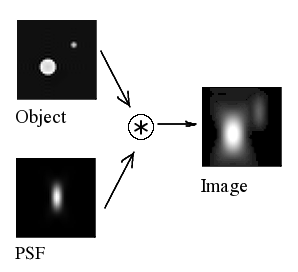
\includegraphics[scale=.5]{images/psf}
\caption{Ejemplo de distorsi\'on de una fuente al aplicar un kernel de PSF espec\'ifico. El resultado se observa en el cuado \textit{Image}.}
\label{fig:a1}
\end{figure}

\item{\textbf{Airmass}}\label{ap:airmass}\\
Es el largo del camino de que le toma a los rayos de una cuerpo celeste atravesar la atm\'osfera. A medida que los rayos van penetrando la atm\'osfera estos se van atenuando por la absorci\'on y el proceso conocido como scattering. 
\end{itemize}
\bigskip
% Bibliografía
\bibliographystyle{abbrv}
\bibliography{./bibliography/tesis}

% Adicionales
%\begin{additional} 
%\section{Capítulo Adicional que no es apéndice}
%\end{additional}

% Apéndices
\begin{appendix} 
\section{Glosario}

\begin{enumerate}
\item{\textbf{Etendue}}\\
\label{a1:etendue}



\item{\textbf{PSF}}\\
\label{a1:psf}
Corresponde a la respuesta instrumental a una fuente de luz puntual, cuya radiaci\'on debe atravesar la atm\'osfera terrestre y los lentes del telescopio. La distorsi\'on puede ser interpretada como la convoluci\'on de la imagen por un kernel. \cite{huentelemu}. Ver imagen \ref{fig:a1}

\begin{figure}[h]
\centering
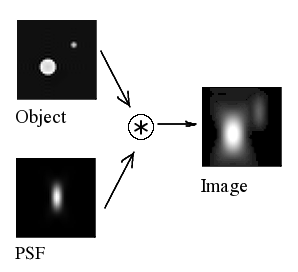
\includegraphics[scale=.5]{images/psf}
\caption{Ejemplo de distorsi\'on de una fuente al aplicar un kernel de PSF espec\'ifico. El resultado se observa en el cuado \textit{Image}.}
\label{fig:a1}
\end{figure}

\item{\textbf{Airmass}}\label{ap:airmass}\\
Es el largo del camino de que le toma a los rayos de una cuerpo celeste atravesar la atm\'osfera. A medida que los rayos van penetrando la atm\'osfera estos se van atenuando por la absorci\'on y el proceso conocido como scattering. 
\end{enumerate}
\bigskip

\section{Refactoring}
\subsection{Librer\'ias usadas para el refactoring}
\label{subs:a0}
Versi\'on de Python: 3.5
\begin{itemize}
\item \textbf{\texttt{pandas}: 0.24.4}
\item \textbf{\texttt{matplotlib}: 2.2.2}
\item \textbf{\texttt{numpy}: 1.13.3}
\item \textbf{\texttt{mahotas}: 1.4.4}
\item \textbf{\texttt{astropy}: 3.0.2}
\end{itemize}
\subsection{Rutas a directorios y expresiones regulares de archivos}
\label{subs:des_rutas}
Los campos se describen a continuaci\'on:
\begin{itemize}
\item \textbf{\texttt{maskDir}}: Directorio donde se almacenan las im\'agenes m\'ascara (im\'agenes que identifican p\'ixeles que no deben ser considerados).
\item \textbf{\texttt{scienceDir}}: Directorio donde se almacenan las im\'agenes cient\'ificas (im\'agenes base ya preprocesadas).
\item \textbf{\texttt{diffDir}}: Directorio donde se almacenan las im\'agenes de diferencia (resta entre las im\'agenes base y cient\'ifica).
\item \textbf{\texttt{psfDir}}: Directorio donde se encuentran los modelos de psf (ap\'endice \ref{a1:psf}) usados para la determinaci\'on del flujo.
\item \textbf{\texttt{invDir}}: Directorio que guarda las im\'agenes correspondientes a la varianza inversa (\textit{peso} de cada pixel en t\'erminos de ruido: a menor peso, mayor ruido).
\item \textbf{\texttt{afluxDir}}: Directorio que contiene los archivos de extensi\'on \texttt{NPY} dentro de los cuales se guarda el valor de la variable \texttt{aflux}.
\item \textbf{\texttt{maskRegEx}}: Expresi\'on regular con la que es posible identificar el nombre de las im\'agenes m\'ascara en disco siguiendo el path \texttt{maskDir}.
\item \textbf{\texttt{scienceRegEx}}: Expresi\'on regular con la que es posible identificar el nombre de las im\'agenes cient\'ificas en disco siguiendo el path \texttt{scienceDir}.
\item \textbf{\texttt{diffRegEx}}: Expresi\'on regular con la que se identifican el nombre de las im\'agenes de diferencia en disco siguiendo el path \texttt{diffDir}.
\item \textbf{\texttt{invRegEx}}: Expresi\'on regular con la que es posible identificar el nombre de las im\'agenes de la varianza inversa siguiendo el path \texttt{invDir}.
\item \textbf{\texttt{afluxRegEx}}: Expresi\'on regular con la que se identifica el nombre de los archivos \textit{match} que contienen el valor de \texttt{aflux}. Estos archivos est\'an ubicados en el path \texttt{afluxDir}.
\item \textbf{\texttt{psfRegEx}}: Expresi\'on regular que describe el nombre de las im\'agenes que guardan el modelo de PSF en el directorio \texttt{psfDir}.
\end{itemize}

\subsection{Archivo de entrada: configuraci\'on de paths}
\label{subs:a1}
\VerbatimInput{/home/paloma/Documents/Memoria/Code/sif2/inputs/dirset_leftraru.txt}


%\section{Nueva funcionalidad}
%\subsection{Modelo de archivo de almacenamiento de resultados}
\subsection{M\'etodos}
\subsubsection{Lectura y preparaci\'on de im\'agenes}
\label{subs:a2}
A continuaci\'on se enumeran los diferentes m\'etodos que intervienen en la recolecci\'on de los datos a ser le\'idos:

\begin{itemize}
\item \textbf{\texttt{config\_reg\_expressions(semester, field, ccd)}}\\
Este m\'etodo recibe como par\'ametros strings que indiquen el semestre (\texttt{semester}), el campo (\texttt{field}) y el ccd (\texttt{ccd}) que se quiere analizar. Puede hacerse uso de los valores de las variables de instancia que la misma clase \textsc{DataPicker} recibe en su constructor. Con estos strings se establecen las rutas de los directorios de las im\'agenes y las expresiones regulares de los nombres de las mismas.
\bigskip

\item \textbf{\texttt{collect\_data()}}\\
Esta funci\'on se encarga de recolectar la ruta completa de las diferentes im\'agenes (m\'ascaras, im\'agenes cient\'ificas, de diferencia, etc.). Para esta finalidad se hace uso del m\'etodo \texttt{walking\_through\_files}. 
\bigskip

\item \textbf{\texttt{walking\_through\_files(regex, dir)}}\\
M\'etodo con el cual se recorren las rutas definidas en los pasos anteriores y se agrupan los nombres completos (directorio incluido) de las im\'agenes ubicadas en el directorio \texttt{dir} y posean un nombre de patr\'on que siga la expresi\'on regular \texttt{regex}.
\bigskip

\item \textbf{\texttt{filter\_science\_images()}}\\
Filtra im\'agenes cient\'ificas de acuerdo a su airmass (Ap\'endice  \ref{ap:airmass}), seleccionando aquellas obtenidas en fechas cuyo valor de airmass calculado es menor a 1,7. De esta secuencia de im\'agenes cient\'ificas resultante se obtiene una lista de fechas que cumplen esta condici\'on, medidas en t\'erminos de \textit{d\'ia juliano modificado} o \textit{Modified Julian Date} (MJD) de tipo punto flotante. Estos valores son ordenados de forma creciente.%las fechas en que las observaciones fueron hechas en t\'erminos de \textit{d\'ia juliano modificado} o \textit{Modified Julian Date} (MJD) como variables de punto flotante.
\bigskip

\item \textbf{\texttt{select\_fits(dir)}}\\
Selecciona y ordena los elementos de la lista de im\'agenes de formato \textsc{fits} del directorio \texttt{dir} usando la lista de MJDs (guardada en la variable de instancia \texttt{mjd} de la clase) generada en \texttt{filter\_science\_images()} escogiendo s\'olo aquellas cuyas fechas correspondan a las fechas indicadas.  %cronol\'ogico (i.e. de acuerdo a la secuencia de MJD encontrada en \texttt{filter\_science\_images()}).
\bigskip

\item \textbf{\texttt{select\_npys(dir, ref\_dir, init\_index, n\_pos, rest\_len)}}:\\
Debido a que los archivos de extensi\'on NPY no poseen la variable MJD en su estructura (en los archivos \textsc{fits} encontramos este valor en el header de la imagen) deben de filtrarse de forma diferente. Para este caso el filtrado de este tipo de archivos se lleva a cabo a trav\'es de la revisi\'on de sus nombres, ya que comparten patrones con los nombres de ciertas im\'agenes \textsc{fits}. Por ejemplo, los nombres de las im\'agenes de PSF, de formato NPY, poseen similitud con los nombres de las im\'agenes \textsc{fits} de diferencia; igualmente los archivos \texttt{aflux} de formato NPY poseen parecidos en sus nombres con las im\'agenes cient\'ificas. Esta similitud es medida a trav\'es de un substring diferente para cada tipo de archivo NPY, definido por la posici\'on inicial \texttt{init\_index}, en el nombre del archivo \textsc{fits} y largo \texttt{rest\_len}. \texttt{n\_pos} indica la posici\'on de un car\'acter espec\'ifico `` \_ '' en dicho substring para validar esta comparaci\'on.

\end{itemize}


\subsection{Diccionario de par\'ametros y umbrales}
\label{subs:a3}
El diccionario de umbrales y par\'ametros de configuraci\'on contiene la siguiente lista de valores:

\begin{itemize}
\item \texttt{imgHeight}: Altura de las im\'agenes cient\'ificas en p\'ixeles. Esta dimensi\'on se propaga al resto de im\'agenes y matrices. Las im\'agenes usadas en este trabajo poseen una altura de 4094 p\'ixeles. 
\item \texttt{imgWidth}: Ancho de las im\'agenes cient\'ificas en p\'ixeles. Esta dimensi\'on se propaga al resto de im\'agenes y matrices, y en este trabajo las respectivas im\'agenes poseen un ancho de 2046.
\item \texttt{filter}: Tipo de filtro (\texttt{basic}, \texttt{mcc} o \texttt{ukf}).
\item \texttt{results}: Directorio de resultados (donde se guardan las coordenadas de los candidatos encontrados junto a lista de \'epocas en que fueron detectados) en formato NPZ.
\item \texttt{init\_var}: Varianza inicial que tendr\'an las matrices de covarianza durante el proceso de estimaci\'on con los filtros de Kalman. 
\item \texttt{flux\_thresh}: Umbral para estado de flujo obtenido con Kalman. Es un valor determinado por el usuario (en este trabajo se defini\'o como 200). 
\item \texttt{flux\_rate\_thresh}: Umbral para la velocidad de flujo obtenido con Kalman. Es un valor establecido por el usuario (en este trabajo se defini\'o como 50).
\item \texttt{rate\_satu}: Tasa de saturaci\'on.
\item \texttt{sigma\_a}: Varianza de la distribuci\'on de la componente de control ($u_k$) asumiendo normalidad. Es importante al emplear los filtros b\'asico y unscented, ya que corresponde a la desviaci\'on est\'andar de la distribuci\'on normal de la aceleraci\'on originada por cambios no esperados en el modelo (lo que se puede interpretar como ``fuerzas externas'') \cite{ian}.
\item \texttt{epsilon}: Radio de error con que la estimaci\'on por filtro de Kalman de m\'axima correntrop\'ia disminuye la ganancia de Kalman. Corresponde a un criterio de detenci\'on y toma valores entre 0 y 1 (t\'ipicamente, $10^{-6}$)\cite{badong}.
\item \texttt{max\_iter}: N\'umero de iteraciones m\'aximo para el proceso de correcci\'on al usar Kalman de m\'axima correntrop\'ia. 
\item \texttt{silverman}: \textit{Entero}. Toma valor 1 en caso de considerarse, y 0 si no. Se establece si se usa o no la aproximaci\'on de Silverman para determinar ancho de banda del kernel al emplear el filtro de m\'axima correntrop\'ia.
\item \texttt{std\_factor}: Factor de incremento de sigma al usar el m\'etodo de Silverman.
\item \texttt{sigma}: Sigma usado por defecto sin Silverman en la determinaci\'on del kernel durante el proceso de correcci\'on con el Filtro de Kalman de correntrop\'ia m\'axima .
\item \texttt{beta}: Par\'ametro relacionado con la distribuci\'on del estado estimado ($x_k$). Toma valor de $\beta = 2$ para distribuciones normales.
\item \texttt{kappa}: Participa en la regulaci\'on del rango de los valores de los puntos sigma y usualmente toma valores entre 1 y 3N-1 (N corresponde al n\'umero de dimensiones)\cite{wan}. Aporta incremento adicional (ver Ecuaci\'on \ref{eq:eq21}).
\item \texttt{alpha}: Participa en la regulaci\'on del rango de los valores de los puntos sigma, y generalmente toma valores positivos menores o iguales a 1: $10^{-4} \leq \alpha \leq 1 $\cite{wan}. Incrementa el rango en un factor $\alpha$ (ver Ecuaci\'on \ref{eq:eq21}).
\item \texttt{dim}: Cantidad de componentes de estado a medir (en este programa se miden dos: flujo y su velocidad).
\end{itemize}
\subsection{Archivo de entrada: par\'ametro y umbrales}
\label{subs:settings_file}
\VerbatimInput{/home/paloma/Documents/Memoria/Code/sif2/inputs/settings_example.txt}
\subsection{Archivo de entrada: lista de campos, CCDs y semestres (incluye algunas coordenadas)}
\label{subs:sn_list}
\VerbatimInput{/home/paloma/Documents/Memoria/Code/sif2/inputs/hits15.csv}

\subsection{M\'etodos de la clase \textsc{RoutineHandler}}
\label{subs:a4}
\begin{itemize}
\item \texttt{process\_settings():}\\
En este m\'etodo se lee el archivo de diccionario de umbrales y par\'ametros con los que se configurar\'a la toma de decisiones del programa.
\bigskip

\item \texttt{retrieve\_kalman\_filter(kalman\_string):}\\
Corresponde a un m\'etodo auxiliar que es invocado desde \texttt{process\_settings} con el que se crea una instancia del filtro de Kalman a partir de la lectura del archivo de valores, de acuerdo al valor definido por el usuario. Los tres strings v\'alidos para la construcci\'on de una instancia son: `basic', `mcc' y `ukf'. Si se entrega otro tipo de string, se levanta un error.
\bigskip
  
\item \texttt{iterate\_over\_sequences(check\_found\_objects):}\\
Recorre la lista de campos, CCDs y semestres entregada al programa con la consiguiente llamada a \texttt{routine}. Recibe como par\'ametro el argumento \texttt{check\_found\_objects} con el cual se indica si se quiere analizar resultados obtenidos anteriormente (candidatos encontrados), y que es entregado al m\'etodo \texttt{routine} descrito a continuaci\'on.
\bigskip

\item \texttt{routine(semester, field, ccd, results\_path, check\_found\_objects, last\_mjd):}\\
Comprende la rutina principal del programa, es decir, el an\'alisis de las observaciones de un semestre, campo y CCD espec\'ifico. El argumento \texttt{check\_found\_objects} es un boolean e indicar\'a el modo de ejecuci\'on del m\'etodo: si es falso, s\'olo guardar\'a las coordenadas de los candidatos encontrados (si no encontr\'o nada, entonces se guarda una lista vac\'ia) adem\'as de las \'epocas en que fueron detectados. Esta informaci\'on se guarda en un arreglo de diccionarios. Si \texttt{check\_found\_objects} es verdadero, entonces cargar\'a resultados anteriores del directorio de resultados (configurado en \texttt{process\_settings}) para estudiar la presencia de los candidatos encontrados en caso de existir.
\end{itemize}  
\bigskip
%\section{Unit-tests}
%\subsection{Refactoring}
\pagebreak

\section{Detecci\'on usando pipeline original}
\begin{table}[h!]
\small
\centering
\caption{Resultados de \'epocas de detecci\'on en t\'erminos de MJD de las 93 supernovas del conjunto de 2015 de HiTS, usando los filtros implementados originalmente (b\'asico y de correntrop\'ia m\'axima).}
\begin{tabular}{|l|r|r|}
\hline
\textbf{\'Ind.} & \textbf{B\'asico} & \textbf{MCC}   \\
\hline
1&57072,19 & 57072,19 \\
2&-             & -             \\
3&57075,15 & 57075,15 \\
4&57075,21 & 57075,21 \\
5&57072,24 & 57072,24 \\
6&-             & -             \\
7&-             & -             \\
8&57075,10 & 57075,10 \\
9&57075,22 & 57075,22 \\
10&57077,11 & 57077,11 \\
11&57075,20 & 57075,20 \\
12&57072,21 & 57072,21 \\
13&57077,15 & 57077,15 \\
14&-             & -             \\
15&57077,11 & 57077,11\\
16&57077,09 & 57077,09\\
17&57077,11 & 57077,11 \\
18&57090,23 & 57090,23 \\
19&-             & -             \\
20&57077,12   & 57077,12  \\
21&-             & -             \\
22&57077,12 & 57077,12 \\
23&-             & -             \\
24&57077,08  & 57077,08   \\
25&57075,25 & 57075,25 \\
26&-             & -             \\
27&57077,17 & 57077,17 \\
28&-             & -             \\
29&-             & -             \\
30&57072,35 & 57072,35 \\
31&-             & -             \\
32&57075,21 & 57075,21 \\
33&-             & -             \\
34&-             & -             \\
35&-             & -             \\
36&57080,11 & 57080,11 \\
37&57075,21 & 57075,21 \\
38&-             & -             \\
39&-             & -             \\
40&-             & -             \\
41&-             & -             \\
42&-             & -             \\
43&57090,22 & 57090,22\\
44&-             & -             \\
45&-             & -             \\
46&-             & -             \\
47&57075,20 & 57075,20 \\\hline
\end{tabular}
\quad
\begin{tabular}{|l|r|r|}
\hline
\textbf{\'Ind.} & \textbf{B\'asico} & \textbf{MCC} \\
\hline
48&57080,17 & 57080,17 \\
49&57090,24 & 57090,24 \\
50&57075,21 & 57075,21 \\
51&-             & -             \\
52&-             & -             \\
53&-             & -             \\
54&-             & -             \\
55&-             & -             \\
56&57075,11  & 57075,11  \\
57&57095,20 & 57095,20 \\
58&-             & -             \\
59&57095,20 & 57095,20\\
60&-             & -             \\
61&-             & -             \\
62&57095,16 & 57095,16\\
63&-             & -             \\
64&-             & -             \\
65&-             & -             \\
66&-             & -             \\
67&-             & -             \\
68&-             & -             \\
69&-             & -             \\
70&-             & -             \\
71&-             & -             \\
72&-             & -             \\
73&-             & -             \\
74&-             & -             \\
75&-             & -             \\
76&-             & -             \\
77&-             & -             \\
78&-             & -             \\
79&-             & -             \\
80&-             & -             \\
81&-             & -             \\
82&-             & -             \\
83&-             & -             \\
84&-             & -             \\
85&-             & -             \\
86&57080,20 & 57080,20 \\
87&-             & -             \\
88&-             & -             \\
89&-             & -             \\
90&-             & -             \\
91&NaN           & NaN           \\
92&NaN           & NaN           \\
93&NaN           & NaN          \\\hline
\end{tabular}
\label{ap:tab1}
\end{table}
\pagebreak


\section{Detecci\'on usando pipeline refactorizada}
\label{ap:pip_ref}
\begin{table}[h!]
\small
\centering
\caption{Resultados de \'epocas de detecci\'on en t\'erminos de MJD de las 93 supernovas del conjunto de 2015 de HiTS, usando los filtros refactorizados (b\'asico y de correntrop\'ia m\'axima).}
\begin{tabular}{|l|r|r|}
\hline
\textbf{\'Ind.} & \textbf{B\'asico} & \textbf{MCC} \\\hline
1& 57072,19   & 57072,19   \\
2& -              & -              \\
3& 57075,15    & 57075,15     \\
4& -   & -   \\
5& 57072,24   & 57072,24   \\
6& 57077,09   & 57077,09   \\
7& -              & -              \\
8& 57075,10   & 57075,10   \\
9& 57075,22   & 57075,22   \\
10& 57077,11   & 57077,11   \\
11& 57075,20    & 57075,20    \\
12& 57072,14   & 57072,14   \\
13& 57077,15   & 57077,15   \\
14& -    & -    \\
15& 57077,11   & 57077,11   \\
16& 57077,09   & 57077,09   \\
17& 57077,11   & 57077,11   \\
18& -   & -   \\
19& -              & -              \\
20& 57077,18   & 57077,18   \\
21& 57077,12   & 57077,18   \\
22& 57077,12  & 57077,12   \\
23& -              & -              \\
24& 57077,08    & 57077,08             \\
25& 57077,09   & 57077,09   \\
26& -   & -   \\
27& 57077,17   & 57077,17   \\
28& -              & -              \\
29& -              & -              \\
30& 57072,21   & 57072,21   \\
31& -              & -              \\
32& 57075,21   & 57075,21   \\
33& -              & -              \\
34& -              & -              \\
35& 57078,20   & 57078,20   \\
36& 57080,11   & 57080,11   \\
37& -              & -              \\
38& - & - \\
39& -              & -              \\
40& -              & -              \\
41& 57075,08     & 57075,08              \\
42& -              & -              \\
43& 57090,22   & 57090,22   \\
44& -              & -              \\
45& -              & -              \\
46& -              & -              \\
47& 57075,20   & 57075,20   \\\hline
\end{tabular}
\quad
\begin{tabular}{|l|r|r|}
\hline
\textbf{\'Ind.} & \textbf{B\'asico} & \textbf{MCC}\\\hline
48& 57080,11   & 57080,11   \\
49& 57090,24   & 57090,24   \\
50& 57077,18   & 57077,18   \\
51& 57077,13   & 57077,13  \\
52& -              & -              \\
53& -              & -              \\
54& 57095,17              & 57095,17              \\
55& -              & -              \\
56& 57075,11   & 57075,11   \\
57& 57095,20   & 57095,20   \\
58& -              & -              \\
59& -              & -              \\
60& 57095,20              & 57095,20             \\
61& -              & -              \\
62& -   & -   \\
63& -              & -              \\
64& -              & -              \\
65& -              & -              \\
66& 57095,15   & 57095,15   \\
67& -              & -              \\
68& -              & -              \\
69& -              & -              \\
70& -              & -              \\
71& -              & -              \\
72& -              & -              \\
73& -              & -              \\
74& -              & -              \\
75& -              & -              \\
76& -              & -              \\
77& -              & -              \\
78& -              & -              \\
79& -              & -              \\
80& -              & -              \\
81& -              & -              \\
82& -              & -              \\
83& -              & -              \\
84& -              & -              \\
85& -              & -              \\
86& 57090,26   & 57090,26   \\
87& -              & -              \\
88& -              & -              \\
89& -              & -              \\
90& -              & -              \\
91& NaN            & NaN            \\
92& NaN            & NaN            \\
93& NaN            & NaN           \\\hline
\end{tabular}
\label{ap:tab2}
\end{table}
\pagebreak

\section{Detecci\'on usando filtro unscented}
\begin{table}[h!]
\small
\centering
\caption{Resultados de \'epocas de detecci\'on en t\'erminos de MJD de las 93 supernovas del conjunto de 2015 de HiTS, usando el filtro unscented para una funci\'on $f(\Delta t) = \Delta t^{1.5}$ y $f(\Delta t) = \Delta t^{2}$.}

\begin{tabular}{|l|r|r|}
\hline
\textbf{\'Ind.} & \textbf{n=1.5}  & \textbf{n=2.0}  \\\hline
1     & -        & 57072,26 \\
2     & -        & -        \\
3     & -        & -        \\
4     & -        & -        \\
5     & 57072,24 & -        \\
6     & -        & -        \\
7     & -        & -        \\
8     & -        & 57077,09 \\
9     & -        & -        \\
10    & -        & -        \\
11    & -        & -        \\
12    & -        & -        \\
13    & -        & -        \\
14    & -        & -        \\
15    & -        & -        \\
16    & -        & -        \\
17    & -        & -        \\
18    & -        & -        \\
19    & -        & -        \\
20    & 57090,24 & 57090,24 \\
21    & -        & -        \\
22    & -        & -        \\
23    & -        & -        \\
24    & -        & -        \\
25    & -        & -        \\
26    & -        & -        \\
27    & -        & -        \\
28    & -        & -        \\
29    & -        & -        \\
30    & -        & -        \\
31    & -        & -        \\
32    & -        & -        \\
33    & -        & -        \\
34    & -        & -        \\
35    & -        & -        \\
36    & -        & -        \\
37    & -        & -        \\
38    & -        & -        \\
39    & -        & -        \\
40    & -        & -        \\
41    & -        & -        \\
42    & -        & -        \\
43    & -        & -        \\
44    & -        & -        \\
45    & -        & -        \\
46    & -        & -        \\
47    & -        & -        \\\hline
\end{tabular}
\quad
\begin{tabular}{|l|r|r|}
\hline
\textbf{\'Ind.} & \textbf{n=1.5} & \textbf{n=2.0}\\\hline
48    & -        & -        \\
49    & -        & -        \\
50    & -        & -        \\
51    & -        & -        \\
52    & -        & -        \\
53    & -        & -        \\
54    & -        & -        \\
55    & -        & -        \\
56    & -        & -        \\
57    & -        & -        \\
58    & -        & -        \\
59    & -        & -        \\
60    & -        & -        \\
61    & -        & -        \\
62    & -        & -        \\
63    & -        & -        \\
64    & -        & -        \\
65    & -        & -        \\
66    & -        & -        \\
67    & -        & -        \\
68    & -        & -        \\
69    & -        & -        \\
70    & -        & -        \\
71    & -        & -        \\
72    & -        & -        \\
73    & -        & -        \\
74    & -        & -        \\
75    & -        & -        \\
76    & -        & -        \\
77    & -        & -        \\
78    & -        & -        \\
79    & -        & -        \\
80    & -        & -        \\
81    & -        & -        \\
82    & -        & -        \\
83    & -        & -        \\
84    & -        & -        \\
85    & -        & -        \\
86    & -        & -        \\
87    & -        & -        \\
88    & -        & -        \\
89    & -        & -        \\
90    & -        & -        \\
91    & NaN        & NaN        \\
92    & NaN        & NaN     \\
93    & NaN        & NaN      \\\hline
\end{tabular}
\label{ap:tab3}
\end{table}

\end{appendix}



\end{document}